%% Journal version for "Machine Learning" (Springer).
%% Class: sn-jnl.cls, Springer Nature LaTeX template version 3.1 (December 2024),
%% downloaded 2026-11-10 from resource-cms.springernature.com (see NOTES.md).
%% Reference style: sn-apa (author--year, APA list), matching the journal's
%% guidelines (citations by name and year; APA-style reference examples).
\documentclass[pdflatex,sn-apa]{sn-jnl}

\usepackage{graphicx}
\usepackage{multirow}
\usepackage{amsmath,amssymb,amsfonts}
\usepackage{amsthm}
\usepackage{mathtools}
\usepackage[title]{appendix}
\usepackage{xcolor}
\usepackage{textcomp}
\usepackage{manyfoot}
\usepackage{booktabs}
\usepackage{array}
\usepackage{adjustbox}
\usepackage{tikz}
\usepackage{pgfplots}
\pgfplotsset{compat=1.16}
\usepgfplotslibrary{fillbetween}
% Shared TikZ styles for the schematic figures (colours = slots 1-4 of the validated reference palette).
\usetikzlibrary{arrows.meta,positioning,calc,fit,backgrounds,matrix,decorations.pathreplacing}
\definecolor{cBlue}{HTML}{2A78D6}
\definecolor{cOrange}{HTML}{EB6834}
\definecolor{cAqua}{HTML}{1BAF7A}
\definecolor{cViolet}{HTML}{6250D6}
\definecolor{cInk}{HTML}{1D1D1B}
\definecolor{cInkTwo}{HTML}{52514E}
\definecolor{cBand}{HTML}{F0EFEA}
\tikzset{
  nd/.style={circle,draw=cInkTwo,fill=white,line width=0.5pt,inner sep=0pt,minimum size=0.43cm,font=\scriptsize,text=cInk},
  ndh/.style={nd,fill=cBlue!24,draw=cBlue,line width=0.8pt},
  ndr/.style={nd,fill=cOrange!30,draw=cOrange,line width=0.9pt},
  ndl/.style={nd,fill=black!7,draw=black!35,text=black!50},
  ndu/.style={nd,fill=black!6},
  ndsm/.style={nd,minimum size=0.33cm,font=\tiny},
  ar/.style={-{Stealth[length=3pt,width=2.4pt]},draw=cInkTwo!80,line width=0.55pt},
  ars/.style={-{Stealth[length=3.2pt,width=2.6pt]},draw=cOrange,line width=1.2pt},
  arl/.style={-{Stealth[length=3pt,width=2.4pt]},draw=black!30,line width=0.55pt},
  arb/.style={-{Stealth[length=3pt,width=2.4pt]},draw=cBlue,line width=0.9pt},
  un/.style={draw=cInkTwo!80,line width=0.55pt},
  lab/.style={font=\scriptsize,text=cInkTwo},
  labb/.style={font=\scriptsize\bfseries,text=cInk},
  band/.style={fill=cBand,draw=none,rounded corners=2pt},
  box/.style={draw=cInkTwo,rounded corners=2pt,line width=0.6pt,fill=white,align=center,font=\scriptsize,inner sep=3pt},
}

\newcommand{\tikzfig}[1]{\adjustbox{max width=\textwidth,center}{\input{figs/tikz/#1}}}
\usepackage{url}
\usepackage[capitalize,noabbrev]{cleveref}

\theoremstyle{thmstyleone}
\newtheorem{theorem}{Theorem}
\newtheorem{proposition}[theorem]{Proposition}
\newtheorem{lemma}[theorem]{Lemma}
\newtheorem{corollary}[theorem]{Corollary}
\newtheorem{conjecture}[theorem]{Conjecture}
\theoremstyle{thmstylethree}
\newtheorem{definition}[theorem]{Definition}
\theoremstyle{thmstyletwo}
\newtheorem{remark}[theorem]{Remark}

\raggedbottom
\emergencystretch=2em

% ---------- project macros ----------
% Lean names: typeset in tt, breakable at underscores.
\makeatletter
\g@addto@macro{\UrlBreaks}{\do\_}
\makeatother
\newcommand{\lname}[1]{\nolinkurl{#1}}
\newcommand{\lean}[1]{\par\noindent{\footnotesize\textsf{Lean:}~#1}\par}
\newcommand{\nolean}[1]{\par\noindent{\footnotesize\textsf{Lean:}~not machine-checked (#1).}\par}
% Placeholders for results that do not exist yet. Never replace with invented numbers.
\definecolor{phcolor}{RGB}{176,32,32}
\newcommand{\PH}[1]{{\color{phcolor}\textbf{[PLACEHOLDER: #1]}}}

\newcommand{\Es}{E_{\mathrm S}}
\newcommand{\Ex}{E_{\times}}
\newcommand{\Eo}{E_{\circ}}
\newcommand{\Eu}{E_{\uparrow}}
\newcommand{\GT}{G_T}
\newcommand{\GS}{G_{\mathrm S}}
\newcommand{\rel}{\mathrm{rel}}
\newcommand{\anc}{\mathrm{anc}}
\newcommand{\desc}{\mathrm{desc}}
\newcommand{\Src}{\mathrm{Src}}
\newcommand{\srho}{s_\rho}
\newcommand{\neff}{n_{\mathrm{eff}}}
\newcommand{\nhalf}{n_{1/2}}
\newcommand{\atanh}{\operatorname{atanh}}

\begin{document}

\title{Rel-Sortability of Time-Unrolled Causal Graphs}

\author*[1]{\fnm{Quang-Vinh} \sur{Dang}}\email{vinh.dq4@buv.edu.vn}
\affil*[1]{\orgname{British University Vietnam}, \orgaddress{\city{Hung Yen}, \country{Vietnam}}}

\abstract{Hiding the time labels of an unrolled process does not hide the time
order. In a time-unrolled DAG built from a summary graph with self-loops, the
relatives of a variable leave a graph-determined
footprint of time. We follow this footprint through four
questions. First, we compute the rel-sortability of every edge exactly, for
every summary graph and horizon, with its limit and a burn-in (the largest
finite distance in the summary graph) after which the value no longer depends
on the start; the graph statements are machine-checked in Lean~4. The
burn-in is minimal for directed chains (proved for relatives, computed for
values) and can be too long for other graphs. Second, a fixed start inflates the footprint: strongly connected
summary graphs are not protected at short horizons, and the fixed start raised
the order accuracy of a relatives-sorting baseline by 0.13.
Third, we state when relatives can be estimated from one autocorrelated
record. Fourth, controlled tests show that the gain follows the
correlations a test can detect, not the population relatives pattern, and that
the share of the exact gap that is realised grows with sample size (0.18 at
$n=200$, 0.76 at $n=25{,}000$). Tuned DAGMA, NOTEARS and GOLEM-NV
overtook FLOP on in-trees under the fixed start and lost after a burn-in;
variance is involved but does not explain it alone. Real-data support is mostly
negative. Results are for lag-one dynamics; no deployed
generator was found to use the construction as shipped. We propose no new
algorithm.}

\keywords{causal discovery, sortability, time series, benchmark simulation,
formal verification, finite-sample theory}

\maketitle

%=============================================================================
\section{Introduction}
\label{sec:intro}

Simulated benchmarks drive much of causal discovery, and several of their
regularities can be exploited without any causal reasoning. Marginal variances
tend to grow along the causal order (\emph{var-sortability};
\citealp{reisach2021beware}), so a method that sorts by variance does well on
data from common generators, and it explains the strong benchmark performance of some
continuous-optimisation methods, a family that includes NOTEARS
\citep{zheng2018notears}. The
coefficient of determination $R^2$ has the same property and is scale
invariant \citep{reisach2023scale}; internally standardised structural
models are not var-sortable by construction and, empirically, mostly not
$R^2$-sortable \citep{ormaniec2025standardizing}; and \citet{herman2025unitless} relate the
$R^2$ pattern to colliders and confounders and propose a generator that avoids
it. Most recently, \citet{reisach2026topological} defined
\emph{rel-sortability}, which orders a node by the number of its
\emph{relatives} (nodes joined to it by an open path, marginally dependent on
it under faithfulness). Relatives are a property of the graph alone, so the
criterion cannot be removed by reweighting. For random DAGs it is high; for
\emph{time-unrolled} DAGs built from a summary graph with self-loops,
\citet[Thm.~4]{reisach2026topological} show that it tends to $1/2$ if every
weakly connected component of the summary graph is strongly connected, and
they propose such graphs as benchmarks. Only sufficiency is shown in the arXiv
version; they do not analyse the value beyond this case. The preprint fixes neither a horizon nor an initial law for the unrolled
construction, and its data code is not public.

\textbf{The thesis.} Removing the time labels from an unrolled process does not
remove the time order. The order leaves a footprint in label-free data: which
variables are relatives of which, a property of the unrolled graph alone.
\emph{Time order survives label removal as a graph-determined footprint; the
footprint is exactly computable, depends on how a simulation starts, is only
partly visible at realistic sample sizes, and measurably changes what
label-free learners appear to do.} The paper follows this one object through
four questions, and they give it its order.
\textbf{Q1:} what is the footprint exactly, and what does it identify when the
labels are hidden? \textbf{Q2:} how does the start of a simulation shape it?
\textbf{Q3:} how much of it can an estimator see in one finite, autocorrelated
record? \textbf{Q4:} what does it do to label-free learners and to real data?
The questions matter for real time series, whose summary graphs are often
feed-forward (rivers, supply chains, signalling cascades), and for anyone who
builds a benchmark from an unrolled graph.

\begin{figure}[t]
\centering
\tikzfig{fig_hero}
\caption{The idea in one picture. (a) A summary graph with a self-loop at every node.
(b) Its time-unrolled DAG $G_T$ for $T=4$: one column per slice, one row per variable.
The \emph{relatives} of a node are the nodes that share an ancestor with it; the blue nodes
are the eight relatives of $c_2$. (c) A label-free learner receives only the columns of the data, in unknown order.
Counting the partners of each column (here, exactly, the number of relatives $\rho$) still carries the time
order: along every edge of (b) the count either grows or stays equal (for example $c_1\to c_2$: $4\to 8$).
The rest of the paper asks how exactly this footprint can be computed, how a simulation's start changes it,
and how much of it a learner sees.}
\label{fig:hero}
\end{figure}

\textbf{Contributions.} \emph{(Q1) The footprint.} The exact rel-sortability of
every edge of the time-unrolled DAG $\GT$, for every summary graph with
self-loops and every $T$ (\cref{thm:edge}); its limit
$\tfrac12+|\Ex|/(2|\Es|)$ with the rate $\min(\Delta,T{-}1)/(T{-}1)$
(\cref{thm:limit}); and the necessity of the condition of
\citet[Thm.~4]{reisach2026topological} (\cref{cor:iff}). These statements are
machine-checked in Lean~4 (\cref{sec:lean}). When the labels are hidden, the
slice of every column is a graph invariant of the unrolled DAG, its Markov
equivalence class is explicit, and under a fixed start and faithfulness the
unrolled DAG is identified from second moments up to the reversal of isolated
units, with three exact non-identifiability results and one open conjecture
(\cref{sec:ident}). These are paper proofs, conditional on faithfulness, and
no human has read them yet.
\emph{(Q2) The start.} The excess for chains and out-trees is a boundary
effect of the deterministic start (\cref{prop:boundary}). After a latent
burn-in of $B\ge\Delta$ slices, the value is fixed by the \emph{source}
strongly connected components for every $T$ (\cref{thm:stat,cor:statiff}).
This burn-in is sufficient. It is exactly minimal for the one-edge graph
(Lean) and, by an exact argument on paper and exact enumeration, for directed
chains at every length computed (\cref{prop:chainsharp}); it is not minimal in
general: in an enumeration of 726 random summary graphs, $B=\Delta-1$ was
insufficient in 445 and sufficed in 281, and in a second exact computation on
396 random graphs the minimal burn-in was $\Delta$ in 51\% of the cases and up
to four slices shorter in the rest. We have no closed form for the minimal
burn-in of a given graph (\cref{rem:sharp}). Strongly connected
summary graphs are not protected at short horizons: a ring has $\srho(\GT)=1$
for all $T\le p$.
\emph{(Q3) Visibility.} An effective sample size for the relatives test, the
saturation of relatives counts by a latent driver, and the effect of block
means and subsamples (\cref{sec:finsamp}). The proofs are on paper, the
non-asymptotic bounds are loose, and a fixed truncation lag controls the size
only away from a unit root.
\emph{(Q4) Learners and real data} (\cref{sec:experiments}). With the time
labels hidden, the fixed start raised the order accuracy of a relatives-sorting
baseline by $0.13$ in simulations, and the gain replicated under nonlinear
dynamics. All 42 simulated conditions have a positive exact gap and a positive
gain, so agreement in sign does not test the theory. A designed test
(\cref{sec:controls}) separates two readings. Data with the population
relatives of a burn-in but the detectable correlations of the fixed start kept
$0.96$ of the gain, and the share of the exact gap that is realised grew with
the sample size ($0.18$ at $n=200$, $0.76$ at $n=25{,}000$) and with the
spectral radius. The exact gap is therefore the large-sample ceiling, and the
effect realised at a finite sample size is its detectable image. On raw data,
tuned DAGMA, NOTEARS and GOLEM-NV overtook FLOP on in-trees under the fixed
start and lost to it after a burn-in, which our plan had predicted would not
happen. Matching the marginal variances across the two starts removed the
advantage, which points to variance, but imposing the fixed-start variances on
burn-in data restored less than half of it, so the cause is not fully explained
and our theory does not cover it. The real-data studies ask a different
question (can relatives be estimated from one record?) and mostly failed or did
not discriminate; the positive results come from one device, and at the level
of independent runs or stations they cannot reach conventional significance.

\textbf{Scope and status.} The results are for lag-one unrollings with a
self-loop at every node, and the simulations use $n=1000$. The unrolled
construction is a proposal of \citet{reisach2026topological}; our survey of
common generators found none that hands slices to a method that ignores time
order as shipped (\cref{sec:b1}). We propose no new causal-discovery method.
The graph results of Q1 are short consequences of a walk-length lemma and of
\citet[Lemma~1]{reisach2026topological}; their value is that they settle the
value for every summary graph, horizon and start. The finite-sample results use
textbook tools. \Cref{tab:status} lists the status of each claim.

\begin{table}[t]
\caption{Status of the claims of this paper. ``Lean'' means a theorem proved
in Lean~4 (the map from Lean statements to paper statements has not been
checked by a human); ``paper proof'' means a proof in the appendix that no
human has read line by line; ``enumerated'' means exact computation on many
instances, not a proof.}
\label{tab:status}
\centering\small
\setlength{\tabcolsep}{3pt}
\begin{tabular}{>{\raggedright\arraybackslash}p{0.37\textwidth}>{\raggedright\arraybackslash}p{0.27\textwidth}>{\raggedright\arraybackslash}p{0.28\textwidth}}
\toprule
claim & evidence & status \\
\midrule
exact per-edge value, limit, necessity of the condition (Q1) & proof; Lean; 46{,}724 enumerated cases & proved; Lean-checked \\
stationary value after burn-in $B\ge\Delta$ (Q2) & proof; Lean & proved; Lean-checked \\
sharpness of $B\ge\Delta$ (Q2) & Lean for one edge; paper proof for the relatives of chains; exact enumeration for chains ($p\le8$), rings and 396 random graphs; 445 of 726 random graphs fail at $\Delta-1$ & Lean for $\Delta=1$; proved on paper for chain relatives; enumerated for chain $\srho$; not sharp in general \\
limits for random summary graphs (Q2) & paper proof; numerics & paper proof, unread by a probabilist \\
slices, equivalence class, non-identifiability (Q1) & paper proofs; small-case checks & paper proofs, conditional on faithfulness \\
effective sample size, saturation, conditioning (Q3) & paper proofs; simulations; algebra in Lean & paper proofs, asymptotic; bounds loose \\
fixed start raises rel-sortability (Q2, Q4) & simulation, 420 graphs, replicated & supported, positive in all 42 conditions \\
exact gap and the size of the gain (Q4) & post hoc detectability calculation; designed counterfactual and dose tests (\cref{sec:controls}) & the realised effect follows detectable correlation; the exact gap is the large-$n$ ceiling (0.76 of it at $n=25{,}000$) \\
DAGMA and NOTEARS overtake FLOP under a fixed start (Q4) & learner extension, 96 graphs; tuned, variance-matched control, 288 graph-seeds & observed and survives tuning; variance channel by the plan's rule but not sufficient; mechanism not explained; plan predicted otherwise \\
relatives count orients edges in real data (Q3, Q4) & CausalRivers; two Causal Chambers devices (P7--P9, E1, E2, B3) & mostly failed or non-discriminating \\
\bottomrule
\end{tabular}
\end{table}

\textbf{Organisation.} \Cref{sec:related} places the work among studies of
benchmark regularities, time-series causal discovery and identification.
\Cref{sec:theory} answers Q1 and gives the theory part of Q2: the exact values,
the effect of a burn-in, the Lean verification and the identifiability
statements for hidden labels. \Cref{sec:finsamp} answers Q3 and treats block
means and subsamples. \Cref{sec:experiments} answers the empirical part of Q2
and Q4 with the benchmark experiments, the controlled tests of the mechanism and the real-data studies, and
\cref{sec:disc} gives recommendations, limitations and the statement on the use
of AI tools.

%=============================================================================
\section{Related Work and Background}
\label{sec:related}

The question of this section is where the four questions of
\cref{sec:intro} stand in the literature. The paper touches three bodies of
work: studies of what simulated benchmarks reward, time-series causal discovery
together with the generators that supply its test data, and the identification
and finite-sample theory that the later sections use. We discuss each in turn
and then state what is new here and what is not.

\subsection{Sortability and the evaluation of continuous-optimisation learners}
\label{sec:rw-sort}

Continuous-optimisation learners cast structure learning as numerical
optimisation over weighted adjacency matrices. NOTEARS \citep{zheng2018notears}
replaces the combinatorial acyclicity constraint by a smooth function of the
matrix, and later methods change the constraint or the objective: DAGMA
\citep{bello2022dagma} uses a log-determinant characterisation of acyclicity,
and GOLEM \citep{ng2020golem} maximises a likelihood with soft penalties.
Constraint-based search \citep{spirtes2000causation} and greedy score-based
search \citep{chickering2002optimal} remain the classical alternatives, and
FLOP \citep{wienobst2026flop}, a recent discrete-search method, is the
strongest method without time labels in our experiments
(\cref{sec:b1}). All of these are developed and compared mostly on simulated
linear or additive-noise models with random graphs. A regularity of the
generator that tracks the causal order can therefore change a ranking without
any causal reasoning on the part of the learner, and a line of work has
identified such regularities one by one.

\citet{reisach2021beware} showed that in common generators the marginal
variance tends to grow along the causal order (var-sortability). A baseline that
sorts by variance and then regresses is competitive on such data, and
continuous-optimisation methods lose accuracy once the data are standardised.
\citet{kaiser2022unsuitability} reach a related conclusion from the side of the
method: NOTEARS is not scale invariant, it aims at a parsimonious DAG that
explains the residual variance, and the authors conclude that it is unsuited to
identifying causal relationships from data with dimensional quantities.
\citet{reisach2023scale} introduced $R^2$-sortability, the same kind of
regularity measured with a scale-invariant quantity, and a corresponding
sorting baseline. \citet{ormaniec2025standardizing} study internally
standardised structural causal models, which are not var-sortable by
construction and, empirically, mostly not $R^2$-sortable.
\citet{herman2025unitless} relate the $R^2$ pattern to colliders and
confounders and propose a unit-free generator that avoids it and whose
time-series extension starts from the exact stationary distribution.
\citet{reisach2026topological} then defined rel-sortability, which counts the
relatives of a node, that is, the nodes joined to it by an open path. Relatives
depend on the graph alone, so reweighting cannot remove the criterion. For
time-unrolled DAGs built from a summary graph with self-loops they proved that
the criterion tends to $1/2$ when every weak component of the summary graph is
strongly connected, and they proposed such graphs for benchmarks. Their
statement is a sufficient condition. This paper completes it: the exact value of
every edge for every summary graph and horizon, the exact limit, the effect of a
burn-in, and the question of whether the value matters for what learners
recover.

For time series, \citet{lohse2025sortability} adapt var- and $R^2$-sortability
to summary graphs, observe that cyclic pairs push the signal towards $1/2$,
and measure both on river-flow and Causal Chambers data. They give no theorem
and do not study relatives or the way a record is observed. Robustness of
score-matching learners to violated model assumptions has been studied by
\citet{montagna2023assumption}, which is a different mechanism from the
generator regularities above but leads to the same practical caution about
reading benchmark rankings.

Several studies question how far simulated benchmarks resemble the data that
methods meet in practice. \citet{gentzel2019case} argue for evaluating causal
models with interventional measures and empirical data, and
\citet{brouillard2025landscape} review the data sets used in causal discovery
and how they relate to real applications. On the side of simulation design,
\citet{andrews2026daggeneration} propose a DAG adaptation of the onion method,
and \citet{nagarajan2025topology} show for Bayesian structure learning that the
topology of the network changes benchmark outcomes; \citet{vowels2022dya}
survey the structure-learning methods that these comparisons concern. Our
subject is narrower. We take one proposed generator, the time-unrolled
construction, and ask what its start does to the quantities that sorting
baselines exploit.

Our SPADE paper \citep{dang2026spade} introduces a B-spline additive-noise DAG
learner and compares it with DAGMA, GraN-DAG, GOLEM, NOTEARS, SCORE, NoGAM,
PCMCI and VAR-LiNGAM on simulated nonlinear DAGs, with mixed results against
NoGAM. It also reports a graph learned from a financial panel in levels that
collapsed on stationary returns, a reminder that a learned graph can reflect
shared non-stationarity as well as mechanism, which is the situation that the
fixed start creates in simulation.

\subsection{Time-series causal discovery and its generators}
\label{sec:rw-ts}

Methods that use time order go back to Granger causality
\citep{granger1969investigating}. VAR-LiNGAM \citep{hyvarinen2010varlingam}
fits a structural vector autoregression and uses non-Gaussianity to orient the
instantaneous effects. PCMCI and PCMCI+ \citep{runge2019detecting,
runge2020pcmciplus} combine lagged conditional-independence tests with a
momentary-conditional-independence step, the latter also handling contemporaneous
links, and are available in the tigramite package \citep{tigramite}.
DYNOTEARS \citep{pamfil2020dynotears} carries the NOTEARS formulation over to
structural VAR models, and neural Granger methods \citep{tank2021neural} replace
the linear lag effect by a network. All of them are given the time index. Only
a static learner applied to a time-unrolled DAG, as in
\citet{reisach2026topological}, sees the slices as unlabelled variables, and
that is the setting of this paper. Our learner extension in \cref{sec:b1}
therefore compares label-free static methods with PCMCI+ as a labelled
reference.

Benchmarks for the time-indexed methods include the CauseMe platform
\citep{runge2019inferring}, the Causality 4 Climate competition
\citep{weichwald2020causal} and CausalTime \citep{cheng2024causaltime}, which
builds its data from fitted models of real series. A data-generating process
for time-series causal discovery with explicit lag structure is described by
\citet{lawrence2021dgp}. Real records with partial ground truth are rarer; we use
CausalRivers \citep{stein2025causalrivers} and the Causal Chambers
\citep{gamella2025chambers} in \cref{sec:real}. \citet{assaad2022survey}
survey and evaluate time-series discovery methods. Reading a dynamical system
as an unrolled causal graph has its own foundations: \citet{mooij2013ode}
relate ordinary differential equations to structural causal models in the
deterministic case.

How a simulation starts a vector autoregression is old practice in
econometrics. Textbook treatments discuss the initial condition and the choice
between conditioning on it and drawing it from the stationary distribution
\citep{hamilton1994time,lutkepohl2005new,kilian2017structural}, and the effect
of the initial condition on inference for persistent processes has a literature
of its own \citep{muller2003tests}. The fixed start of the unrolled construction
is the case of a zero initial state. What this paper adds is a statement about
the dependence structure: a burn-in of $\Delta$ slices equalises the relatives
of the nodes, whereas making the covariance stationary needs a burn-in that
matches the spectral radius (\cref{sec:b1}). We did not find a treatment of
this distinction for causal-discovery benchmarks.

How these generators start a trajectory matters for the artefact studied here.
We read the source code of the simulators in common use (\cref{app:b1x}). Some
return the series from a fixed start with no burn-in; some discard between a few
steps and several hundred, or a fraction of the series length; and the
unit-free generator of \citet{herman2025unitless} draws the initial lags from
the stationary distribution. Whether the start affects a result also depends on
what is done with the data. A single record passed to a time-series method is
outside the threat model, whereas the time-unrolled construction of
\citet{reisach2026topological} gives every slice, including those right after
the start, to a method that ignores time order. \Cref{sec:b1} states the two
conditions and applies them to each generator.

A related issue is the observation scheme. Block means and subsamples of a
faster process change the model that the analyst sees
\citep{weiss1984systematic,breitung2002temporal} and its identifiability
\citep{gong2015subsampled,hyttinen2016subsampled,gong2017aggregated}. We ask what
they do to the three sortability criteria in \cref{sec:agg}.

\subsection{Tied unrolled models, time labels and identification}
\label{sec:rw-ident}

A time-unrolled DAG with a single transition applied at every step is a dynamic
Bayesian network: a start network and a transition network that is repeated
\citep{friedman1998learning}. When the time labels are known, learning such a
model is standard, because the slices and the tying are given. Hiding the labels
turns the slice structure into something that has to be identified, which is the
question of \cref{sec:ident}. The tied parameters also bear on whether the
usual genericity argument for faithfulness applies. Coloured Gaussian DAG
models, which tie vertex variances or edge weights across colour classes, are
the closest static analogue. \citet{boege2025colored} show that a generic
covariance matrix of an edge-coloured DAG is faithful to the graph, and the
same holds for vertex-coloured DAGs (their Propositions~5.3 and~5.4). They give
an example with vertex and edge colours together that has no faithful
distribution (Example~5.7) and leave open which coloured DAGs admit a faithful
distribution (Question~5.8). Their common-head condition defines the subfamily
on which they prove structural identifiability and run their search algorithm,
and is not part of the faithfulness results. On our reading, the unrolled model
ties the transition weights across slices (an edge colouring) and, when every
slice has the same noise variances, the noise variances (a vertex colouring),
so it is the mixed case for which faithfulness is open. We have not shown that
this reading is right or that the model falls in a class covered by their
positive results.

Two classical facts about time direction enter the non-identifiability results
of \cref{sec:ident}. Time reversal can leave the covariance of a stationary
linear process unchanged \citep{weiss1975time}, and the direction of a time
series can be recovered under non-Gaussian or additive-noise assumptions that we
do not make \citep{peters2009detecting}.

\Cref{sec:labels} asks whether the changing covariance during the transient
after a fixed start carries information about the mechanism. The closest
precedents are identification through heteroskedasticity
\citep{rigobon2003identification,lanne2008identifying,lewis2021identifying},
which needs the covariance of the structural shocks to change across regimes or
over time, and identification of linear stochastic differential equations from
temporal marginals \citep{wang2023generator,guan2026identifying}. Our remark is
a short consequence of the Markov property and is stated to separate the
artefact for label-free methods from information available to methods with
labels.

\subsection{Finite-sample behaviour of dependence tests under autocorrelation}
\label{sec:rw-finite}

Estimating relatives from one record means running marginal independence tests
between series. The distortion of a test for the correlation of two series that
uses the nominal sample size, when the series are autocorrelated, is classical
\citep{bartlett1935,clifford1989,roy1989}. In causal discovery it is usually
handled by effective sample sizes \citep{runge2019detecting,afyouni2019effective}
or by residual-based tests; testing independence of two series through lagged
cross-correlations goes back to \citet{haugh1976checking}. The marginal tests we
analyse are Fisher-$z$ tests of the kind used by the PC algorithm
\citep{spirtes2000causation}. For the variance of the sample correlation we use
the Bartlett form, and for tail and limit statements we rely on standard tools
for quadratic forms of Gaussian processes and for Toeplitz-type functionals
\citep{hsu2012tail,laurent2000adaptive,arcones1994limit,nourdin2011quantitative,
ginovyan2021survey}. Residual confounding by an unreliably measured covariate,
which limits what a partial-correlation test can remove, is documented in
\citet{westfall2016confounding}. Our contribution in \cref{sec:finite} is to
combine these ingredients for the specific statistic that defines relatives, to
make explicit when the plug-in estimate of the effective sample size is
consistent, and to state where a fixed truncation lag breaks the size guarantee.

\subsection{Formal verification}
\label{sec:rw-lean}

The graph results are checked in Lean~4 \citep{demoura2021lean4} with Mathlib
\citep{mathlib2020}. A formally grounded
agentic framework for automated research in causal inference has been described
\citep{tan2026causalsmith}. We are not aware of a Lean formalisation of
rel-sortability or of the unrolled-graph results here, and our development
covers only the deterministic graph and algebra parts (\cref{sec:lean}). No human has yet checked that the Lean statements match the
statements in the paper.

\subsection{Positioning}
\label{sec:rw-pos}

New here are four things, in the order of the questions of \cref{sec:intro}.
First, the exact per-edge value of rel-sortability of a time-unrolled DAG for
every summary graph with self-loops and every horizon, its limit, and a
sufficient burn-in condition, with the graph statements machine-checked; the
burn-in is shown to be needed only for the one-edge graph. Second, a
measurement of what the fixed start does to benchmark results, with
time-stamped plans, replications and every failed prediction reported. Third,
finite-sample statements about estimating relatives from one autocorrelated
record, with their limits. Fourth, identifiability statements for hidden time
labels, conditional on faithfulness. We do not propose a new causal-discovery
method, and the finite-sample and identifiability statements rest on standard
tools and on paper proofs that no human has read line by line.

\textbf{Takeaway.} The nearest work is the sortability line, which supplies
the object (relatives) and the proposed benchmark; econometric practice and
time-series generators supply the notion of a start; the tied-model and
heteroskedasticity literatures frame what labels add. None of them gives the
exact values or measures the effect of the start on label-free learners.

%=============================================================================
\section{Time-Unrolled DAGs: Exact Values, Burn-in and Identifiability}
\label{sec:theory}

\textbf{Question.} What is the footprint of time in the relatives structure of
an unrolled DAG, how does the start of the simulation shape it, and what does
it identify when the labels are hidden? This section collects the
graph-theoretic answers. \Cref{sec:setting} fixes notation, \cref{sec:exact}
gives exact values, limits and the effect of a burn-in,
\cref{sec:labels,sec:ident} ask what the start law and the time labels add, and
\cref{sec:lean} states what is machine-checked.

\subsection{Setting and notation}
\label{sec:setting}

For a directed graph, $\anc(y)$ and $\desc(y)$ contain $y$; the relatives of
$y$ are $\rel(y)=\desc(\anc(y))=\{z:\anc(y)\cap\anc(z)\neq\emptyset\}$ and
$\rho(y)=|\rel(y)|$. For an edge $(x,y)$, $\srho(x,y)=1,\tfrac12,0$ if
$\rho(x)<,=,>\rho(y)$, and $\srho(G)$ is the mean over \emph{edges}, as in
\citet[Eq.~(4)]{reisach2026topological} (quoted verbatim in \cref{app:exact}).
A value $1/2$ means the criterion carries no orientation information.

A \emph{summary graph} $\GS=(V,\Es)$ has $p\ge2$ nodes and a self-loop at every
node. The \emph{time-unrolled DAG} $\GT$ has nodes $v(t)$, $t\in\{1,\dots,T\}$,
and an edge $(i(t),j(t{+}1))$ for each $(i,j)\in\Es$ and $t<T$, so every
summary edge has $T-1$ copies, all at lag one (a VAR(1)-shaped unrolling;
other lags are discussed after \cref{thm:stat}). $d(u,v)$ is the shortest-path
length in $\GS$ (self-loops ignored; $d(v,v)=0$; $\infty$ if unreachable), and
$\anc_S$, $\rel_S$ are taken in $\GS$. SCC means strongly connected component.
$\Ex\subseteq\Es$ is the set of edges between different SCCs and
$\Eo=\Es\setminus\Ex$. A \emph{source} SCC has no incoming edge from another
SCC, and $\Src(v)$ is the set of source SCCs that reach $v$.

\begin{figure}[t]
\centering
\tikzfig{fig_defs}
\caption{Notation. (a) A summary graph with a self-loop at every node, and its table of distances $d(u,v)$
(shortest directed path; $\infty$ if $v$ is not reachable from $u$). The largest finite entry is
$\Delta$ (here $3$, from $a$ to $d$); it is the burn-in that \cref{thm:stat} asks for.
(b) The summary-graph families used in the paper, with their $\Delta$: a directed chain, a directed ring (the
smallest strongly connected example), in- and out-trees (a river network is an in-tree), and a two-way path.}
\label{fig:defs}
\end{figure}

\subsection{Exact values, limit and burn-in}
\label{sec:exact}

\begin{theorem}[every edge, every $T$]\label{thm:edge}
For $(i,j)\in\Es$ and $1\le t<T$, the edge $(i(t),j(t{+}1))$ of $\GT$ has
$\srho=1$ if some $u\in V$ satisfies $d(u,j)\le t\le d(u,i)$, and $\srho=1/2$
otherwise. The value does not depend on $T$.
\lean{\lname{edge_score_dist}, \lname{edge_score}, \lname{strictCond_iff_dist}.}
\end{theorem}
\emph{Sketch.} Every edge of $\GT$ advances time by one, so $u(s)$ is an
ancestor of $v(t)$ iff $d(u,v)\le t-s$ (pad a shortest path with self-loops).
Hence the roots of $v(t)$ are $\{u(1):d(u,v)\le t-1\}$. Since $i(t)$ is a
parent of $j(t{+}1)$, $\rel(i(t))\subseteq\rel(j(t{+}1))$, and the inclusion
is strict iff $j(t{+}1)$ has a root that $i(t)$ lacks
\citep[Thm.~1, Lemma~1]{reisach2026topological}. Full proof in
\cref{app:exact}. (The Lean proof characterises $\rel$ in $\GT$ directly and
does not use their Lemma~1.)

\begin{theorem}[exact limit and rate]\label{thm:limit}
For every $T\ge2$, with $L(\GS)=\tfrac12+\frac{|\Ex|}{2|\Es|}$ and
$\Delta\le p-1$ the largest finite shortest-path distance in $\GS$,
\[
\begin{aligned}
0\le \srho(\GT)-L(\GS)&\le\frac{\min(\Delta,T{-}1)\,|\Eo|}{2(T-1)|\Es|}\\
&\le\frac{p-1}{2(T-1)},
\end{aligned}
\]
so $\lim_{T\to\infty}\srho(\GT)=L(\GS)$.
\lean{\lname{sRho_unrolled_exact}, \lname{sRho_unrolled_bounds_maxFinDist}, \lname{tendsto_sRho_GT}.}
\end{theorem}
\emph{Sketch.} For a crossing edge, $j$ does not reach $i$; take $u=j$ in
\cref{thm:edge}: all $T-1$ copies score $1$. For an edge inside an SCC, $i$ and
$j$ are reached by the same nodes, which forces $t\le d(u,i)\le\Delta$, so at
most $\Delta$ copies score $1$.

\begin{figure}[t]
\centering
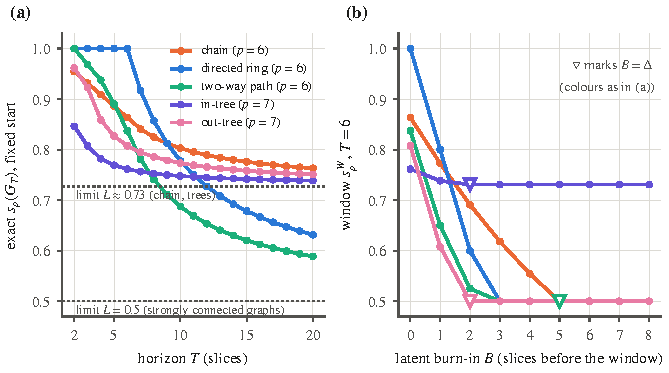
\includegraphics[width=\textwidth]{figs/fig_srho.pdf}
\caption{Exact rel-sortability of unrolled DAGs (computed by enumerating ancestors and descendants of $G_T$, not from the theorems,
which they confirm). (a) $\srho(G_T)$ under the fixed start against the horizon $T$. All curves tend to the limit of \cref{thm:limit}
(dotted: $0.73$ for the chain and the trees, $0.5$ for strongly connected graphs). The strongly connected ring has
$\srho=1$ for all $T\le p$ and the two-way path starts at $1$ and decays slowly, so strongly connected summary graphs are not
protected at short horizons. (b) The value of the last $T=6$ slices after a latent burn-in of $B$ slices: it falls to the
stationary value of \cref{thm:stat} at or before $B=\Delta$ (triangles).}
\label{fig:srho}
\end{figure}

\begin{corollary}[necessary and sufficient condition]\label{cor:iff}
$\lim_T\srho(\GT)=1/2$ iff every weakly connected component of $\GS$ is
strongly connected. Otherwise $\srho(\GT)\ge\tfrac12+\frac1{2|\Es|}$ for every
$T$. The ``if'' half is \citet[Thm.~4]{reisach2026topological}. If $\GS$ is
acyclic apart from self-loops, with $m$ other edges, $L=\tfrac12+\frac{m}{2(m+p)}$
whatever its shape (chain, in-tree, out-tree, collider).
\lean{\lname{tendsto_half_iff}, \lname{crossEdges_eq_empty_tfae}, \lname{sRho_unrolled_ge_of_cross}, \lname{reisach_theorem4}, \lname{limitValue_dag}.}
\end{corollary}

\begin{proposition}[the excess is a boundary effect]\label{prop:boundary}
For $t\ge p$, $\rho(v(t))=T\,|\rel_S(v)|-\sum_{w\in\rel_S(v)}d(\anc_S(v),w)$.
\lean{\lname{rho_unrolled_large_t}, \lname{rho_unrolled_eq}.}
\end{proposition}
So for a crossing edge with $\rel_S(i)=\rel_S(j)$ (root to child in an
out-tree, a chain), the strict order rests on $O(1)$ extra relatives out of
$\Theta(T)$, all located in the first $p$ slices. \Cref{fig:start} shows a chain of three units under both starts. A sample-based relatives count on a long record cannot see such
a difference, which motivates the stationary version.


\begin{figure}[t]
\centering
\tikzfig{fig_start}
\caption{The start artefact on the summary chain $a\to b\to c$. (a) Under the fixed start the first slice is
independent noise, so the relatives counts $\rho$ differ between a node and its child; every orange edge is oriented by the count.
(b) With a latent burn-in $B\ge\Delta$ (grey, not observed) all window nodes of a unit have the same count and the
stationary value is $\srho^W=1/2$, because a chain has a single source component (\cref{cor:statiff}). Relatives counts are computed in the full graph and
counted inside the window.}
\label{fig:start}
\end{figure}

\begin{theorem}[stationary start]\label{thm:stat}
Observe the window of the last $T\ge2$ slices of $G_{B+T}$ with a latent
burn-in $B\ge\Delta$ (or of the infinite-past graph on $V\times\mathbb Z$), with
relatives computed in the full graph. Then every window node has
$\rho_W(v(t))=T|\rel_S(v)|$, and for every $T$
\[
\srho^{W}=\tfrac12+\frac{|\Eu|}{2|\Es|},\;
\Eu=\{(i,j)\in\Es:\Src(i)\neq\Src(j)\}.
\]
\lean{\lname{rhoBurn_eq_maxFinDist}, \lname{sBurn_eq_maxFinDist}, \lname{rhoZ_eq}, \lname{sZ_eq}, \lname{relSet_eq_iff_src}; sharpness: \lname{edgeLoops_burn_sharp}.}
\end{theorem}
\emph{Sketch.} After $\Delta$ slices every finite distance is absorbed, so
$w(s)\in\rel(v(t))$ iff $\anc_S(v)\cap\anc_S(w)\ne\emptyset$. For an edge
$(i,j)$, $\rel_S(i)\subseteq\rel_S(j)$ with equality iff $\Src(i)=\Src(j)$.
This burn-in is sufficient. For one edge with self-loops ($\Delta=1$), $B=0$
leaves $\srho^W\ge2/3$ for every $T$ (Lean), and for the directed chain with
self-loops the window relatives at $B=\Delta-1$ differ from the stationary ones
at every length (\cref{prop:chainsharp}); for other graphs a shorter burn-in can
suffice (\cref{rem:sharp}).

\textbf{What is and is not claimed about sharpness.} \Cref{thm:stat} is a
sufficient condition, valid for every summary graph with self-loops. That
$\Delta-1$ does not suffice is proved, and checked in Lean, for the one-edge
graph ($\Delta=1$); it is proved on paper for the relatives of the directed
chain at every length (\cref{prop:chainsharp}, not checked in Lean), and exact
computation gives a window $\srho$ different from the stationary value at
$B=\Delta-1$ for chains with $p\le8$ and $T\le5$. For directed rings the
minimal burn-in found by computation is $\lceil\Delta/2\rceil$. For other
graphs the bound is not sharp: in 726 random summary graphs $B=\Delta$ gave
the stationary value in all of them and $B=\Delta-1$ failed in 445, so it
sufficed in 281; in a second exact computation on 396 random graphs (792
cases) none needed more than $\Delta$, the minimal burn-in equalled $\Delta$ in
51\% of the cases and was shorter by one to four slices in the rest. We have no
closed form for the minimal burn-in of a given graph.

\begin{figure}[t]
\centering
\tikzfig{fig_sharp}
\caption{Why $B=\Delta-1$ is not enough for a chain (picture of the proof of \cref{prop:chainsharp}; chain of four units, $\Delta=3$,
window of two slices). The orange node is the last unit at the first window slice; blue nodes are its ancestors.
(a) With $B=2$ latent slices no copy of $v_0$ is an ancestor, so the first-slice node of $v_0$ and the orange node
are not relatives, whereas they are under the stationary start. (b) With $B=3$ the copy of $v_0$ at slice~1 (ringed) is a
common ancestor.}
\label{fig:sharp}
\end{figure}

\begin{figure}[t]
\centering
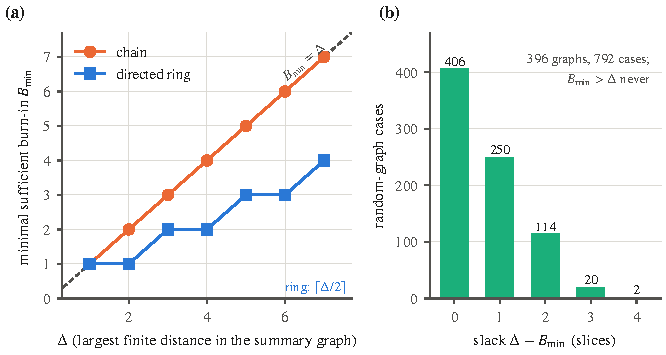
\includegraphics[width=\textwidth]{figs/fig_bmin.pdf}
\caption{The minimal sufficient burn-in $B_{\min}$ (smallest $B$ after which the window relatives counts equal their
stationary values) from exact computation (\texttt{b1y/q6\_burnin\_exact.py}, independent of the theorems; chains and rings $T=2,\dots,5$, random graphs $T\in\{3,5\}$).
(a) Directed chains need $B_{\min}=\Delta$ for every $\Delta$ computed ($1,\dots,7$); directed rings need only
$\lceil\Delta/2\rceil$. (b) For 396 random summary graphs ($792$ cases) $B_{\min}$ never exceeded $\Delta$; it equalled $\Delta$ in
$51\%$ of the cases and was shorter by one to four slices in the rest.}
\label{fig:bmin}
\end{figure}

\textbf{Scope: unit lags.} \Cref{thm:edge,thm:limit,thm:stat} are stated, and
machine-checked, for VAR(1)-shaped unrollings. If each summary edge $(i,j)$
instead acts at a lag $\tau_{ij}\in\{1,\dots,\tau_{\max}\}$ (self-loops at lag
one), the same proofs go through with $d$ replaced by the lag-weighted
distance $d_\tau$: the copy $(i(t),j(t{+}\tau_{ij}))$ is strict iff some $u$ has
$d_\tau(u,j)-\tau_{ij}+1\le t\le d_\tau(u,i)$, the limit is unchanged, and the
stationary result needs a burn-in $B\ge\Delta\tau_{\max}$ (paper proof,
\cref{app:lags}; not machine-checked). Contemporaneous (lag-0) edges are not
covered.

\begin{corollary}[stationary condition; graph classes]\label{cor:statiff}
$\srho^W=1/2$ iff every weakly connected component of $\GS$ has exactly one
source SCC. Strongly connected graphs, out-forests, chains and forks give
$1/2$. In an in-forest (a river network), $\srho^W=\tfrac12+\#\{\text{edges into
confluences}\}/(2|\Es|)$, which exceeds $1/2$ iff there is a confluence.
\lean{\lname{sBurn_eq_half_iff_maxFinDist}, \lname{sZ_eq_half_iff}, \lname{stat_half_of_outForest}, \lname{statValue_inForest}, \lname{statValue_inForest_gt_iff}, \lname{collider_stat}, \lname{fork_stat}.}
\end{corollary}


\begin{table}[t]
\caption{Rel-sortability of 3-node summary graphs (with self-loops, $|\Es|=5$).
Finite: $\lim_T\srho(\GT)$ (\cref{thm:limit}); stationary: $\srho^W$
(\cref{thm:stat}). Lean: \lname{chain3_limit}, \lname{chain3_stat},
\lname{fork_limit}, \lname{fork_stat}, \lname{collider_limit},
\lname{collider_stat}; 3-cycle by \lname{reisach_theorem4}.}
\label{tab:examples}
\centering
\setlength{\tabcolsep}{3pt}
\begin{tabular}{lcc}
\toprule
summary graph & finite $\GT$ (limit) & stationary \\
\midrule
chain $a\!\to\! b\!\to\! c$ & $0.7$ & $0.5$ \\
fork $a\!\leftarrow\! b\!\to\! c$ & $0.7$ & $0.5$ \\
collider $a\!\to\! c\!\leftarrow\! b$ & $0.7$ & $0.7$ \\
3-cycle (6 edges) & $0.5$ & $0.5$ \\
\bottomrule
\end{tabular}
\end{table}

\Cref{tab:examples} shows the two versions for 3-node graphs: chain and fork have limit $0.7$ and stationary value $0.5$, the collider $0.7$ in both. In the finite generator every
summary DAG with the same $m/p$ has the same value, so a benchmark built this
way rewards relatives-sorting on chains and forks, where the stationary
process gives no signal; for long stationary records the stationary value is
the relevant one. All statements of \cref{sec:exact} were checked by exhaustive
enumeration ($p\le4$ and $10^4$ random graphs with $p\le7$; 46{,}724 cases, 0
failures; \cref{app:enum}).

\textbf{Without self-loops} (\cref{app:noloop}). Every edge of $\GT$ still
scores $1/2$ or $1$, independently of $T$, by an explicit walk-length
criterion (machine-checked), and \citet[Thm.~4]{reisach2026topological} still
holds, but the closed form and the converse of \cref{cor:iff} fail: for the
single edge $0\to1$ without loops $\srho(\GT)=1/2$ for every $T$ (with loops
the limit is $2/3$). The loop assumption is therefore necessary for the closed
forms.

\textbf{What the value means.} Show an edge in random order with the two
relatives counts; the rule ``orient towards the larger count, flip a coin on
ties'' has accuracy exactly $\srho$, never errs on an edge it decides, and no
pairwise rule on the two counts does better (a few lines from Reisach et al.'s
Theorem~1, \cref{app:x3}). So $\srho=0.7$ caps such a method at $70\%$
orientation accuracy. Rules that also see node degrees can exceed it.
\lean{\lname{accRule_sortRule}, \lname{accRule_le_sRho}, \lname{edgeAcc_sortRule_strict}.}

\begin{remark}[random summary graphs]\label{rem:er}
For the directed Erd\H{o}s--R\'enyi summary graph $G(p,c/p)$ with a self-loop at
every node, the limits of $\srho(\GT)$ (as $T\to\infty$) and of $\srho^W$ (as
$p\to\infty$) are explicit functions of the mean degree $c$ (\cref{prop:er}).
With $x$ the largest root of $x=1-e^{-cx}$, the finite limit is
$L(c)=\tfrac12+\frac{c(1-x^2)}{2(1+c)}$; $L(1)=3/4$, and $L$ peaks at $0.754$
near $c=1.07$ and then decays like $e^{-c}$. The stationary value peaks at
$0.665$ near $c=1.09$. At $c=1$ convergence in $p$ is slow: $S=0.65574\pm0.00126$
at $p=2\cdot10^4$, $0.65784\pm0.00043$ at $2\cdot10^5$ and $0.65796$ at $10^6$,
against the formula value $0.65803$. Random summary graphs are therefore
rel-sortable only near or below criticality. The statement is proved on paper
(\cref{app:erproof}) and has not been checked by a human probabilist; Lean
covers only the deterministic witness lemmas. The statement, the figure and the
numerics are in \cref{app:er}.
\end{remark}

\subsection{With time labels the start identifies nothing more}
\label{sec:labels}

The experiments of \cref{sec:b1} hide the time labels. One may ask whether the fixed
start is also a source of information for a method that has them, for example
through the changing covariance of the transient. It is not.

\begin{proposition}[no gain from the transient]\label{prop:nogain}
Let $X_t=\mathsf BX_t+AX_{t-1}+e_t$ for $t=1,\dots,T$, with $I-\mathsf B$
invertible, $e_t$ i.i.d.\ and independent of the start $X_0\sim\nu$ ($\nu$ may
be a point mass). Put $M=(I-\mathsf B)^{-1}A$ and $\eta_t=(I-\mathsf B)^{-1}e_t$.
Then the law of $(X_0,\dots,X_T)$ depends on $(\mathsf B,A,\text{law of }e)$
only through $(M,\text{law of }\eta)$. Two structures with the same reduced
form are therefore observationally equivalent for every start law, every $T$
and every number of independent replicates. If $\Sigma_t=\mathrm{Cov}(X_t)$ is
nonsingular for some $t\le T-1$, then $M=\mathrm{Cov}(X_{t+1},X_t)\Sigma_t^{-1}$
and $\Omega=\mathrm{Cov}(\eta_t)=\Sigma_{t+1}-M\Sigma_tM^\top$ are identified.
\nolean{paper proof}
\end{proposition}
\begin{proof}
$X_t=MX_{t-1}+\eta_t$ is a Markov chain whose transition kernel depends on
$(M,\text{law of }\eta)$ only and whose initial law is $\nu$. The two formulas
follow from $\mathrm{Cov}(X_{t+1},X_t)=M\Sigma_t$ and
$\Sigma_{t+1}=M\Sigma_tM^\top+\Omega$.
\end{proof}
The covariance trajectory $\Sigma_t$ is itself a function of
$(\Sigma_0,M,\Omega)$. Identification through heteroskedasticity
\citep{rigobon2003identification} needs the \emph{innovation} covariance to
change between regimes; in a transient with fixed mechanisms only the state
covariance changes. In the lag-one model of this paper ($\mathsf B=0$) the
transition matrix is identified under either start as soon as one $\Sigma_t$
is nonsingular, in agreement with the labelled reference of \cref{sec:b1} (PCMCI+,
$\mathrm{SHD}/|E|=0.02$ under both generators). The fixed start is therefore an
artefact for label-free methods only. When each replicate is observed at a
single time, so that only the marginal laws are seen, identification of the
reduced form from these marginals has been established for linear stochastic
differential equations \citep{wang2023generator,guan2026identifying}; this is
consistent with \cref{prop:nogain} and is not our contribution.

\subsection{Is the time order identifiable without labels?}
\label{sec:ident}

\citet{reisach2026topological} end by raising the question to what extent
knowledge of the time order can and should be used for causal discovery on
independent trajectories of short time-unrolled DAGs. A prior question is how
much of the time order is hidden when the labels are removed. The statements
below are population statements with paper proofs (\cref{app:ident}); none is
machine-checked, and we do not propose a learning method.

\textbf{Setting.} The columns of the data are the $pT$ cells $(\text{unit }j,
\text{slice }t)$ of $X_{t+1}=AX_t+\varepsilon_t$ ($A_{ji}\ne0$ iff
$(i,j)\in\Es$, $\varepsilon_t$ with diagonal covariance $D$, the same $A$ and
$D$ for all $t$) in an unknown order; $p$ and $T$ are known. The \emph{column
DAG} is $\GT$ on the columns. The \emph{fixed-start law} has a diagonal
covariance of the first slice (not necessarily equal to $D$), the \emph{free
law} an arbitrary one, which covers a burn-in window and an exact stationary
start. The height of a node is one plus the number of edges of a longest
directed path ending in it. A unit is \emph{loop-only} if its only parent in
$\GS$ is itself, and \emph{isolated} if in addition it has no child other than
itself; $m_0$ is the number of loop-only units. A \emph{representation} of a
covariance $\Sigma$ is a parameter of the same model class (an assignment of
columns to cells, $A'$ with non-zero diagonal, diagonal $D'$, a start
covariance of the given law) that reproduces $\Sigma$; it is \emph{sparsest}
if no representation has fewer non-zero entries in $A'$. Markov equivalence is
equality of skeleton and unshielded colliders \citep{spirtes2000causation}.

\begin{proposition}[slices are a graph invariant]\label{prop:slices}
(a) In $\GT$, the height of $v(t)$ is $t$. Hence $T$, $p$ and the partition of
the columns into slices are determined by the column DAG.
(b) The partition of the columns into units is not: for the directed ring with
self-loops, relabelling the cell $(i,t)$ as unit $i-t \pmod p$ gives the
reversed ring with self-loops and the same column DAG.
(c) Without self-loops (a) fails: for the single edge $0\to1$ the unrolled
graph is a set of disjoint edges, and the slice of an edge is not determined.
\nolean{paper proof; (a) uses the walk-length argument behind \lname{edge_score_dist}}
\end{proposition}

\begin{proposition}[Markov equivalence class of $\GT$]\label{prop:mec}
An edge of $\GT$ is reversible within its Markov equivalence class iff it is
an edge $j(t)\to j(t{+}1)$ of the self-chain of a loop-only unit $j$. The
class has exactly $T^{m_0}$ members.
\nolean{paper proof}
\end{proposition}
So under the fixed start a perfect label-free learner that uses conditional
independence only is left with $T^{m_0}$ graphs: $m_0=0$ for a ring, $1$ for a
chain or an out-tree, and the number of leaves for an in-tree.

\begin{proposition}[fixed start, given faithfulness]\label{prop:fixident}
Let the columns be Gaussian with covariance $\Sigma$ from the fixed-start law,
$T\ge2$, and let their distribution be faithful to $\GT$.
(a) Every sparsest representation of $\Sigma$ has the true column DAG, except
that the self-chain of an isolated unit may be reversed as a whole.
(b) For $T\ge3$ the chain of an isolated unit $j$ with coefficient $a=A_{jj}$,
noise variance $d$ and start variance $v_1$ can be reversed iff its start is
stationary, $v_1(1-a^2)=d$. For $T=2$ it can always be reversed.
(c) Hence for $T\ge3$ the column DAG is identified from $\Sigma$ iff no
isolated unit has a stationary start.
\nolean{paper proof; faithfulness is assumed, not shown to be generic}
\end{proposition}

\begin{proposition}[three exact non-identifiability results]\label{prop:nonident}
(a) \emph{$T=2$, free law.} For the summary edge $a\to b$ with self-loops and a
free start covariance, the labelling with slices $\{a_1,b_2\},\{a_2,b_1\}$ is a
representation with the same number of edges and a different column DAG
($a_1\to a_2$, $a_1\to b_1$, $b_2\to b_1$).
(b) \emph{Isolated units, stationary start.} Reversing the chain of an isolated
unit with a stationary start leaves $\Sigma$ unchanged, for every $T$
\citep{weiss1975time,peters2009detecting}; in particular $p=1$ is never
identified from a stationary window.
(c) \emph{Symmetric dynamics.} If $A=A^\top$, $D=\sigma^2I$ and the start is
stationary, reversing all slices leaves $\Sigma$ unchanged for every $T$, and
the reversed column DAG is a sparsest representation.
\nolean{paper proof}
\end{proposition}

\begin{conjecture}[burn-in window]\label{conj:window}
Under the free law with $T\ge3$, $p\ge2$, a weakly connected summary graph,
faithfulness to the graph that adds a complete DAG on the first slice, and a
time-reversed innovation covariance that is not diagonal, every sparsest
representation has the true column DAG.
\end{conjecture}
We can reduce \cref{conj:window} to a finite combinatorial statement (the
skeleton admits only one partition into $T$ layers of size $p$ that is
compatible with an unrolling) and have checked it by hand only for the
summary edge $a\to b$ with $T=3$ (\cref{app:ident}).

\begin{figure}[t]
\centering
\tikzfig{fig_ident}
\caption{What is identified when the labels are hidden. (a) The height of a node in $G_T$ equals its slice, so the partition of the columns into slices is a graph invariant
(\cref{prop:slices}). (b) The Markov equivalence class of $G_T$ (\cref{prop:mec}): only the self-chain of the loop-only unit $a$ is
undirected, giving $T^{m_0}=3$ graphs; the other edges are oriented by the colliders at $b$ and $c$. (c) Without a restriction on the start
($T=2$, free start law) the same four columns admit two labellings with the same number of edges and the same law (\cref{prop:nonident}(a)): the time order is
not identified.}
\label{fig:ident}
\end{figure}

\textbf{Reading.} Under the fixed start, hiding the labels hides little in
the population: the slices are a graph invariant, and the column DAG is
identified up to isolated units. This is a third regularity of the
time-unrolled construction, next to rel- and var-sortability, and unlike them
it comes from the shape constraint (the graph is an unrolling), which a burn-in
does not remove; whether it also survives a burn-in is \cref{conj:window}.
Three cautions apply. The statements assume faithfulness, and the tied
parameters of an unrolled model form a null set among all linear Gaussian
models on $\GT$, so the usual genericity argument does not apply directly.
For coloured Gaussian DAG models \citet{boege2025colored} prove that a generic
covariance matrix is faithful when only edges or only vertices are coloured,
and give a mixed example that has no faithful distribution; which coloured DAGs
admit one is open (\cref{sec:rw-ident}). Our model ties both transition weights
and, if the noise variances are equal across slices, noise variances, so on our
reading it is the mixed case, and we have not established faithfulness for it.
The statements concern the global optimum of a sparsity criterion, not a
computable procedure. And they say nothing about finite
samples: at $n=1000$ FLOP is far from the labelled reference
(\cref{tab:b1x}). Dynamic Bayesian networks with a start network and a tied
transition network are classical when the labels are known
\citep{friedman1998learning}.

\subsection{Machine-checked proofs}
\label{sec:lean}

The formalisation (Lean~4, \citealp{demoura2021lean4}, with Mathlib,
\citealp{mathlib2020}; 16 files, 4{,}159 lines, clean rebuild of the final
state) certifies the exact and stationary results of \cref{sec:exact}
(\cref{thm:edge,thm:limit,thm:stat}, \cref{cor:iff,cor:statiff},
\cref{prop:boundary}), including the $\Delta$ forms of the bound and the
burn-in and the sharpness example of \cref{rem:sharp} (one edge, $\Delta=1$),
the loop-free exact edge value and the accuracy reading, the algebra of the
real-data estimand $\tilde s$ (\cref{app:estimand}), and the deterministic
algebra of F1--F3. It does \emph{not} certify the ER limits, the loop-free
limit and periodicity, the lag-weighted extension, the statements of
\cref{sec:labels,sec:ident}, or any probability bound or limit theorem. The
sources contain 259 theorem and lemma declarations and no \texttt{sorry},
\texttt{admit} or \texttt{axiom}. The axiom report, produced with
\texttt{\#print axioms}, lists 163 of them (33 headline theorems, 53 graph
lemmas, 65 algebraic facts, many elementary, and 12 examples: concrete graphs, the
one-edge sharpness example and one numerical instance), each depending only on \texttt{propext},
\texttt{Classical.choice} and \texttt{Quot.sound}; the other 97 theorem and
lemma declarations are not in the report. Relatives, $\srho$, $\GT$ and the windows are defined from scratch
following \citet{reisach2026topological}. No human has yet checked that each
Lean statement matches its paper statement, and \emph{machine-checked} in this
paper means a theorem proved in Lean for the statement as formalised.
\Cref{app:lean} maps every statement to its Lean names and status.

\textbf{Takeaway (Q1, Q2).} The footprint is a function of the summary graph
alone. Its exact value, its limit and the burn-in after which it no longer
depends on the start are settled for lag-one unrollings with self-loops, with
the graph statements checked in Lean. Without labels the slices remain
identifiable under a fixed start, conditional on faithfulness. The
distributional side of the start (variances, correlations) is not covered by
these results.

%=============================================================================
\section{Finite Samples: How Much of the Footprint an Estimator Sees}
\label{sec:finsamp}

\textbf{Question (Q3).} How much of the footprint can an estimator see? The
exact values are population statements about a graph.
\Cref{sec:finite} asks whether the relatives behind them can be estimated from
one finite, autocorrelated record, and \cref{sec:agg} asks what block means and
subsamples of a faster process do to the three sortability criteria.

\subsection{Estimating relatives from one record}
\label{sec:finite}

We now ask whether the population relatives can be estimated. $X$ is a
zero-mean stationary Gaussian process with absolutely summable auto- and
cross-covariances $\gamma_{ab}(h)$, standardised so that $\gamma_{aa}(0)=1$,
observed at $n$ times. Two nodes are declared relatives if the Fisher-$z$ test
of the sample correlation $\hat r_{ab}$ rejects at level $\alpha$ with
Bonferroni over $m=d(d{-}1)/2$ pairs, i.e. $|\hat r_{ab}|>\tanh(z_c/\sqrt{n'-3})$,
$z_c=\Phi^{-1}(1-\alpha/2m)$; $\hat\rho(v)=1+\#$declared partners. The
\emph{nominal} test uses $n'=n$. Let
$B_{ab}=\sum_h|\gamma_{aa}(h)\gamma_{bb}(h)+\gamma_{ab}(h)\gamma_{ab}(-h)|$
(for an independent pair $B_{ab}=\sum_h|\rho_a(h)\rho_b(h)|$, at least the
Bartlett sum $W_{ab}=\sum_h\rho_a(h)\rho_b(h)$, with equality iff all products
are nonnegative; e.g.\ $4.56$ against $0.22$ for AR(1) coefficients $0.8$ and
$-0.8$).

\textbf{F1: recovery and effective sample size.} That the nominal-$n$ test has
the wrong size under autocorrelation is classical: effective degrees of
freedom go back to \citet{bartlett1935}, with spatial and multivariate versions
in \citet{clifford1989} and \citet{roy1989}, and the variance with exactly our
summand $B_{ab}$ is in \citet{afyouni2019effective}. We add a non-asymptotic
exact-recovery bound for the relatives set (\cref{thm:f1}, \cref{app:finite}):
if the thresholds separate the population correlations by more than explicit
deviations, the declared set and hence $\hat s=\srho^{\mathrm{pop}}$ are
recovered with failure probability decaying as
$\exp(-n\min(\tau,\rho_{\min}-\tau)^2/(2(\sqrt B+\rho_{\max}\sqrt{D_\gamma})^2))$,
so $n/B$ acts as an effective sample size. For i.i.d.\ snapshots $B=1+\rho^2$;
under strong persistence $B$ can be in the tens. This bound is for a fixed
threshold; for the Bonferroni Fisher-$z$ threshold $\tau_n\asymp z_c/\sqrt{n'}$
that we use, the failure probability it certifies tends to
$d(d{-}1)e^{-z_c^2/(2B)}>0$ ($0.089$ for i.i.d.\ data, $d=5$, $\alpha=0.01$;
\cref{prop:f1scope}), and recovery is instead guaranteed asymptotically
(\cref{prop:plugin}).

\begin{proposition}[size distortion of the nominal test]\label{prop:nominal}
In this setting, a non-relative pair is declared by the nominal test with
probability $\to2\bar\Phi(z_c/\sqrt{W_{ab}})$, $W_{ab}=\sum_h\gamma_{aa}(h)\gamma_{bb}(h)$
($\le B_{ab}$, with equality iff all products are nonnegative), above the nominal $\alpha/m$ when $W_{ab}>1$. With
$\neff=n(1-\rho^2)^2/W_{ab}$ ($W$ the delta-method Bartlett variance) the
false-positive rate tends to $\alpha/m$.
\nolean{uses the multivariate Breuer--Major theorem}
\end{proposition}
The joint asymptotic normality used here follows from the multivariate
Breuer--Major theorem \citep{arcones1994limit,nourdin2011quantitative}
(\cref{app:finite}). On real data
$\neff$ is estimated by $n/\hat B_{ab}$,
$\hat B_{ab}=\max(1,1+2\sum_{h=1}^{K}\hat\rho_a(h)\hat\rho_b(h))$. If
$K=K_n\to\infty$ with $K_n=o(n)$, $\hat B_{ab}$ is consistent, the plug-in test
has asymptotic size at most $\alpha/m$ per pair, and the relatives set is
recovered with probability at least $1-\alpha$ in the limit
(\cref{prop:plugin}). Our code uses a fixed $K$ ($20$--$100$), which controls
size only if the truncated sum captures the Bartlett sum: at AR coefficient
$0.99$ and $K=50$ the size is $0.113$ against $0.05$, while on the B3 data
$K$ up to $300$ changes none of 2{,}730 pair decisions (\cref{app:finite}). We
did not run this check on the river data, which are the most persistent, or
on study~3 and E1. For linear
processes with non-Gaussian i.i.d.\ innovations the null variance, and hence
the size results, are unchanged, because independent series share no fourth
cumulant; for relatives the variance changes, which affects power but not the
limits (\cref{rem:nongauss}).

\begin{figure}[t]
\centering
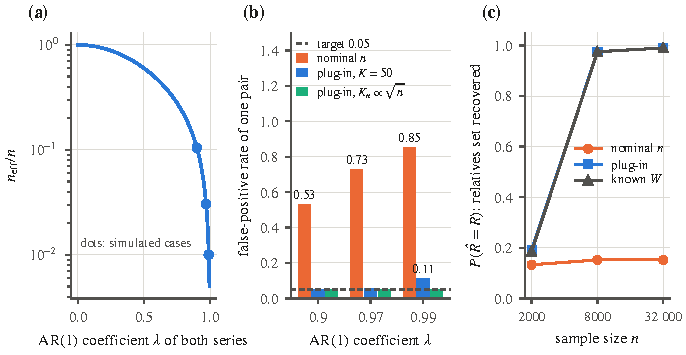
\includegraphics[width=\textwidth]{figs/fig_finite.pdf}
\caption{Estimating relatives from one autocorrelated record (simulations of \texttt{finite2/sim\_finite2.py}, fixed seeds).
(a) The effective sample size $n_{\mathrm{eff}}=n/W$ of the correlation of two independent AR(1) series with the same coefficient $\lambda$, with
$W=(1+\lambda^2)/(1-\lambda^2)$; dots are the simulated cases. (b) False-positive rate of one non-relative pair at nominal level $0.05$:
the test that uses $n$ rejects far too often, the plug-in test that estimates $W$ is close to the target, except that a fixed truncation lag $K=50$ is too
short at $\lambda=0.99$ ($0.11$). (c) Probability that the Bonferroni Fisher-$z$ procedure recovers the relatives set of a five-node graph
($\lambda=0.9$, $\alpha=0.05$): the nominal test does not, the plug-in test does, and it behaves like the test that knows $W$.}
\label{fig:finite}
\end{figure}

\textbf{F2: saturation by a latent driver.} Let $X_v=Y_v+b_vC$ with $C$ a
stationary unit-variance process independent of the VAR $Y$, and
$\ell_v=b_v^2/\mathrm{Var}X_v$ the driver's share of variance.

\begin{proposition}[saturation]\label{prop:f2}
For summary non-relatives,
$\rho_{uv}=\mathrm{sgn}(b_ub_v)\sqrt{\ell_u\ell_v}=:\kappa_{uv}$. If all $b_v\ne0$,
every pair is a population relative and the population rel-sortability is
exactly $1/2$; $P(\hat s_n\ne\frac12)\le(d^2{+}3d)e^{-cn}$ with
$c\approx\kappa_{\min}^2/(18(\sqrt B+\sqrt{D_\gamma})^2)$. Asymptotically, a pair is
detected with probability $>1/2$ once
$n>\nhalf=3+(z_c/\atanh\kappa)^2\approx z_c^2/\ell^2$ (nominal test; for the
effective test, the same bound on $\neff$).
\lean{\lname{prop21_corr_std}, \lname{sOf_saturated}, \lname{abs_sOf_sub_half_le}, location of $\nhalf$: \lname{ncrit_eq_iff}; the probability statements are not machine-checked.}
\end{proposition}
$\nhalf$ does not depend on autocorrelation, which only sets the width of the
transition. A driver with share $\ell=0.1$ saturates at $n\approx10^3$, and
one with $\ell=0.64$ at $n\approx22$ (both for $z_c=3.29$). A relatives count on a long record can
recover the summary relatives only while
$\max_{\text{non-rel}}|\kappa|<\tau_n<\min_{\text{rel}}|\rho|$, a window that
closes at $n$ of order $\nhalf$.

\textbf{F3: conditioning on a proxy.} A natural remedy is to condition on a
measured proxy $Z$ of the driver. It works only if the proxy is almost
perfectly reliable.

\begin{proposition}[conditioning]\label{prop:f3}
Let $Z=\sqrt r\,C+\sqrt{1-r}\,e$ with reliability $r=\mathrm{corr}(Z,C)^2$,
$\pi_{uv}$ the partial correlation given $Z$, and $\rho^Y$ the driver-free
correlation. Then
\[
\pi_{uv}=\frac{\rho^Y_{uv}\sqrt{(1{-}\ell_u)(1{-}\ell_v)}+(1{-}r)\,\mathrm{sgn}(b_ub_v)\sqrt{\ell_u\ell_v}}{\sqrt{(1-r\ell_u)(1-r\ell_v)}} .
\]
At $r=1$ the conditional relatives are the summary relatives and
\cref{thm:stat} is restored. For non-relatives with $\ell_u,\ell_v\in(0,1)$ and
$b_ub_v\ne0$, $|\pi_{uv}|$ is strictly decreasing in $r$ and vanishes only at
$r=1$; fewer than half of the non-relative pairs are declared only if
$r>r_{\mathrm{crit}}=1-\frac{\tau'(1-\ell)}{\ell(1-\tau')}$,
$\tau'=\tanh(z_c/\sqrt{n'-4})$ (equal shares). If the driver reaches nodes
through different filters, a scalar proxy leaves a nonzero residual even at
$r=1$. The reliability is identified by $\rho_{uZ}\rho_{vZ}/\rho_{uv}=r$, the
identity behind the three-indicator identification rule for one-factor models
\citep[Ch.~7]{bollen1989structural}.
\lean{\lname{prop31_std}, \lname{cor32}, \lname{absPi_strictAntiOn}, \lname{absPi_eq_zero_iff}, \lname{rcrit_iff}, \lname{thm35_bracket}, \lname{pc_lipschitz}, \lname{prop36_ar1_ne_zero}, \lname{prop36_rank_one}, \lname{prop38_ratio}.}
\end{proposition}
So spurious conditional relatives appear for every $r<1$ once $n$ is large;
$r_{\mathrm{crit}}=0.95$ for $\ell=0.64$ and $\tau'=0.082$. Formalisation found
four missing nondegeneracy hypotheses in our earlier statements (e.g.\
$b_ub_v\ne0$; \cref{app:lean}). The algebra of F2 and F3 is machine-checked;
the probability statements are not. The non-asymptotic bounds are loose
(factors 3--13 in $n$, \cref{app:sims}); the asymptotic statements matched
every simulation to within $0.03$ and are the ones used in \cref{sec:real}.

\textbf{Detectability as the second factor.} The statements above separate two
things that the exact values of \cref{sec:theory} run together. The graph
decides which pairs are relatives; the sample size, the autocorrelation and any
latent driver decide which relatives a test can detect. An estimator sees the
footprint only through the second. In the benchmark experiment of
\cref{sec:b1} this shows up as follows: the exact gap between the two starts
orders the simulated conditions, and a post hoc calculation of which
correlations are detectable at $n=1000$ reproduces the size of the observed
gain. That calculation is the analytic expectation of the algorithm, so it
checks consistency of size and does not separate the graph mechanism from a
general change in correlation strength. A designed test does
(\cref{sec:controls}): the share of the exact gap that is realised rises from
$0.18$ at $n=200$ to $0.76$ at $n=25{,}000$, and from $0.09$ to $0.51$ when the
spectral-radius cap rises from $0.5$ to $0.95$; and a start that has the
population relatives of a burn-in but the detectable correlations of the fixed
start keeps $0.96$ of the gain.

\subsection{Block means and subsamples}
\label{sec:agg}

Real records are often block means or subsamples of a faster process. For a
stable linear SVAR with independent innovations, nodes with disjoint summary
ancestor sets are independent at all lags, and so are any per-node,
time-invariant transforms of them, block means and subsamples included;
otherwise the lag-0 covariance is nonzero for almost every parameter
(\cref{prop:zero}). So the population relatives of contemporaneous values are
$\rel_S$ for every observation scheme, and the population relatives sort takes
the stationary value of \cref{thm:stat} (on non-self-loop edges), not the
finite-$\GT$ value. Var- and $R^2$-sortability behave differently
(\cref{thm:agg}): block means converge to the long-run structural model, whereas
subsamples keep the snapshot covariance, so for large blocks block-mean
$R^2$-sortability is $0$ on out-stars and $1$ on in-stars with at least two
arms. Subsampling also changes which structures are identifiable
\citep{gong2015subsampled,hyttinen2016subsampled}; we ask only about the three
criteria. The statements, the numerical observations and the proofs are in
\cref{app:aggstate,app:agg}.

\textbf{Takeaway (Q3).} Relatives can be estimated from one record only while
the effective sample size is above the saturation threshold of a latent driver
and the true relatives are detectable at lag zero; under those conditions the
population statement is recovered with probability of at least $1-\alpha$ in the
limit (\cref{prop:plugin}), and outside them the count carries little or no
information. The bounds are loose,
the proofs are on paper, and block means and subsamples change var- and
$R^2$-sortability while leaving the population relatives unchanged. In the
benchmark simulations, the effect of the start on a relatives sort is the
detectable image of the exact gap (\cref{sec:controls}).

%=============================================================================
\section{Experiments and Real-Data Evidence}
\label{sec:experiments}

\textbf{Question (Q2 empirically, and Q4).} What does the start of a simulation
do to what label-free learners appear to achieve, and does a relatives count
orient edges in real records? \Cref{sec:b1} measures what the start does to
benchmark results when the time labels are hidden from static learners.
\Cref{sec:controls} reports controlled tests of two readings that
\cref{sec:b1} leaves open: what carries the effect of the start, and whether the
learner reversal survives tuning and a variance control.
\Cref{sec:real} applies the finite-sample theory and the criterion to real
records, which is a different question: whether relatives can be estimated from
one record at all.

\begin{figure}[t]
\centering
\tikzfig{fig_pipeline}
\caption{The experimental pipeline and where the four questions enter. A summary graph is simulated under a start rule (fixed start or
latent burn-in), the time labels are dropped and the columns shuffled, a learner returns a graph, and the result is scored against the
window DAG $G_T$. Edges that leave the first slice are scored separately in the controlled tests, because under a burn-in their
confounder lies in the unobserved past.}
\label{fig:pipeline}
\end{figure}

\subsection{The start artefact in simulated benchmarks}
\label{sec:b1}
\label{sec:b1exp}

\textbf{Design (B1).} We unrolled 420 summary graphs (30 per family and
$p\in\{5,10\}$; families in \cref{tab:b1}; details in \cref{app:b1}) over $T\in\{3,5,10\}$ and drew
$n=1000$ linear-Gaussian trajectories (positive weights, heterogeneous noise)
either with a fixed start (G1: the first slice is pure noise, which is what
unrolling from $t=1$ gives; the preprint of \citealt{reisach2026topological}
fixes no initial law) or after a latent burn-in of 100 steps (G2; an exact stationary start reproduced G2 to
within $0.013$). Methods saw the $pT$ columns shuffled, with time labels
hidden: rel-, $R^2$- and Var-SortnRegress
\citep{reisach2026topological,reisach2023scale}, FLOP
\citep{wienobst2026flop}, PC \citep{spirtes2000causation} in causal-learn
\citep{zheng2024causallearn} and a random order; SID by gadjid
\citep{henckel2024gadjid}. The analysis plan was committed before any
algorithm was run (\cref{app:b1}). Weights were drawn uniformly from
$[0.5,1]$ on every summary edge and rescaled to a spectral radius of at most
$0.8$; the realised radii were not tabulated, and persistent dynamics near a
unit root are not covered. CIs below resample whole summary graphs.

\begin{table}[t]
\caption{B1, heterogeneous noise, raw data; means over 180 data sets per
family. OA: order accuracy of rel- and Var-SortnRegress, G1 / G2. $\Delta$OA:
G1$-$G2 for rel, with 95\% graph-cluster bootstrap CI. SC: strongly connected.}
\label{tab:b1}
\centering\setlength{\tabcolsep}{3pt}
\begin{tabular}{lcccc}
\toprule
family & exact $\srho$ & rel OA & $\Delta$OA rel & var OA\\
\midrule
symER (SC) & .78/.50 & .63/.50 & $+.126$ [.115,.137] & .64/.50\\
ring (SC)  & .95/.50 & .69/.51 & $+.180$ [.167,.193] & .73/.50\\
chain      & .89/.50 & .75/.53 & $+.217$ [.209,.226] & .93/.70\\
out-tree   & .84/.50 & .69/.55 & $+.144$ [.127,.161] & .94/.71\\
in-tree    & .79/.66 & .74/.67 & $+.069$ [.057,.081] & .95/.72\\
ER($c{=}1$)& .77/.56 & .67/.59 & $+.085$ [.068,.103] & .86/.65\\
ER($c{=}2$)& .83/.52 & .70/.59 & $+.109$ [.092,.127] & .74/.59\\
\bottomrule
\end{tabular}
\end{table}

\textbf{Rel-sortability: what the exact values do and do not explain.} The
fixed start raised rel-SortnRegress order accuracy in all five
non-strongly-connected families (pooled over these five $+0.125$, 95\% CI
$[0.116,0.134]$; Holm $p\le1.1\cdot10^{-10}$ per family; $+0.133$ over all
seven). Because this order accuracy is essentially the estimated
rel-sortability, the hypothesis tests whether estimated counts follow the exact
values, not algorithm impact. Agreement in sign is not a discriminating test:
all 42 (family, $p$, $T$) cells have a positive exact gap
$\srho(\GT)-\srho^W$ and a positive observed gain. What the exact gap adds is a
ranking and a rough scale: Spearman $0.80$ across the 42 cells (graph-cluster
permutation $p\le10^{-4}$; $0.62$ over graph--horizon units) and slope $0.53$,
so the observed gain is about half the exact gap. A post hoc calculation
(\cref{fig:oracle}, \cref{app:b1x}) reproduces the size: the expected outcome
of the same thresholded-correlation sort under the exact start-dependent
window covariances, with the probability that each correlation is detected at
$n=1000$, matches the gain with cell $R^2=0.97$ and slope $1.03$. This is the
analytic expectation of the algorithm, so it checks that the simulated gain
has the size its covariances imply. It does not separate the structural
mechanism of \cref{sec:exact} (pairs that are relatives under one start only)
from a general change of correlation strength during the transient. In a
joint regression the exact gap adds nothing to it (coefficient $-0.063$ over
cells and $-0.039$ over graph--horizon units). For rings with $p=T=10$, for
example, the gap is $0.50$ but only $40\%$ of the relatives have a detectable
correlation; the calculation gives $+0.094$ and we observed $+0.079$. The designed
test that separates these readings is reported in \cref{sec:controls}. The gain
does not come from the latently confounded first window slice: without edges
leaving it, it is $+0.089$ $[0.079,0.100]$. Strong connectivity did not protect
short horizons: on rings and symmetrised ER graphs the gain was $+0.13$ to
$+0.31$ in all six cells with $T<p$ and $+0.08$ to $+0.22$ in four of the six
cells with $T\ge p$, consistent with the exact values (rings: $\srho(\GT)=1$
for $T\le p$). A separately planned replication (B1-NL, \cref{app:b1nl}; new
seeds) with nonlinear additive dynamics, signed weights, and signed weights
with uniform noise reproduced the gain in all 126 cells (pooled $+0.108$,
$+0.137$, $+0.137$; 5/5 families significant in each; Spearman $0.68$--$0.82$,
slopes $0.34$--$0.56$).

\begin{figure}[t]
\centering
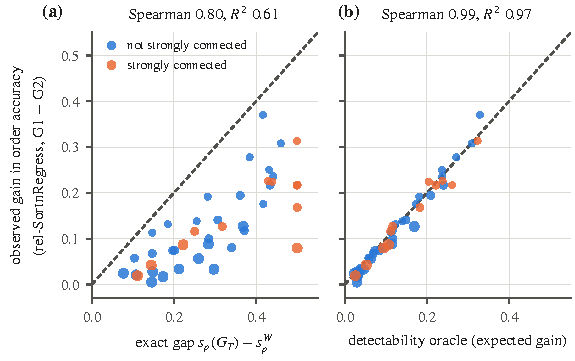
\includegraphics[width=0.8\textwidth]{figs/fig_oracle.pdf}
\caption{B1: observed G1$-$G2 gain in rel-SortnRegress order accuracy per
(family, $p$, $T$) cell (marker size grows with $T$; squares: strongly
connected) against the exact population gap (left) and against the post hoc
expectation of the algorithm under the exact window covariances (right).
Dotted: identity.}
\label{fig:oracle}
\end{figure}

\textbf{Sort-based baselines.} The start changed the size of most method
differences (Holm-significant G1$\times$G2 interactions in 294 of 595
pair$\times$cell SHD tests) and flipped the sign of 11 (Holm over 1{,}190
tests), all among sort-based baselines: e.g.\ on chains rel-SortnRegress beat
$R^2$-SortnRegress under G1 and lost under G2. These baselines are no better
than the empty graph on SHD under G2 ($\mathrm{SHD}/|E|=1.39$--$2.04$; FLOP
$0.46$ and PC $0.64$ never exceed $1$), so SID is the more informative metric
for them. In B1-NL the swap hypothesis was supported by the plan's rule under
nonlinear dynamics, but only through one swap between two weak baselines, and
not under signed weights; we discount it. The interactions themselves
replicate (in-tree Var-SortnRegress vs FLOP on SHD, SID and orientation in all
three parametrisations; chain rel- vs $R^2$-SortnRegress on SID and
orientation, and on SHD in the short-horizon cells); sign reversals on SHD did
not recur because the B1-NL level differences are larger.

\textbf{Competitive learners: the second artefact.} The fixed start also
makes the window var-sortable, because variance accumulates from the
noise-only first slice (Var-SortnRegress $+0.20$ raw, $+0.002$ standardised;
rel-SortnRegress is scale invariant). A third planned experiment
(\cref{app:b1x}; 384 new data sets, families ring, chain, in-tree, ER($c{=}2$),
$T\in\{3,5\}$) ran DAGMA \citep{bello2022dagma}, NOTEARS
\citep{zheng2018notears} and GOLEM \citep{ng2020golem} with default settings on
raw and standardised data (\cref{tab:b1x}). On raw data all four variants
improved sharply under G1 (order accuracy $+0.16$ to $+0.23$, SHD$/|E|$ $-0.41$
to $-0.55$; Holm $\le4\cdot10^{-8}$). This
changed their ranking against FLOP: on in-trees DAGMA and NOTEARS beat FLOP
under G1 and lost under G2 (both reversals Holm-significant and repeated on
SID and order accuracy; DAGMA's also with first-slice pairs excluded; GOLEM
only drew level with FLOP under G1), and a continuous method had the lowest
mean SHD$/|E|$ among label-free methods in 3 of 8 (family, $p$) cells under G1
(one of them by $0.09$ against $0.10$, untested) against 0 of 8 under G2. The
plan had predicted no rank change against FLOP; that prediction failed. It
had predicted that standardisation would reduce the gain without removing it.
By the plan's rule this held, except that DAGMA's SHD gain was removed; but
the order-accuracy effect of the start became negative for DAGMA and GOLEM
($-0.06$ to $-0.10$), which the plan had not expected, and NOTEARS kept a small
significant gain ($+0.036$; SHD$/|E|$ $-0.077$). At the time of this experiment we could only suspect var-sortability:
standardised DAGMA and GOLEM are below chance in order accuracy under both
starts ($0.31$--$0.42$), so they cannot show whether a scale-free part remains;
standardised NOTEARS shows that some does; the fixed start also raises
$R^2$-sortability, which is scale free; and the var-sortability gain is the same
on rings and chains while the learners' gains are not. The variance-matched
control and the tuned re-run were planned after this experiment and are reported
in \cref{sec:controls}. In
any case \cref{thm:limit,thm:stat} do not predict these ranking changes; they
cover the scale-free gain of the sort baselines (rel-SortnRegress $+0.19$
again here). PCMCI+ \citep{runge2020pcmciplus}, which uses the time labels,
recovers the window under both generators ($\mathrm{SHD}/|E|=0.02$).
Holm across the 21 claim-level tests of B1, B1-NL, B3 and this experiment
keeps every claim except the B1-NL swap claim under signed weights ($p=0.108$).
The claim-level p-values were computed after the fact, the sequence of studies
was adaptive, and the correction does not cover the real-data tests of
\cref{sec:real}.

\begin{table}[t]
\caption{Competitive learners (\cref{app:b1x}), raw data unless noted; 96
graphs, G1 / G2. OA: ancestral order accuracy; $\Delta$: G1$-$G2 with
graph-cluster 95\% CI. GOLEM-NV at $p=5$ only.}
\label{tab:b1x}
\centering\setlength{\tabcolsep}{2.5pt}
\begin{tabular}{lccc}
\toprule
method & SHD$/|E|$ & OA & $\Delta$OA \\
\midrule
FLOP & .19 / .52 & .89 / .77 & -- \\
DAGMA & .35 / .90 & .80 / .60 & $+.197$ [.177,.216] \\
NOTEARS & .47 / .89 & .74 / .59 & $+.156$ [.136,.175] \\
GOLEM-NV & .39 / .80 & .79 / .56 & $+.232$ [.205,.258] \\
DAGMA, std. & .87 / .87 & .35 / .41 & $-.064$ [$-$.079,$-$.048] \\
NOTEARS, std. & .76 / .84 & .49 / .46 & $+.036$ [.022,.049] \\
in-trees: DAGMA & .08 / .87 & & \\
\quad NOTEARS / FLOP & .13 / .76; .30 / .56 & & \\
PCMCI+ (labels) & .02 / .02 & 1.0 / 1.0 & -- \\
\bottomrule
\end{tabular}
\end{table}

\textbf{Which generators are exposed.} Two conditions are needed. First, the
slices must be given to a method that does not use time order; a single
record given to a time-series method is outside this threat model. Second,
the start must matter: for the graph artefact of \cref{sec:exact} this means
a burn-in shorter than $\Delta\tau_{\max}$ steps, and for the variance
artefact it means a start that has not mixed in distribution, which depends on
the spectral radius and which we did not compute for any deployed generator.
We read the source code of common time-series generators (\cref{app:b1x}).
The time-unrolled construction of \citet{reisach2026topological} meets both
conditions: it starts at $t=1$ with no burn-in and gives every slice to the
method as a separate variable (its data code is not public). The others
produce one record for time-series methods, so they fail the first condition
as shipped. On the second: an exact stationary start
\citep{herman2025unitless} removes both artefacts; burn-ins of 100 to 1000
steps (causalnex, the Neural-GC simulators \citep{tank2021neural}) remove the
graph artefact and the variance artefact only if the process mixes within
them; tigramite's \texttt{structural\_causal\_process} \citep{tigramite} drops
$\lfloor0.2T\rfloor$ steps, its older \texttt{var\_process} none, the CDML
generator \citep{lawrence2021dgp} $2\tau_{\max}$, and CausalTime's demo rolls
out 20 steps \citep{cheng2024causaltime}, so windows cut from their first
steps would be exposed. We could not check how the CauseMe data were
initialised.

\subsection{Controlled tests of the two-factor reading and of the learner reversal}
\label{sec:controls}

\textbf{Question.} Which part of the start artefact is carried by the
population relatives pattern and which by the correlations that a test can
detect, and does the learner reversal survive tuning and a variance control?
\textbf{Plan.} A time-stamped plan (\cref{app:b1y}) fixed designs, thresholds,
seeds, a table that maps outcomes to the paper's reading, and a multiplicity
family before any data were simulated. Its two addenda (the second restricts
NOTEARS to $d\le30$ after fit times were measured) were committed before the
scored runs they govern. In this subsection all metrics drop the edges that
leave the first slice (SHD$_{x1}$, OA$_{x1}$): under a latent burn-in the first
window slice is confounded by the last burn-in slice and its pairs are scored
differently (reference SHD $0.044$ under the fixed start and $0.273$ after a
burn-in, but $0.041$ against $0.048$ without first-slice pairs). Units are
summary graphs, and intervals are graph-cluster bootstrap intervals.

\textbf{Matched-correlation counterfactual.} For the same graphs, weights and
noise (300 graphs that are not strongly connected, $T\in\{3,5,10\}$) only the
covariance of the first slice was changed. The counterfactual CF1 keeps the
population relatives of the fixed start and rescales the first slice by a
factor $c\in\{0.25,\dots,4\}$. The counterfactual CF2 has the population
relatives of the burn-in, hence the same exact $\srho$, but in its smallest
setting every new correlation is below half the detection threshold, so that
the pairs a test can detect are those of the fixed start; larger settings make
the burn-in pattern detectable. A second independent draw of the fixed start is
the negative control. The control was valid ($-0.004$ [$-0.011,+0.002$]; limit
$\pm0.01$), and the burn-in was mixed (exact stationary start within $0.001$).
The fixed start raised the order accuracy of rel-SortnRegress by $+0.090$
[$0.080,0.101$]. CF2 with undetectable burn-in correlations kept $0.955$
[$0.884,1.030$] of this gain; where the burn-in pattern became detectable the
retention fell to $0.92$ and $0.79$. Changing the strength at the fixed start's
own pattern moved the gain by $0.008$ [$0.001,0.016$] between the weakest and
the strongest setting, which the plan's rule (a quarter of the gain) calls
flat. By the plan's rule the first result reads ``detectable strength, not
population pattern'': the order accuracy of the relatives sort responds to
which pairs clear the detection threshold, not to the population relatives
pattern itself.

\begin{figure}[t]
\centering
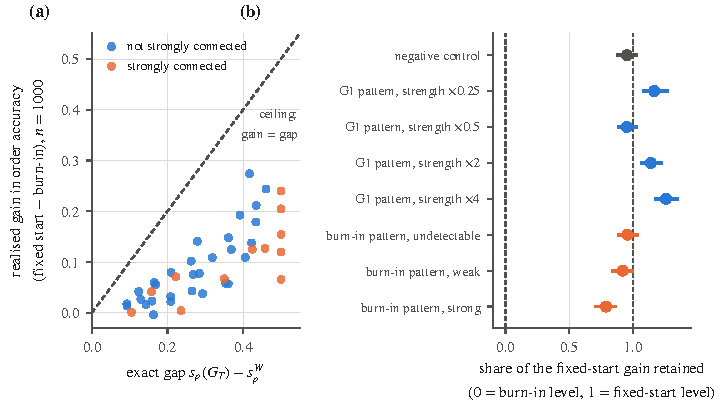
\includegraphics[width=\textwidth]{figs/fig_controls.pdf}
\caption{Matched-correlation counterfactual (\texttt{b1y/results/q1.csv.gz}; graphs that are not strongly connected unless marked;
order accuracy without first-slice edges). (a) Each point is one (family, $p$, $T$) cell: the realised gain of the fixed start over a burn-in,
$n=1000$, against the exact gap of \cref{thm:limit,thm:stat}. All cells lie below the line gain = gap. (b) Share of the fixed-start gain
retained when only the first-slice covariance is changed (graph-cluster 95\% intervals). Data with the fixed start's population pattern keep the gain at every
strength. Data with the burn-in's population pattern keep it ($0.96$) while the new correlations are below the detection threshold and keep less of it ($0.92$, $0.79$) as they become detectable.}
\label{fig:controls}
\end{figure}

\textbf{Dose.} On rings, chains and ER($c{=}2$) graphs the share $Q(n)$ of the
exact gap that is realised was $0.18$, $0.40$, $0.57$ and $0.76$ at
$n=200$, $1000$, $5000$ and $25{,}000$ ($+0.36$ [$0.29,0.43$] between $1000$
and $25{,}000$), and $0.09$ and $0.51$ at spectral-radius caps $0.5$ and
$0.95$ (difference $+0.42$ [$0.35,0.49$]). In the main design (graphs that
are not strongly connected, $n=1000$) the within-family slope of the gain on the
exact gap was $0.57$ [$0.40,0.73$], against $0.53$ pooled in B1. Read together: the exact gap is the large-sample ceiling of what the start
does to the relatives sort, and the effect realised at a finite $n$ is its
detectable image, which grows with $n$ and with the correlation strength that
the spectral radius sets. The share had not reached one at $n=25{,}000$.

\begin{figure}[t]
\centering
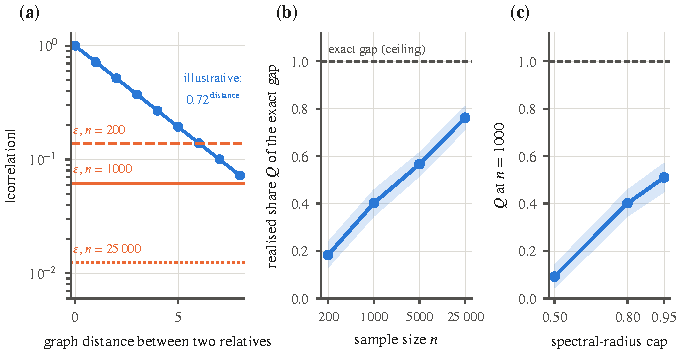
\includegraphics[width=\textwidth]{figs/fig_twofactor.pdf}
\caption{Two factors behind the effect of the start. (a) Illustration (not data): the correlation between two relatives decays with their graph distance,
and a pair is detected only if it clears the threshold $\varepsilon(n)$, which falls as $n$ grows, so more of the exact footprint is visible at large $n$.
(b) The share $Q$ of the exact gap that is realised in the order accuracy of the relatives sort, against $n$ (rings, chains, ER($c{=}2$); graph-cluster
95\% bands). (c) The same share at $n=1000$ against the spectral-radius cap of the weights: stronger dynamics make more relatives detectable.
$Q$ stays below one at $n=25\,000$.}
\label{fig:twofactor}
\end{figure}

\textbf{Learner reversal.} We used chains, in-trees, rings and ER($c{=}2$)
graphs in six $(p,T)$ cells with $d$ from $15$ to $60$ and 12 graphs per
(family, $p$). DAGMA and NOTEARS hyper-parameters were chosen on separate
validation seeds, pooled over both starts so that tuning could not favour the
artefact; GOLEM-EV and GOLEM-NV ran at their defaults ($d\le50$), and NOTEARS
only for $d\le30$ because fits on burn-in data were too slow in larger cells.
Two further arms rescaled each data set so that its marginal variances equal
those of the other start, leaving correlations unchanged; the manipulation
check passed (order accuracy of Var-SortnRegress within $0.01$ of the target
start). On in-trees, tuned DAGMA, NOTEARS and GOLEM-NV beat FLOP under the
fixed start and lost to it under the burn-in (SHD$_{x1}$ of FLOP minus method:
$+0.200$ and $-0.365$ for DAGMA, $+0.234$ and $-0.393$ for NOTEARS, $+0.123$ and
$-0.325$ for GOLEM-NV; all intervals exclude $0$). GOLEM-EV only tied FLOP
under the fixed start, so the sign pattern did not hold for it. FLOP's own
SHD$_{x1}$ rose by $0.099$ [$0.080,0.119$] on in-trees under the burn-in. By
the pre-specified rule the channel is variance for all four methods: giving
fixed-start data the burn-in variances removed the advantage and made the
methods worse than under the burn-in itself (the ratio is $-1.25$ for DAGMA,
$-0.44$ NOTEARS, $-0.41$ GOLEM-NV and $-1.50$ GOLEM-EV, where $1$ means the
advantage is untouched and $0$ that it falls to its burn-in level), an
over-correction that we do not interpret. Imposing the fixed-start variances on
burn-in data restored only $0.43$ (DAGMA) and $0.49$ (NOTEARS) of the
advantage, below the $0.60$ that the plan required for variance alone to be
sufficient. So, in the plan's sense, variance is involved in the reversal and
is not sufficient for it. Rings and ER($c{=}2$) graphs showed no reversal, and
on chains the continuous methods lost to FLOP under both starts. The seven
claims of the plan's multiplicity family (the strength dose, the two dose
tests, the slope, the DAGMA and NOTEARS preconditions and FLOP's shift) all
reject under Holm at $0.05$ (adjusted $p$ from $0.0007$ to $0.016$; the
weakest is the strength dose, whose effect-size verdict is ``flat''). This
family is separate from the 21-claim family above, and the sequence of studies
is adaptive.

\begin{figure}[t]
\centering
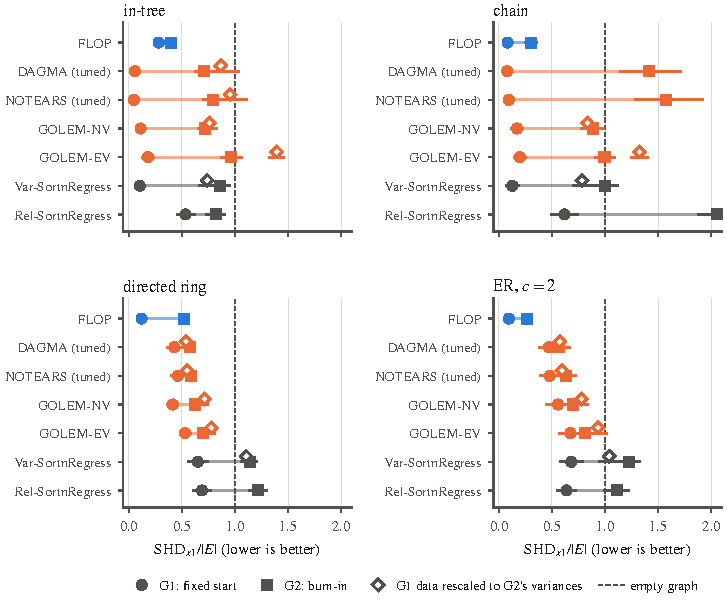
\includegraphics[width=\textwidth]{figs/fig_learners.pdf}
\caption{Learners under the fixed start (G1, circles) and a burn-in (G2, squares) on four summary-graph families
(SHD per true edge without first-slice edges; lower is better; 95\% graph-cluster intervals; dashed: the empty graph). On in-trees the
tuned continuous-optimisation methods (orange) beat FLOP (blue) under the fixed start and lose to it under the burn-in. Diamonds: the fixed-start data rescaled to the
marginal variances of the burn-in, which removes the advantage and over-corrects (see text). The panels use only the cells every method has
($p,T\in\{(5,3),(5,5),(10,3)\}$, see \texttt{figs/fig\_learners.py}); the tables pool each method over its own cells.}
\label{fig:learners}
\end{figure}

\begin{table}[t]
\caption{Scoring without the edges that leave the first slice (post hoc
re-analysis of committed B1 and learner-extension data; no new data). Gains
are G1$-$G2 in order accuracy; shifts are G2$-$G1 in SHD$/|E|$; the last three
rows (four methods) are the in-tree interactions of the rank change against FLOP (G1 value
minus G2 value of [method $-$ FLOP]). Graph-cluster 95\% CIs for the first
rows.}
\label{tab:x1}
\centering\small
\setlength{\tabcolsep}{3pt}
\begin{tabular}{@{}>{\raggedright\arraybackslash}p{0.44\textwidth}cc@{}}
\toprule
quantity & all edges & without slice-1 edges \\
\midrule
rel-SortnRegress, OA gain (300 non-SC graphs) & $+0.125$ [$0.116,0.134$] & $+0.089$ [$0.079,0.100$] \\
$R^2$-SortnRegress, OA gain & $+0.075$ & $+0.096$ \\
Var-SortnRegress, OA gain & $+0.210$ & $+0.195$ \\
FLOP, SHD$/|E|$ shift (420 graphs) & $+0.197$ [$0.185,0.209$] & $+0.093$ [$0.084,0.102$] \\
rel-SortnRegress, SHD$/|E|$ shift & $+0.649$ & $+0.531$ \\
in-tree interaction vs FLOP, DAGMA & $-0.524$ & $-0.587$ \\
\quad NOTEARS & $-0.369$ & $-0.462$ \\
\quad GOLEM-EV / GOLEM-NV & $-0.384$ / $-0.318$ & $-0.484$ / $-0.421$ \\
\bottomrule
\end{tabular}
\end{table}

\textbf{First-slice-excluded scoring.} Dropping the first-slice pairs removes
nearly a third of the rel-SortnRegress order-accuracy gain ($+0.125$ to
$+0.089$) and about half of FLOP's SHD shift ($+0.197$ to $+0.093$)
(\cref{tab:x1}); the artefact survives, and the rank changes against FLOP on
in-trees remain and grow slightly. For B1 and the learner extension the
full-window numbers stay the primary results of their own plans, and the
excluded-slice numbers are shown beside them.

\textbf{Further baselines.} On 384 new data sets (rings, chains, in-trees and
ER($c{=}2$); $p\in\{5,10\}$; $T\in\{3,5\}$) FLOP had the lowest mean SHD$_{x1}$
among the label-free methods (FLOP, GES from Tetrad, GRaSP and BOSS in
causal-learn, DirectLiNGAM, rel- and Var-SortnRegress) in 7 of 8 (family,
start) groups; the exception is in-trees under the fixed start, where
Var-SortnRegress ($0.136$) beat FLOP ($0.251$), which fits the variance
account. Mean SHD$_{x1}/|E|$ under the fixed start and after a burn-in was
$0.161$ and $0.353$ for FLOP, $0.358$ and $0.449$ for BOSS, $0.344$ and $0.522$
for GRaSP, $0.596$ and $0.944$ for GES, $1.417$ and $1.688$ for DirectLiNGAM,
$0.699$ and $1.392$ for rel-SortnRegress and $0.487$ and $1.139$ for
Var-SortnRegress; the empty graph scores $1$. Methods that use the time labels
are much closer to the truth and do not depend on the start: PCMCI+
\citep{runge2020pcmciplus} $0.021$ and $0.022$, DYNOTEARS \citep{pamfil2020dynotears}
$0.025$ and $0.047$, pooled lag-1 least squares $0.000$ and $0.071$, and a pooled
variant of VAR-LiNGAM \citep{hyvarinen2010varlingam} for replicated short
trajectories $0.007$ and $0.080$ (our noise is Gaussian, so its identifiability
condition does not hold). With the labels the gap to FLOP is $0.14$ under the
fixed start and $0.33$ after a burn-in. Every label-free method got worse under
the burn-in; PCMCI+ did not change.

\textbf{Takeaway (Q2, Q4).} The start changes what label-free learners appear
to do in two ways that the theory only partly covers. For the relatives sort,
the exact gap is the large-sample ceiling and the effect at a given sample size
is the detectable part of it. For tuned continuous-optimisation learners, a
fixed start produces a ranking change against FLOP on in-trees that variance
accounts for in part and that our theory does not predict.

\subsection{Real-data evidence: can relatives be estimated from one record?}
\label{sec:real}

\textbf{What this part tests.} The benchmark experiments give a method many
short replicate windows. A real record is one long, autocorrelated series, and
the question becomes whether the relatives of the unrolled structure can be
estimated from it at all (Q3), and whether the resulting count orients edges
(Q4). This differs from the effect of the start, and it is tested on few
independent units, because the units are segments of single records or
stations that recur across subgraphs (\cref{tab:units}). The overall result is
negative or does not discriminate between hypotheses.

\begin{table}[!ht]
\caption{What the inference of each study rests on. ``Units'' are the units
over which the reported intervals and p-values are computed.}
\label{tab:units}
\centering\small
\setlength{\tabcolsep}{3pt}
\begin{tabular}{>{\raggedright\arraybackslash}p{0.2\textwidth}>{\raggedright\arraybackslash}p{0.32\textwidth}>{\raggedright\arraybackslash}p{0.38\textwidth}}
\toprule
study & units used for inference & what is independent \\
\midrule
B1, B1-NL, learner extension (simulation) & summary graphs (cluster bootstrap) & graphs; each data set has $n=1000$ replicate trajectories of a short window \\
CausalRivers (P1--P6) & 120 subgraphs & 900 station slots, 445 distinct stations, one station used up to 7 times (112 of the 120 subgraphs share a station with another); two regions share a confounding driver; the 12\,h and 24\,h columns are the same records \\
wind tunnel (P7--P9) & 300 subgraphs, 15 runs & runs \\
E1 & 10 segments & one series (\texttt{citris\_1}) \\
B3 & 30 units & three runs of 30{,}000 steps \\
E2 & 64 held-out regimes, 1{,}280 subgraphs & regimes within runs; dependence between regimes not examined \\
\bottomrule
\end{tabular}
\end{table}

\begin{figure}[t]
\centering
\tikzfig{fig_units}
\caption{The units behind the inference of each study (\cref{tab:units}). Segments of one series, runs, and stations that recur across subgraphs are
not independent replicates, so the real-data results are effect sizes, not tests with nominal error rates.}
\label{fig:units}
\end{figure}

\textbf{Protocol and its limits.} We ran four studies (P1--P9, then E1/E2),
each with an analysis plan (predictions, thresholds, estimator, seeds, stop
conditions) committed to version control before any dependence statistic of its
data was computed (timeline in \cref{app:prereg}). Nine plans were written
in all, counting the plans of B1, B1-NL, B3, the learner extension and the
controls of \cref{sec:controls}, and the hosting service's push records were
retrieved for three of them. The
plans, analyses and
results were produced by AI agents within about six hours of one day, commit
times are set by the client and no external registry was used, so we call
them \emph{time-stamped analysis plans}, not pre-registrations. An earlier
exploratory project in the same repository had already found unrelated
CausalRivers stations about as correlated as river siblings, so our account of
that failure is explanatory, not predictive; and the graph refinement used by
E1 was motivated by study-3 observations on the same device
(\cref{app:prereg}).

\textbf{Estimand.} For an observed node set $O$ of a known summary graph, the
predicted value $\tilde s$ is the edge average of the scores of the counts
$|\rel_S(v)\cap O|$: population lag-0 relatives among the observed nodes, as a
perfect lag-0 dependence oracle would give them (\cref{prop:zero},
\cref{def:estimand}). $\tilde s>1/2$ forces an up-edge among the induced
edges, but not conversely (\cref{prop:estimand}, machine-checked). The
estimator is the relatives count of \cref{sec:finite} at $\alpha=0.01$ with
Bonferroni; orientation accuracy is the mean edge score of $\hat\rho$; CIs are
cluster bootstraps. \citet{lohse2025sortability} measured var- and
$R^2$-sortability on the same families; we know of no earlier test of
rel-sortability on real data.

\begin{sidewaystable}
\caption{Tests fixed in the time-stamped analysis plans. Pass/fail is by the point rule fixed in the plan.
Brackets: 95\% cluster-bootstrap CI. ``non-rel.\ dep.'': fraction of graph
non-relative pairs declared dependent. ``Acc.'': orientation accuracy on
edges predicted to be strictly sorted.}
\label{tab:real}
\centering
\setlength{\tabcolsep}{2.8pt}
\begin{tabular}{llll}
\toprule
study (units) & test (threshold) & result (12\,h / 24\,h) & verdict \\
\midrule
CausalRivers, marginal & P1: confluence subgraphs have $\tilde s>1/2$ & 112 of 114 & fails as worded$^a$ \\
(120 subgraphs) & P2: Acc.\ $>0.5$, CI excl.\ $0.5$ & $0.501\,[0.492,0.509]$ / $0.498\,[0.489,0.507]$ & \textbf{fail} \\
 & P3: Spearman$(\tilde s,\text{acc.})\ge0.3$ & $-0.018$ / $0.018$ & \textbf{fail} \\
 & \quad (non-rel.\ dep., nominal test) & $0.984$ / $0.978$ & stop condition met \\
\midrule
CausalRivers, conditioned & P4: non-rel.\ dep.\ $<0.5$ given proxy & $0.741$ / $0.735$ & \textbf{fail} \\
on regional proxy & P5: Acc.\ $>0.5$, CI excl.\ $0.5$ & $0.539\,[0.513,0.565]$ / $0.540\,[0.514,0.567]$ & pass, not interp.$^b$ \\
(120 subgraphs) & P6: Spearman $\ge0.3$ & $-0.113$ / $-0.121$ & \textbf{fail} \\
\midrule
Causal Chambers, wind & P7: non-rel.\ dep.\ $<0.5$ & $0.039\,[0.031,0.047]$ & pass \\
tunnel (15 runs, primary) & P8: Acc.\ $>0.5$, CI excl.\ $0.5$ & $0.656\,[0.637,0.675]$ & pass \\
 & P9: Spearman $\ge0.3$ (300 subgraphs) & $0.267\,[0.163,0.368]$ & \textbf{fail} \\
\midrule
light tunnel (10 segments, & R7 / R8 / R9 (same thresholds) & $0.000$ / $1.000$ / $0.779\,[0.696,0.864]$ & pass (replication)$^c$ \\
replication) &&& \\
\midrule
E1, light tunnel & E1a: non-rel.\ dep.\ $<0.5$; det.\ $\ge0.8$ & $0.000$; $0.969\,[0.945,0.992]$ & pass \\
(10 units, $G_{\mathrm{lin}}$) & E1b: $\Delta\le-0.10$, Holm $p\le0.05$, all 8 & $\Delta=-0.502$ to $-0.533$ (10/10) & pass (8/8)$^d$ \\
 & E1c: as E1b, detected edges & $\Delta=-0.500$ & pass (8/8) \\
\midrule
E2, wind regimes & Q7: non-rel.\ dep.\ $<0.5$ & $0.003\,[0.001,0.005]$ & pass \\
(64 units; $D{=}1$, & Q8: Acc.\ $>0.5$, CI excl.\ $0.5$ & $0.553\,[0.527,0.579]$ & pass \\
lags $L{=}30$ vs.\ 0) & Q9: Spearman $\ge0.3$ (1,280 subgr.) & $0.243\,[0.193,0.294]$ & \textbf{fail} \\
 & Q10: detection gain, CI lower bound $>0$ & $+0.069\,[0.060,0.079]$ & pass \\
 & E2 success (Q7--Q10 all) & & \textbf{not met} \\
\bottomrule
\end{tabular}
\par\smallskip 
{\footnotesize $^a$The two exceptions are split-and-rejoin channels with a
single source, for which the theorem itself predicts $1/2$.
$^b$Stop condition (P4 failed at both resolutions): P5 is reported, not
interpreted. $^c$Fixed in the plan as not counting towards a positive
demonstration (i.i.d.\ inputs, weak time-series aspect).
$^d$$G_{\mathrm{lin}}$ is the primary graph fixed in plan 4. It omits six real causal edges
that, under a symmetry lemma and an assumption of ideal polariser sensors, carry no linear dependence.
On the published graph the theorem still beats all eight overall, but not on its strictly
ordered edges, and on $G_{\mathrm{lin}}$ the prediction equals a weak-component-size rule (\cref{sec:real}, \cref{app:e1}).}
\end{sidewaystable}
\textbf{CausalRivers: a failed test, explained post hoc.} River networks
are in-forests, so \cref{cor:statiff} predicts $\tilde s>1/2$ for subgraphs
with confluences (mean $0.82$). The estimated relatives sort carried no
orientation information (P2, P3 fail; \cref{tab:real}) because 98\% of
non-relative station pairs tested dependent. Read through F2 (post hoc),
non-relative correlations $\kappa\approx0.64$--$0.74$ give
$\nhalf\approx20$--$27$, while the records have $n=377$--$3{,}652$ steps, so the
study sat deep in the saturated regime (\cref{fig:sat}, \cref{app:real}),
where \cref{prop:f2} predicts $\hat s=1/2$; regional precipitation acts as a
latent driver. The F3 remedy fixed in plan 2 (conditioning on a leave-out
regional mean) also failed (P4: $0.74$), consistently with F3: the triad
estimate of the proxy's reliability, $\hat r\approx0.62$, is below the required
$r_{\mathrm{crit}}\approx0.87$, and the in-sample plug-in prediction of the
dependent fraction, $0.743$, matches the observed $0.741$. The 120 subgraphs
reuse stations (\cref{tab:units}), so subgraph-level intervals understate the
variance; wider intervals would leave P2 failed.

\textbf{Causal Chambers: designed independent sources.} In the wind-tunnel
random-walk runs \citep{gamella2025chambers} five actuators are independent
random walks, hence separate source SCCs, and 25 of 26 edges are predicted
strictly sorted. Saturation is absent (P7, $0.039$) and the relatives count
orients confluence edges above chance (P8, $0.656$), but the graded agreement
P9 missed its threshold ($0.267<0.3$), so by the plan the study is \emph{not}
a positive demonstration. The reason is F1: 16 of 26 edges are essentially
undetectable at lag~0 at $n\approx10^3$. The light-tunnel replication passes
all three criteria, and F-theory predictions from the first half of each unit
match the second half to within $0.02$ (\cref{tab:ftheory}, \cref{app:real}).
The wind-tunnel graph is bipartite, so the prediction coincides with
``sensors have more relatives than actuators''.

\textbf{E1 and B3: the theorem against naive rules.} Plan 4 tested the edge
values of \cref{cor:statiff} against eight naive predictors (sensor
indicator, ancestor count, in-degree, depth, ``every edge $1$'', \dots) on the
light-tunnel series \texttt{citris\_1} (10 units). On the primary graph
$G_{\mathrm{lin}}$ it passed 8/8 ($\Delta=-0.50$ to $-0.53$ in absolute loss,
10/10 units, Holm $p=0.0078$). This is weaker than it looks
(\cref{app:e1}): $G_{\mathrm{lin}}$ removes six real edges that carry no linear
dependence under an ideal-sensor assumption, and on the published graph the
sensor indicator wins on strictly predicted edges; each weak component of
$G_{\mathrm{lin}}$ has a single source, so the prediction coincides with the
rule ``tie iff same weak component, else compare component sizes''; and most
of the separation comes from ties. B3 (\cref{app:b3}) therefore used held-out
light-tunnel data whose components have several independent sources (30
units of three AR(1)-driven series; 20 units of an actuator collider), with
constant $1/2$ and the weak-component rule as competitors. On the 2{,}361
instances where the theorem and the weak-component rule disagree, the counts
were sorted as predicted in $99.8\%$ ($\Delta=-0.50$ against both tie rules,
30/30 units); in the collider, R$\to$G was sorted whenever B was observed
(264/264) and tied otherwise (123/123). On these instances the theorem
predicts strict order, so E1's naive sort rules agree with it there and are
separated only on the 1{,}251 predicted ties whose own edge is detected
($\Delta=-0.43$, 30/30 units). The test was low-risk (same device; colour edges
known to be detectable; results 3--4 minutes after the plan), and it failed
where the graph is unfaithful: with an almost constant source the tie rule won
($\Delta=+0.12$, 0/10 units), and in one series the data contradicted
$G_{\mathrm{lin}}$ (the design graph matched $0.96$ against $0.04$ where they
differ). The p-values of E1 and B3 rest on units that are not independent. The
ten E1 units are segments of one series, and a sign-flip test over ten units
cannot give a Holm-adjusted $p$ below $0.0078$ against eight competitors, which
is the value reported. The 30 B3 units come from three runs, and at the level of
runs a sign-flip test cannot give $p$ below $1/8$. We read E1 and B3 as
descriptions of effect sizes on one device, and not as tests with their nominal
error rates.

\textbf{E2: lagged relatives} (\cref{app:e2}). A Bonferroni max-over-lags
cross-correlation test \citep{haugh1976checking} on 64 held-out wind-tunnel
regimes raised detection from $0.328$ to $0.398$ without more false
positives, but failed the graded criterion ($0.243<0.3$), so E2 does not
succeed, and neither did the lag-0 estimator on these regimes.

\textbf{Run- and station-level inference.} A later plan (\cref{app:b1y})
recomputed the real-data evidence at the level of independent units from
committed results, with no new data. B3: the theorem sorted as predicted in 3
of 3 independent runs (H1) and 2 of 2 (H2), with 10 of 10 segments agreeing in
each run; with so few runs the smallest attainable one-sided sign-test $p$ is
$1/8$ and $1/4$, so no run-level test can reach $0.05$, and the segment-level
$p$-values above are not run-level evidence. CausalRivers: the analysed
subgraph set has 900 station slots and 445 distinct stations, one station is
reused up to 7 times, and 112 of its 120 subgraphs share a station with another
(25 connected components, the largest of 28 subgraphs); the 457 stations and
reuse of 8 quoted in earlier drafts belong to a different, earlier subgraph set
whose results are not analysed here. For the orientation accuracy of the
conditioned relatives sort (P5, 12\,h) a station bootstrap gives $0.539$
[$0.527,0.551$], but in random station-disjoint subsets of about 42 subgraphs
the lower bound of the interval exceeded $0.5$ in only $27\%$ of 200 orderings
(median lower bound $0.491$). The pass of P5 is therefore narrow and does not
hold in most station-disjoint subsets. Sensitivity of the plug-in test to its
truncation lag ($K\in\{20,50,100,300\}$): at most $4\%$ of decisions changed on
the primary wind-tunnel analysis and on the river data, and none of $2{,}730$ on
B3; the E1 levels analysis is less stable (up to $13\%$ changed). The
re-fetched data matched every recorded SHA-256 value, and the rebuilt river
caches were byte-identical. We conclude that the real-data tests cannot reach
conventional significance at the level of independent runs or stations, and we
read them as effect sizes.


\begin{figure}[t]
\centering
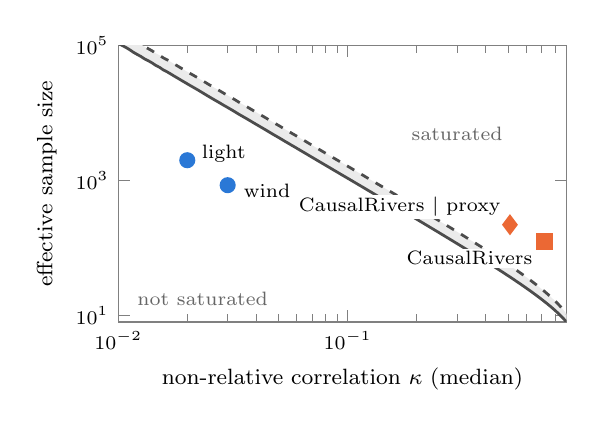
\begin{tikzpicture}
\begin{axis}[
  width=0.6\textwidth, height=0.42\textwidth,
  xmode=log, ymode=log, xmin=0.01, xmax=0.9, ymin=8, ymax=1e5,
  xlabel={non-relative correlation $\kappa$ (median)},
  ylabel={effective sample size},
  tick label style={font=\scriptsize}, label style={font=\footnotesize},
  axis line style={gray}, tick style={gray},
  legend style={font=\scriptsize, draw=none, fill=none, at={(0.98,0.98)}, anchor=north east},
  every axis plot/.append style={line width=1pt},
]
\addplot[name path=lo, domain=0.01:0.9, samples=120, black!70]
  {3 + (3.291/(0.5*ln((1+x)/(1-x))))^2};
\addplot[name path=hi, domain=0.01:0.9, samples=120, black!70, dashed]
  {3 + (4.044/(0.5*ln((1+x)/(1-x))))^2};
\addplot[black!8] fill between[of=hi and lo];
\addplot[only marks, mark=square*, mark size=2.6pt, color={rgb,255:red,235;green,104;blue,52},
  error bars/.cd, x dir=both, x explicit, y dir=both, y explicit]
  coordinates {(0.72,126) +- (0.02,13)};
\addplot[only marks, mark=diamond*, mark size=3pt, color={rgb,255:red,235;green,104;blue,52}]
  coordinates {(0.51,221)};
\addplot[only marks, mark=*, mark size=2.4pt, color={rgb,255:red,42;green,120;blue,214}]
  coordinates {(0.03,852) (0.02,1998)};
\node[font=\scriptsize, anchor=north east, fill=white, inner sep=1pt] at (axis cs:0.66,100) {CausalRivers};
\node[font=\scriptsize, anchor=south east, fill=white, inner sep=1pt] at (axis cs:0.48,260) {CausalRivers $\mid$ proxy};
\node[font=\scriptsize, anchor=west] at (axis cs:0.032,700) {wind};
\node[font=\scriptsize, anchor=west] at (axis cs:0.021,2500) {light};
\node[font=\scriptsize, black!60] at (axis cs:0.3,5e3) {saturated};
\node[font=\scriptsize, black!60, anchor=south west] at (axis cs:0.011,10) {not saturated};
\end{axis}
\end{tikzpicture}
\caption{Saturation regime of \cref{prop:f2}. Curves: onset $\nhalf$ for
$z_c=3.29$ ($d=5$, solid) and $4.04$ ($d=20$, dashed); above them a
non-relative pair is detected with probability $>1/2$. Points: medians from
the real-data studies (CausalRivers unconditioned and given the regional
proxy, $\kappa$ replaced by $|\pi|$; Causal Chambers wind and light tunnel).
Values are in \cref{tab:real} and \cref{app:real}.}
\label{fig:sat}
\end{figure}

\begin{table}[t]
\caption{Out-of-sample F-theory check on the Causal Chambers: predictions
from the first half of each unit, observed rates on the second half.
Accuracy is predicted by Monte Carlo of independent pair decisions.}
\label{tab:ftheory}
\centering
\setlength{\tabcolsep}{4pt}
\begin{tabular}{lcccc}
\toprule
 & \multicolumn{2}{c}{wind tunnel} & \multicolumn{2}{c}{light tunnel} \\
 & pred. & obs. & pred. & obs. \\
\midrule
non-relatives declared (F2) & 0.031 & 0.028 & 0.006 & 0.000 \\
relatives detected (F1) & 0.360 & 0.343 & 0.679 & 0.681 \\
orientation accuracy & 0.630 & 0.620 & 0.999 & 1.000 \\
\bottomrule
\end{tabular}
\end{table}

Data selection, preprocessing and secondary analyses are in \cref{app:real}.

\textbf{Takeaway (Q2, Q4).} Under a fixed start, the relatives-sorting
baseline does better in every simulated condition we tried. The controlled
tests of \cref{sec:controls} show that its gain follows the correlations a test
can detect, with the exact gap as the large-sample ceiling. Tuned competitive
learners change rank against FLOP on in-trees; variance is involved and does
not explain the effect alone. In real records the relatives count orients edges
only where the sources are designed to be independent and the relatives are
detectable, which was the case on one device. The real-data results are too
few, and too dependent, to say more.

%=============================================================================
\section{Discussion, Limitations and Conclusions}
\label{sec:disc}

\textbf{Question.} What should someone who builds a benchmark from an unrolled
graph do, and what do our results not show?

\subsection{Implications for benchmark design and real data}

\textbf{For benchmark design.} These recommendations apply when slices of a
simulated record are handed to a method that ignores time order; we found no
deployed generator that does so as shipped (\cref{sec:b1}). The finite
time-unrolled generator is rel-sortable above $1/2$ for every summary graph
that is not a union of strongly connected components (\cref{cor:iff}), strong
connectivity alone does not help at short horizons (\cref{sec:b1}), and part of
the excess comes only from the start at $t=1$. We recommend three things. (a)
Start trajectories from the stationary distribution (an exact
Lyapunov or Cholesky start, as in \citealp{herman2025unitless}), or use a
burn-in that is checked for distributional mixing. A burn-in of $\Delta$ slices
($\Delta\tau_{\max}$ with lags up to $\tau_{\max}$) removes the structural
artefact (\cref{thm:stat}); it is sufficient, it is the minimal burn-in
for chains (relatives: proved; value: computed for $p\le8$, $T\le5$) and for the
one-edge graph, and a shorter burn-in suffices for many
other graphs (\cref{rem:sharp}). It does not remove the distributional transient, which
decays with the spectral radius: B1 needed 100 steps to pass its mixing check.
As a rule of thumb, burn in for at least $\Delta$ slices and long enough for
the covariance to be near its stationary value, or draw the start from the
stationary law. (b) Report standardised
columns as well as raw ones, since the fixed start also inflates
var-sortability and the raw-data advantage of DAGMA and NOTEARS over FLOP under
the fixed start was reduced, and for DAGMA's SHD removed, on standardised data.
Standardisation alone is not a remedy: standardised DAGMA and GOLEM are below
chance in order accuracy. Tuning the hyper-parameters does not remove the effect
either: tuned DAGMA, NOTEARS and GOLEM-NV still beat FLOP on in-trees under the
fixed start (\cref{sec:controls}). (c) Score the window without first-slice pairs
or as an ADMG: a latent burn-in makes the last burn-in slice a set of latent
common causes of the first window slice, so a labels-using reference that has
normalised SHD $0.044$ under the fixed start has $0.273$ after a burn-in, but
$0.041$ against $0.048$ without first-slice pairs; dropping them reduced the
rel-SortnRegress gain from $+0.125$ to $+0.089$ and FLOP's SHD shift from
$+0.197$ to $+0.093$ (\cref{tab:x1}). An algorithm that sees time
stamps orients every cross-time edge for free, so the artefact matters for
methods that do not use time order. Random summary graphs are sortable only
near criticality. Removing the time labels does not hide the time order in
the population under the fixed start (\cref{sec:ident}), and for a method that
has the labels the start carries no extra information (\cref{prop:nogain}).

\textbf{For real data.} Population rel-sortability above $1/2$ does not imply
that a relatives count can be estimated. Two conditions are needed: no latent
common driver with share $\ell$ such that $n\gtrsim z_c^2/\ell^2$ (or a
near-perfect, rank-one proxy), and relatives detectable at lag~0 at the
available $\neff$. Diagnostic: compare $\neff$ with
$3+(z_c/\atanh\hat\kappa)^2$, where $\hat\kappa$ is the typical correlation of
pairs believed unrelated; if $\neff$ is far above it, the count is saturated
whatever the graph.

\subsection{Limitations}

The closed forms assume self-loops at every node and
unit lags (\cref{app:noloop,app:lags}). The burn-in bound is machine-checked sharp only
for one edge ($\Delta=1$), proved on paper to be sharp for the relatives of
chains, and not sharp in general; we have enumeration and no closed form for
the minimal burn-in. No human has compared the Lean statements with
the paper's statements. The spectral radii of the transition matrices of B1
were bounded by $0.8$ by construction and not tabulated. The ER limits are paper proofs not yet
checked by a human probabilist; they are iterated limits ($T\to\infty$ at
fixed $p$, then $p\to\infty$; the stationary value needs no $T$-limit), with
no rates and no result for fixed $T$. \Cref{sec:agg} covers linear SVARs only.
The finite-sample bounds are loose; \cref{prop:zero} and the probabilistic
parts of F1--F3 are proved on paper only, for Gaussian processes (the
non-Gaussian CLT step is cited, not re-proved), and our code's fixed $K$
controls size only away from a unit root. The analysis plans are internally
time-stamped and agent-executed (push order cannot show that nothing was
computed before a plan), and the CausalRivers plan was not blind to an
earlier analysis of the same data. The positive real-data evidence comes from
one device per chamber, and the units behind its p-values are not independent
(\cref{tab:units}); E1 coincides with a weak-component-size rule on its
primary graph and is carried mainly by ties; B3 separates the theorem from
that rule but on the same light tunnel, with no external registration. The
graded criteria P2, P3, P4, P6, P9, Q9 and one B3 secondary set failed. The
benchmark experiments are simulations at $n=1000$ (the dose study goes to
$25{,}000$ for three families); the learner extension uses one linear-Gaussian
parametrisation, $T\le5$ and default hyperparameters, and the tuned control
covers DAGMA, NOTEARS ($d\le30$) and GOLEM ($d\le50$) with $T\le10$ and
$p\le20$. Our theory does not predict the ranking changes among competitive
methods. They survive tuning and point to a variance channel by the plan's
rule, but imposing the fixed-start variances on burn-in data restored less than
half of the advantage, and we have no theory or experiment that explains the
rest; the plan's prediction of no rank change failed. The detectability calculation and the re-analyses with
graph-cluster inference are post hoc. The designed counterfactual separates the
population pattern from detectable correlations, but only for one estimator
(rel-SortnRegress) at $n=1000$ and in the dose study; we have not shown that the
exact gap itself, as opposed to its detectable image, drives the effect for any
learner. At the level of independent runs or stations the real-data tests
cannot reach conventional significance (B3 has three runs; the P5 interval
excludes $0.5$ in $27\%$ of station-disjoint subsets). Exposure of deployed generators to the variance
artefact was not measured (no mixing times). The identifiability statements
of \cref{sec:ident} are paper proofs that assume faithfulness, which we have
not shown to hold for almost all tied parameters; \cref{conj:window} is open;
and they give no finite-sample guarantee and no algorithm.

\subsection{Conclusions}

Time order survives label removal as a footprint that the unrolled graph
determines. For lag-one unrollings with self-loops we computed the footprint
exactly: the value of every edge, its limit, and a burn-in after which it no
longer depends on the start, with the graph statements checked in Lean. The
burn-in is sufficient, minimal for chains (proved for the relatives, computed for
the value with $p\le8$ and $T\le5$) and the one-edge graph, and longer than needed
for many other graphs. Under a fixed start the footprint is
inflated, strongly connected summary graphs are not protected at short
horizons, and a relatives-sorting baseline gained $0.13$ in order accuracy in
simulation. Controlled tests show that this gain follows the correlations a
test can detect, not the population relatives pattern, and that the exact gap is
the large-sample ceiling of the effect, reached in part ($0.76$) at
$n=25{,}000$. How much of the footprint an estimator sees depends on the sample
size, the autocorrelation and latent drivers; the real-data support was mostly
negative and, at the level of independent runs or stations, cannot reach
conventional significance. Tuned competitive learners change rank against FLOP
on in-trees under the fixed start; variance is involved but does not explain the
effect on its own, and our theory does not cover it. The finite-sample and
identifiability statements are paper proofs, with the limits listed above. A
builder who hands the slices of a simulated record to static learners should
start from the stationary distribution or use a burn-in that has been checked
for mixing, and should score the window without first-slice pairs.

\subsection{Use of AI tools}
\label{sec:aiuse}

Most of this project was carried out with AI coding agents (large language
models, Claude-based) working under the author's direction; no AI system is
an author. The paper proofs (including \cref{app:erproof,app:ident}), all Lean
code, all experiment and analysis code, the analysis plans, the simulated
pre-submission reviews that motivated several revisions, and the manuscript
text were generated by these agents. What is machine-checked: the Lean theorems
of \cref{sec:lean} (163 declarations in the axiom report, standard axioms only,
out of 259 theorem and lemma declarations in the sources), which cover the
exact and stationary results of \cref{sec:exact} including the $\Delta$ forms
of \cref{thm:limit,thm:stat} and the sharpness example for one edge, the
estimand algebra and the deterministic algebra of F1--F3. No human has
checked that the Lean statements say what the paper statements say; the map
in \cref{app:lean} is the agents' reading. What is checked only by
computation: the enumeration of \cref{app:enum,app:noloop}, the ER numerics
and the simulations of \cref{app:sims}. What no human has yet read line by
line: the paper-only proofs, namely \cref{app:erproof}, \cref{prop:zero},
\cref{thm:agg}, the probabilistic parts of
\cref{thm:f1,prop:nominal,prop:f2,prop:f3,prop:plugin}, \cref{prop:f1scope},
\cref{rem:nongauss}, the loop-free limit results of \cref{app:noloop}, the
lag-weighted extension (\cref{app:lags}), and
\cref{prop:nogain,prop:slices,prop:mec,prop:fixident,prop:nonident}. The
author takes responsibility for all content.

\backmatter

\bmhead{Supplementary information}
Code, a pinned environment (\texttt{requirements.txt}; Lean 4.35.0, Mathlib
v4.35.0), dataset sources with SHA-256 checksums (\texttt{DATA.md}), the
analysis plans, run logs and a reproduction script (\texttt{reproduce.sh},
with stages for the Lean build, the graph checks, the simulations including
the benchmark experiments and the learner extension, the post hoc
re-analyses, and the real-data studies; \texttt{REPRODUCE.md}) accompany the
article. The full stages of the script have not been re-run end to end, because
of the CPU budget, and not every committed output can be regenerated by one
command: the seeds behind some random-graph tables were not recorded, the
sweeps of the C++ checks are not scripted, and the single random graph with
$p=10^6$ is not scripted (\texttt{REPRODUCE.md} lists them).

\section*{Statements and Declarations}

\begin{itemize}
\item \textbf{Funding.} The author received no funding for this work.
\item \textbf{Competing interests.} The author declares no competing interests.
\item \textbf{Ethics approval and consent to participate.} Not applicable.
The study uses simulations and public sensor data sets and involves no human
participants, human data or animals.
\item \textbf{Consent for publication.} Not applicable.
\item \textbf{Data availability.} No new data were collected. The real-data
studies use the public CausalRivers benchmark \citep{stein2025causalrivers} and
the public Causal Chambers data sets \citep{gamella2025chambers} (CC BY 4.0);
sources, versions and SHA-256 checksums are listed in \texttt{DATA.md} of the
supplementary repository, and the raw data are not redistributed. All
simulated data are regenerated from fixed seeds by the reproduction script.
\item \textbf{Code availability.} All code, including the Lean development, is
in the supplementary repository,
\url{https://github.com/vinhqdang/KAN_time_series} (directory \texttt{research/theory2}).
\item \textbf{Materials availability.} Not applicable.
\item \textbf{Author contributions.} Q.-V.~Dang is the sole author: he
conceived and directed the study, supervised the AI agents described in
\cref{sec:aiuse}, and takes responsibility for all content.
\item \textbf{Use of AI tools.} See \cref{sec:aiuse}.
\end{itemize}

\begin{appendices}
\crefalias{section}{appendix}
\crefalias{subsection}{appendix}
% Appendices of the journal version. Included from main.tex inside \begin{appendices}.

\section{Overview and status labels}
\label{app:overview}
\Cref{app:exact} gives full proofs of \cref{sec:exact} (including
\cref{rem:sharp}), \cref{app:enum} the exhaustive enumeration check,
\cref{app:aggstate,app:agg} the statements and proofs for \cref{sec:agg}, \cref{app:finite} the proofs of
\cref{sec:finite} (including the plug-in effective sample size and the scope
of the recovery bound), \cref{app:sims} the simulation checks of F1--F3,
\cref{app:lean} the map from statements to Lean names, \cref{app:real} data
selection and preprocessing for the real-data studies, \cref{app:estimand}
the real-data estimand $\tilde s$, \cref{app:prereg} the analysis-plan
timeline for all studies and experiments, prior exposure and deviations,
\cref{app:e1,app:e2} the experiments E1 and E2 in full,
\cref{app:noloop,app:lags,app:er,app:x3} the loop-free graphs, lagged
unrollings, the random summary graphs (with the full proof of \cref{prop:er}
in \cref{app:erproof}) and the accuracy interpretation,
\cref{app:b1,app:b1nl,app:b1x,app:b3} the benchmark experiment B1, its
replication B1-NL, the extension to competitive learners with the post hoc
re-analysis, detectability calculation and generator survey, and the
discriminating test B3, and \cref{app:ident} the proofs of
\cref{sec:labels,sec:ident}.

Status labels. \emph{Machine-checked}: a Lean theorem with no \texttt{sorry}
and only the standard axioms. \emph{Proved}: a complete paper proof given
here. \emph{Asymptotic}: a limit statement proved here from the multivariate
Breuer--Major theorem \citep{arcones1994limit,nourdin2011quantitative} (cited, not
re-proved). \emph{Sketched}: a derivation with one analytic step left out,
stated as such (used only for statements outside the main claims: the windowed
loop-free stationary value, the layered-DAG stationary value and the constants
of the lagged recovery bound).
\emph{Enumerated}: checked by exact computation on many instances, not proved.

%=============================================================================
\section{Proofs for Section~\ref{sec:exact}}
\label{app:exact}


\textbf{Definition of $\srho$, verbatim.} \citet[Sec.~2.2]{reisach2026topological}
(arXiv v1) write: ``For a graph $G=(V,E)$ with $|E|\ge1$ we define sortability
by the number of relatives, or rel-sortability for short, as
$s_\rho(G):=\frac{\sum_{(x,y)\in E}s_\rho(x,y)}{|E|}$ with
$s_\rho(x,y):=0$ if $\rho(x)>\rho(y)$, $\frac12$ if $\rho(x)=\rho(y)$, $1$ if
$\rho(x)<\rho(y)$, for $(x,y)\in E$.'' (their Eq.~(4); the cases are typeset as a
brace there), and add: ``Note that our definition differs from the sortabilities
in these works in that we count edges instead of paths.'' Our $\srho$ is this
edge average; in $\GT$ the edges are the copies $(i(t),j(t{+}1))$.

Throughout, $\GS=(V,\Es)$ has a self-loop at every node, $p=|V|\ge2$, and
$d(u,v)$ is as in \cref{sec:setting}. We use two facts of
\citet{reisach2026topological}, proved there for DAGs: (Thm.~1) if
$x\in\anc(y)$ then $\rel(x)\subseteq\rel(y)$; (Lemma~1, eq.~(10)) if
$x\in\anc(y)$ then $\rel(x)\subsetneq\rel(y)$ iff $\mathrm{roots}(y)\setminus
\mathrm{roots}(x)\ne\emptyset$, where $\mathrm{roots}(y)=\{x\in\anc(y):\anc(x)=\{x\}\}$.
Both are also machine-checked independently
(\lname{relSet_subset_of_edge}, and the direct characterisation
\lname{isRel_unrolled_iff}).

\begin{lemma}[ancestors in $\GT$]\label{lem:anc}
$u(s)\in\anc(v(t))$ iff $s\le t$ and $d(u,v)\le t-s$.
\lean{\lname{unrolled_reach_iff}, \lname{unrolled_reach_iff_dist}.}
\end{lemma}
\begin{proof}
Every edge of $\GT$ increases time by one, so a directed path from $u(s)$ to
$v(t)$ has $t-s$ edges, and its projection to $V$ is a walk of length $t-s$
from $u$ to $v$ in $\GS$ (self-loops allowed as steps). Such a walk exists iff
$d(u,v)\le t-s$: a walk contains a path, so its length is at least
$d(u,v)$; conversely, pad a shortest path with $t-s-d(u,v)$ self-loop steps at
$u$. Every such walk lifts to a directed path in $\GT$.
\end{proof}

\begin{lemma}[roots]\label{lem:roots}
$\mathrm{roots}(v(t))=\{u(1):d(u,v)\le t-1\}$, and
$\desc(u(1))=\{w(s):d(u,w)\le s-1\}$.
\lean{\lname{roots_unrolled_iff}, \lname{isRoot_unrolled_iff}, \lname{desc_root_unrolled_iff}.}
\end{lemma}
\begin{proof}
A node $u(s)$ with $s\ge2$ has the parent $u(s-1)$ through the self-loop, so
it is not a root; $u(1)$ has no parent. Apply \cref{lem:anc} with $s=1$, in
both directions.
\end{proof}

\begin{proof}[Proof of \cref{thm:edge}]
$i(t)$ is a parent of $j(t{+}1)$, so $\rel(i(t))\subseteq\rel(j(t{+}1))$ and
$\srho(e)\in\{1/2,1\}$, with value $1$ iff the inclusion is strict, iff
$\mathrm{roots}(j(t{+}1))\setminus\mathrm{roots}(i(t))\neq\emptyset$. By
\cref{lem:roots} this set is $\{u(1):d(u,j)\le t,\ d(u,i)>t-1\}$, and since
$d$ is integer-valued or $\infty$, $d(u,i)>t-1$ iff $d(u,i)\ge t$.
\end{proof}

\begin{proof}[Proof of \cref{prop:boundary} (and the general count)]
Since every ancestor of $y$ descends from a root of $y$ that is itself an
ancestor, $\rel(y)=\desc(\mathrm{roots}(y))$. By \cref{lem:roots},
$w(s)\in\rel(v(t))$ iff some $u$ has $d(u,v)\le t-1$ and $d(u,w)\le s-1$,
i.e.\ iff $s\ge1+m_t(v,w)$ with $m_t(v,w)=\min\{d(u,w):d(u,v)\le t-1\}$.
Counting $s\in\{1,\dots,T\}$ gives
$\rho(v(t))=\sum_{w}\max(T-m_t(v,w),0)$ (\lname{rho_unrolled_eq}). For
$t\ge p$ every finite $d(u,v)$ is at most $p-1\le t-1$, so the admissible $u$
are $\anc_S(v)$ and $m_t(v,w)=d(\anc_S(v),w)$, finite iff $w\in\rel_S(v)$ and
then at most $p-1<t\le T$. (The Lean statement \lname{rho_unrolled_large_t}
needs only $t\ge p$; an earlier hypothesis $T\ge p$ is redundant.)
\end{proof}

\begin{proof}[Proof of \cref{thm:limit}]
Crossing edge $(i,j)\in\Ex$: $j$ does not reach $i$, so $d(j,i)=\infty$, and
$u=j$ gives $d(j,j)=0\le t\le\infty$ for every $t$: all $T-1$ copies score
$1$. Edge in $\Eo$: $i$ and $j$ reach each other (or $i=j$), so for every $u$,
$d(u,i)<\infty$ iff $d(u,j)<\infty$. If the condition of \cref{thm:edge} held
with $d(u,i)=\infty$ then $d(u,j)=\infty>t$, a contradiction; hence it forces
$t\le d(u,i)\le\Delta$, and at most $N_T(i,j)\le\min(\Delta,T-1)$ copies score
$1$ ($\Delta\le p-1$, \lname{maxFinDist_le_card_sub_one}). Summing over the $(T-1)|\Es|$ edges,
\[
\srho(\GT)=\tfrac12+\frac{1}{2(T-1)|\Es|}\Big[(T-1)|\Ex|+\sum_{(i,j)\in\Eo}N_T(i,j)\Big],
\]
which gives both bounds; let $T\to\infty$. Lean: \lname{sRho_unrolled_bounds_maxFinDist}
(the $\Delta$ form), with the $p-1$ form \lname{sRho_unrolled_bounds} as a corollary.
\end{proof}

\begin{proof}[Proof of \cref{cor:iff}]
$\Ex=\emptyset$ iff no edge joins two SCCs. A weakly connected component made of
two or more SCCs is connected by undirected edges, one of which joins two
different SCCs; conversely a strongly connected component has no crossing
edge. The uniform bound is \cref{thm:limit} with $|\Ex|\ge1$. For the DAG case,
every SCC is a singleton, $\Ex$ consists of the $m$ non-loop edges, and
$|\Es|=m+p$.
\end{proof}

\begin{proof}[Proof of \cref{thm:stat}]
In $G_{B+T}$, by \cref{lem:roots} shifted by $B$, $w(s)\in\rel(v(t))$ iff some
$u$ has $d(u,v)\le t-1$ and $d(u,w)\le s-1$. For window nodes $t-1,s-1\ge
B\ge\Delta$, and every finite distance is at most $\Delta$, so the condition is
$u\in\anc_S(v)\cap\anc_S(w)$, independent of $s,t$. Hence
$\rel_W(v(t))=\{w(s)\in W: w\in\rel_S(v)\}$, of size $T|\rel_S(v)|$. On
$V\times\mathbb Z$, \cref{lem:anc} holds verbatim and the common ancestor can
be taken arbitrarily early, giving the same set. Each copy of $(i,j)$ therefore
compares $|\rel_S(i)|$ with $|\rel_S(j)|$; as $i\in\anc_S(j)$,
$\rel_S(i)\subseteq\rel_S(j)$, so the score is $1$ iff
$\rel_S(i)\ne\rel_S(j)$, and $1/2$ for self-loops.
Source SCCs: $\rel_S(j)\setminus\rel_S(i)\ne\emptyset$ iff
$\anc_S(j)\not\subseteq\rel_S(i)$ (if $z\in\rel_S(i)$ then
$\desc_S(z)\subseteq\rel_S(i)$). Every node of $\anc_S(j)$ is reached from some
$\sigma\in\Src(j)$, and $\desc_S(\sigma)\subseteq\rel_S(i)$ whenever
$\sigma\subseteq\rel_S(i)$. A source SCC meets $\rel_S(i)$ iff it reaches $i$
(its only ancestors are its own nodes), and then it is contained in
$\rel_S(i)$. So the condition is $\Src(j)\not\subseteq\Src(i)$, which, as
$\Src(i)\subseteq\Src(j)$, is $\Src(i)\ne\Src(j)$. Lean:
\lname{rhoBurn_eq_maxFinDist}, \lname{sBurn_eq_maxFinDist} (with $B\ge\Delta$), and the
$B\ge p-1$ forms \lname{rhoBurn_eq}, \lname{sBurn_eq} as corollaries.
\end{proof}

\begin{remark}[sharpness of $B\ge\Delta$ for one edge]\label{rem:sharp}
For the single edge $0\to1$ with self-loops, $\Delta=1$; with $B=1$ the window
value is the stationary value $1/2$, and with $B=\Delta-1=0$ it is at least
$2/3$ for every $T\ge2$ (\lname{edgeLoops_burn_sharp}). So $B\ge\Delta$ cannot be
lowered for this graph. This is all that is proved. Enumeration on 726 random
summary graphs gave the stationary value at $B=\Delta$ in all of them, and at
$B=\Delta-1$ in 281; in 445 it did not (\cref{app:b1}). Hence $\Delta-1$
suffices for some graphs, and the minimal sufficient burn-in of a given graph
can be shorter than $\Delta$. We have no proof that for every $\Delta\ge2$ some
graph needs exactly $\Delta$ slices, and no closed form for the minimal
burn-in. Proving the first, for instance for the directed chain with
self-loops, would turn the enumeration into a theorem.
\end{remark}

\begin{proof}[Proof of \cref{cor:statiff}]
If each weak component $C$ has a unique source SCC $\sigma_C$, then
$\Src(v)=\{\sigma_C\}$ on $C$ and $\Eu=\emptyset$. Conversely, if
$\Eu=\emptyset$, $\Src$ is constant along edges and hence on each weak
component; a node $v$ of a source SCC $\sigma$ has $\Src(v)=\{\sigma\}$, so
there is only one. Out-forests (at most one parent besides itself; acyclicity
is not needed, \lname{stat_half_of_outForest}) and strongly connected graphs
(\lname{stat_half_of_strong}) have one source SCC per component. In an
in-forest (acyclic apart from self-loops, out-degree at most one), if
$u\in\anc(v)$ then $\desc(u)$ is the unique downstream path through $v$, so
$\rel(v)=\anc(v)\cup\desc(v)$ (\lname{inForest_isRel_iff}); the source SCCs
are the headwaters, and $\Src(j)=\Src(i)\cup\bigcup_{k}\Src(k)$ over the other
parents $k$ of $j$, with disjoint headwater sets on different branches, so
$\Src(j)\ne\Src(i)$ iff $j$ is a confluence (\lname{inForest_up_iff}).
Out-degree at most one alone is not enough: for $a\rightleftarrows b$ with
$c\to a$, $a$ has two parents but the only source SCC is $\{c\}$.
\end{proof}

\begin{remark}[self-loops]
Without self-loops the lemmas fail: for the single edge $0\to1$ without loops,
$\srho(\GT)=1/2$ for every $T\ge2$ (\lname{edgeNoLoops_sRho}); with loops the
limit is $2/3$ (\lname{edgeLoops_limit}).
\end{remark}

%=============================================================================
\section{Exhaustive Enumeration Check}
\label{app:enum}

Before formalisation, every statement of \cref{sec:exact} was checked by
brute force (bitset relatives with the definitions of
\citealp{reisach2026topological}) on all $4+64+4096$ summary graphs with
$p=2,3,4$ (all $T\le9$) and on $10{,}000$ random graphs ($p=2$--$7$; Erd\H{o}s--R\'enyi,
DAG, in-forest, out-forest, chain with back edge and block-SCC families;
three values of $T\le14$ each, fixed seed). In total 46{,}724 (graph,~$T$)
cases and 1{,}895{,}609 edges were checked with zero failures of
\cref{thm:edge}, \cref{prop:boundary}, the bounds of \cref{thm:limit},
\cref{thm:stat} (with $B=p-1$ and $B=2p+1$) and the source-SCC
characterisation. The conjecture fixed in plan 1 (``an edge is strictly
sorted in the limit iff $|\rel_S(j)|>|\rel_S(i)|$'') disagreed with the exact
$\GT$ limit in 9{,}603 random graphs and never with the stationary value; the
conjecture is \cref{thm:stat}, not the limit of $\GT$.

%=============================================================================
%=============================================================================
\section{Block Means and Subsamples: Statements}
\label{app:aggstate}




For a stable linear SVAR with independent innovations, nodes with disjoint
summary ancestor sets are independent at all lags, and so are any per-node,
time-invariant transforms, including block means and subsamples; otherwise
the lag-0 covariance is nonzero for almost every parameter
(\cref{prop:zero}). So the population relatives of
contemporaneous values are $\rel_S$ for every observation scheme, and the
population relatives sort is the stationary value of \cref{thm:stat} (on
non-self-loop edges), not the finite-$\GT$ value. Var- and $R^2$-sortability
behave differently (\cref{thm:agg}): block means converge, at the textbook
Fej\'er rate for averages of a stationary series
\citep[Ch.~7]{brockwell1991time}, to the long-run structural model of
\citet{gong2017aggregated}, whereas subsamples keep the snapshot covariance. As a
consequence, for large block size, block-mean $R^2$-sortability is $0$ on
out-stars and $1$ on in-stars with at least two arms for all weights; on
out-stars subsampled data are $R^2$-sorted correctly on average ($0.84$) while
block means drift to $0$. We claim only these sortability consequences.


Assumptions: $X(t)=\sum_{\tau=1}^{L}A_\tau X(t-\tau)+\varepsilon(t)$, $t\in\mathbb Z$,
i.i.d.\ innovations with diagonal positive-definite covariance $\Sigma$, stable
(all roots of $\det(I-\sum_\tau A_\tau z^\tau)$ outside the unit disc),
stationary solution; the summary graph has $i\to j$ iff $(A_\tau)_{ji}\ne0$ for
some $\tau$. $\Gamma(h)$ is the autocovariance, $A(1)=\sum_\tau A_\tau$, and for a
block size $D$ the block means are $\bar Y_s=\frac1D\sum_{u<D}X(sD{+}u)$ and the
subsamples $Z_s=X(sD)$.

\begin{proposition}[relatives survive any per-node filter]\label{prop:zero}
If $\anc_S(i)\cap\anc_S(j)=\emptyset$ then $X_i$ and $X_j$ are independent at
all lags, and so are any per-node, time-invariant (possibly nonlinear)
transforms of them, including $\bar Y$ and $Z$ for every $D$. If the
ancestor sets intersect, $\Gamma(0)_{ij}$, $\mathrm{Cov}(\bar Y)_{ij}$ and the
long-run covariance are nonzero for Lebesgue-almost every parameter.
\nolean{needs the SVAR moving-average representation and real-analytic genericity}
\end{proposition}

\begin{theorem}[block means vs subsampling]\label{thm:agg}
(a) $\|D\,\mathrm{Cov}(\bar Y)-S_{LR}\|\le\frac1D\sum_h|h|\|\Gamma(h)\|$,
with $S_{LR}=(I-A(1))^{-1}\Sigma(I-A(1))^{-\top}$.
(b) If $\GS$ is acyclic apart from self-loops, $S_{LR}$ is the covariance of a
static SEM (this long-run SEM is due to \citealp[Eqs.~(5), (10)]{gong2017aggregated}) on $\GS$ with weights $A(1)_{ji}/(1-\lambda_j)$ and noise variances
$\sigma_j^2/(1-\lambda_j)^2$, $\lambda_j=A(1)_{jj}<1$.
(c) $\mathrm{Cov}(Z_s)=\Gamma(0)$ for every $D$.
(d) Hence, for large $D$, block-mean $R^2$-sortability is $0$ on out-stars and
$1$ on in-stars with $\ge2$ arms, for all weights; under subsampling every
contemporaneous criterion keeps its $\Gamma(0)$ value.
\lean{(a) counting identity \lname{fejer_identity}; (b) \lname{longrun_factor}, \lname{selfloop_sum_lt_one}; the probabilistic steps, the rate and (c)--(d) are not machine-checked.}
\end{theorem}
Part (a) is the standard Fej\'er/Ces\`aro computation for the variance of the
mean of a stationary series \citep[Ch.~7]{brockwell1991time}, written for
block means of a vector process; (b) is due to \citet{gong2017aggregated}; (c)
is stationarity. We claim only the sortability consequences (d).

The $R^2$ statement for stars strengthens the three-node analysis in
\citet[App.~D]{herman2025unitless}, whose qualitative message (that $R^2$
reflects connectivity, with an asymmetry between colliders and confounders)
we credit. Numerical observations (exact population moments, not proved):
mean block-mean $R^2$-sortability over 150 in-trees moves from $0.853$
($D=1$) to $0.834$ ($D=4$--$8$) and $0.880$ ($D=256$), so it is not monotone in
$D$; on out-stars subsampled data are $R^2$-sorted at $0.842$ on average while
block means give $0.546$ ($D=4$), $0.101$ ($D=16$) and $0$ in the limit.


\section{Proofs for the Block-Mean and Subsampling Statements}
\label{app:agg}

\begin{proof}[Proof of \cref{prop:zero}]
By the MA($\infty$) representation $X(t)=\sum_k\Psi_k\varepsilon(t-k)$, and
because $\Psi_k$ is supported on the reachability relation, $X_i(t)$ is a
measurable function of $\{\varepsilon_k(s):k\in\anc_S(i)\}$. Disjoint ancestor
sets mean independent innovation sets, so the processes $X_i$ and $X_j$ are
independent, and so are any per-node transforms. For the generic part, each
covariance entry is real-analytic in $(A,\Sigma)$ on the connected open set of
stable parameters with the given support, hence either identically zero or
nonzero almost everywhere. With all coefficients positive, including the
self-loop at a common ancestor $k$, all $\Psi$ entries are nonnegative and
$\Psi_{ik}(m),\Psi_{jk}(m)>0$ for all large $m$ (self-loops pad the walks), so
$\Gamma(0)_{ij}>0$; the same holds for $\Gamma(h)$, $h\ge0$, and therefore for
the Fej\'er sums and $S_{LR}$. ``Generic'' does not mean ``large'': with little
autocorrelation, $\Gamma(0)_{ij}$ along a lagged edge can be tiny (down to
$10^{-14}$ in our exact computations; exactly $0$ without autocorrelation).
\end{proof}

\begin{proof}[Proof of \cref{thm:agg}]
(a) $D^2\mathrm{Cov}(\bar Y)=\sum_{u,w<D}\Gamma(u-w)=D\Gamma(0)+\sum_{h=1}^{D-1}(D-h)(\Gamma(h)+\Gamma(-h))$
(the counting identity is \lname{fejer_identity}). The stable VAR has
$\|\Gamma(h)\|\le C r^{|h|}$, $r<1$, so $\sum_h|h|\|\Gamma(h)\|<\infty$ and
$S_{LR}=\sum_h\Gamma(h)=\Psi(1)\Sigma\Psi(1)^\top$ with
$\Psi(1)=(I-A(1))^{-1}$. Then
$S_{LR}-D\,\mathrm{Cov}(\bar Y)=\sum_{|h|\ge D}\Gamma(h)+\sum_{|h|<D}\frac{|h|}{D}\Gamma(h)$,
and $1\le|h|/D$ in the first sum.
(b) Write $I-A(1)=(I-\Lambda)-N$ with $\Lambda$ the diagonal and $N$ the
off-diagonal part; then $I-A(1)=(I-\Lambda)(I-\tilde B)$ with
$\tilde B=(I-\Lambda)^{-1}N$ strictly triangular in a topological order
(\lname{longrun_factor}, \lname{longrun_inv}). Under acyclicity the AR
polynomial factorises into univariate $\phi_j(z)=1-\sum_\tau(A_\tau)_{jj}z^\tau$;
stability, $\phi_j(0)=1$ and the intermediate value theorem give
$\phi_j(1)=1-\lambda_j>0$ (\lname{selfloop_sum_lt_one}).
(c) Stationarity.
(d) For a linear SEM $X=BX+e$ with noise variances $\omega$,
$R^2_i=1-1/(\Sigma_{ii}(\Sigma^{-1})_{ii})$ and
$(\Sigma^{-1})_{ii}=1/\omega_i+\sum_{k\in\mathrm{ch}(i)}B_{ki}^2/\omega_k$. In
an out-star with root $0$ and leaves $k$, $1-R^2_0=1/(1+\sum_kr_k)$ and
$1-R^2_k=1/(1+r_k)$ with $r_k=\omega_0B_{k0}^2/\omega_k>0$, so with $\ge2$
leaves the root has strictly larger $R^2$ than every leaf; the in-star is
symmetric. Strict inequalities in the limit SEM of (b), plus (a) and
continuity of $S\mapsto R^2$ at positive-definite $S$, give the claim for all
large $D$. Under subsampling every contemporaneous statistic is a function of
$\Gamma(0)$.
\end{proof}

%=============================================================================
\section{Proofs for Section~\ref{sec:finite}}
\label{app:finite}

Notation. $\hat C_{ab}=\frac1n\sum_t(X_a(t)-\bar X_a)(X_b(t)-\bar X_b)$,
$\hat r_{ab}=\hat C_{ab}/\sqrt{\hat C_{aa}\hat C_{bb}}$. Constants:
$B_{ab}$ as in the main text; $D_\gamma=\max_a2\sum_h\gamma_{aa}(h)^2$;
$\kappa_1=\max_a\sum_h|\gamma_{aa}(h)|$;
$\kappa_2=\max_{a\ne b}(\sum_h|\gamma_{aa}(h)|+\sum_h|\gamma_{ab}(h)|)$. For
i.i.d.\ sampling, $B_{ab}=1+\rho_{ab}^2$, $D_\gamma=2$, $\kappa_1=1$.

\begin{lemma}[Gaussian chaos tail]\label{lem:chaos}
Let $g\sim N(0,I_N)$, $A$ symmetric, $S=g^\top Ag-\mathrm{tr}A$. For $x>0$,
$P(S\ge2\|A\|_F\sqrt x+2\|A\|_{op}x)\le e^{-x}$, and the same for $-S$.
\lean{algebraic steps \lname{phi_le}, \lname{chernoff_logmgf_le}, \lname{chernoff_choice}, \lname{sqrt_two_v_x}; the probability statement is not machine-checked.}
\end{lemma}
\begin{proof}
Diagonalise; $S$ has the law of $\sum_i\lambda_i(g_i^2-1)$. For $2s\lambda<1$,
$\log Ee^{s\lambda(g^2-1)}=\varphi(s\lambda)$ with
$\varphi(u)=-\frac12\log(1-2u)-u=\sum_{k\ge2}(2u)^k/(2k)\le u^2/(1-2|u|)$ for
$|u|<1/2$. With $c=2\|A\|_{op}$, $v=2\|A\|_F^2$ and $0\le s<1/c$,
$\log Ee^{sS}\le vs^2/(2(1-cs))$. Markov's inequality with $t=\sqrt{2vx}+cx$,
$q=\sqrt{2x/v}$ and $s=q/(1+cq)$ gives exponent exactly $x$. This is the
Gaussian case of \citet[Prop.~1]{hsu2012tail}, who derive it from
\citet{laurent2000adaptive}; the proof here is self-contained.
\end{proof}

\begin{lemma}[exact variance]\label{lem:var}
With $\tilde\gamma_{ab}=\frac1n\sum_tX_a(t)X_b(t)=g^\top Ag$ for
$A=C^{1/2}MC^{1/2}$, $M=\frac1{2n}\begin{psmallmatrix}0&I\\I&0\end{psmallmatrix}$,
\[
2n\|A\|_F^2=\sum_{|h|<n}\Big(1-\tfrac{|h|}{n}\Big)\big[\gamma_{aa}(h)\gamma_{bb}(h)+\gamma_{ab}(h)\gamma_{ab}(-h)\big]\le B_{ab},
\]
$\|A\|_{op}\le\kappa_2/(2n)$; on the diagonal $2n\|A\|_F^2\le D_\gamma$ and
$\|A\|_{op}\le\kappa_1/n$; and $\bar X_a\sim N(0,\bar\sigma_a^2)$ with
$\bar\sigma_a^2\le\kappa_1/n$.
\lean{trace and Toeplitz algebra \lname{quad_M}, \lname{trace_MC}, \lname{lemma12_trace}, \lname{lemma12_fejer}, \lname{lemma12_le_B}, \lname{lemma12_diag_le_D}; the step $\|C^{1/2}MC^{1/2}\|_F^2=\mathrm{tr}(MCMC)$ and the operator-norm bounds are not machine-checked.}
\end{lemma}
\begin{proof}
$\|A\|_F^2=\mathrm{tr}(MCMC)$ and, with Toeplitz blocks
$(C_{ab})_{st}=\gamma_{ab}(s-t)$,
$4n^2\mathrm{tr}(MCMC)=2\sum_{s,t}[\gamma_{aa}(s-t)\gamma_{bb}(s-t)+\gamma_{ab}(s-t)\gamma_{ab}(t-s)]$
(using that $\gamma_{aa}$, $\gamma_{bb}$ are even); count pairs with $s-t=h$.
$\|A\|_{op}\le\|C\|_{op}\|M\|_{op}$ and $\|C\|_{op}$ is at most the largest
absolute row sum.
\end{proof}

\begin{lemma}[deviation event]\label{lem:dev}
Let $\varepsilon_{ab}=\sqrt{2B_{ab}x/n}+\kappa_2x/n+2\kappa_1y/n$ and
$\varepsilon_d=\sqrt{2D_\gamma y/n}+4\kappa_1y/n$. With probability at least
$1-d(d{-}1)e^{-x}-4de^{-y}$, $|\hat C_{ab}-\rho_{ab}|\le\varepsilon_{ab}$ for all
$a\ne b$ and $|\hat C_{aa}-1|\le\varepsilon_d$ for all $a$.
\lean{deterministic steps \lname{centred_cov_eq}, \lname{centred_dev_offdiag}, \lname{centred_dev_diag}, \lname{lemma13_eps}, \lname{lemma13_count}.}
\end{lemma}
\begin{proof}
$\hat C_{ab}=\tilde\gamma_{ab}-\bar X_a\bar X_b$. Apply \cref{lem:chaos,lem:var}
to each off-diagonal and diagonal $\tilde\gamma$, bound $|\bar X_a|\le
\sqrt{2\kappa_1y/n}$ by the Gaussian Chernoff bound, and take a union bound.
\end{proof}

\begin{lemma}[correlation perturbation]\label{lem:pert}
If $a',b'\in[1-\varepsilon_d,1+\varepsilon_d]$, $\varepsilon_d<1$ and
$|c'-\rho|\le\varepsilon$, then
$|c'/\sqrt{a'b'}-\rho|\le(\varepsilon+|\rho|\varepsilon_d)/(1-\varepsilon_d)$.
\lean{\lname{corr_perturb} (the hypothesis $|\rho|\le1$ of our earlier statement is not needed).}
\end{lemma}
\begin{proof}
$|c'/\sqrt{a'b'}-\rho|\le|c'-\rho|/\sqrt{a'b'}+|\rho||1/\sqrt{a'b'}-1|$, with
$1/\sqrt{a'b'}\le1/(1-\varepsilon_d)$ and $|1/\sqrt{a'b'}-1|\le\varepsilon_d/(1-\varepsilon_d)$.
\end{proof}

\begin{theorem}[recovery bound]\label{thm:f1}
For $x,y>0$ let $\varepsilon_{ab}$, $\varepsilon_d<1$ be as in \cref{lem:dev} and
$\delta_{ab}=(\varepsilon_{ab}+|\rho_{ab}|\varepsilon_d)/(1-\varepsilon_d)$. If
thresholds separate ($\delta_{ab}\le\tau_{ab}$ on non-relatives and
$|\rho_{ab}|-\delta_{ab}>\tau_{ab}$ on relatives), the declared set equals the true
one, and hence $\hat s=\srho^{\mathrm{pop}}$, with probability at least
$1-d(d{-}1)e^{-x}-4de^{-y}$. For a common threshold $\tau<\rho_{\min}$ the
failure probability decays as
$\exp(-n\min(\tau,\rho_{\min}-\tau)^2/(2(\sqrt B+\rho_{\max}\sqrt{D_\gamma})^2))$.
\lean{deterministic core \lname{thm15_det}, \lname{decide_eq_target}, \lname{corr_perturb}, \lname{sOf_cntDecl_congr}; Chernoff and trace algebra \lname{chernoff_choice}, \lname{phi_le}, \lname{lemma12_trace}, \lname{lemma12_le_B}. The Gaussian tail bound itself is not machine-checked.}
\end{theorem}
The proof combines a Gaussian-chaos tail bound (the Gaussian case of
\citealp[Prop.~1]{hsu2012tail}; see also \citealp{laurent2000adaptive}), an exact
finite-$n$ variance identity for $\hat r$, and a deterministic perturbation
lemma.

\begin{proof}[Proof of \cref{thm:f1}]
Set $\delta_{ab}=(\varepsilon_{ab}+|\rho_{ab}|\varepsilon_d)/(1-\varepsilon_d)$.
On the event of \cref{lem:dev}, \cref{lem:pert} gives
$|\hat r_{ab}-\rho_{ab}|\le\delta_{ab}$, so non-relatives satisfy
$|\hat r|\le\tau$ and relatives $|\hat r|>\tau$ (\lname{decide_eq_target},
\lname{thm15_det}). Equal declared sets give equal counts and hence
$\hat s=\srho^{\mathrm{pop}}$ (\lname{sOf_cntDecl_congr}). For a VAR observed
as a long stationary series, $\srho^{\mathrm{pop}}$ is the stationary value
of \cref{thm:stat} on non-self-loop edges (\cref{prop:zero}). Explicit form:
with $y=x+\log(4/(d-1))_+$ (\lname{explicit_y}) and a common threshold
$\tau<\rho_{\min}$,
$P(\hat R\ne R)\le2d(d{-}1)\exp\!\big(-n\min(\tau,\rho_{\min}-\tau)^2/(2(\sqrt B+\rho_{\max}\sqrt{D_\gamma})^2)(1+o(1))\big)$.
\end{proof}

\textbf{The multivariate Breuer--Major theorem.} We use it in the form stated
by \citet[Thm.~1.1]{nourdin2011quantitative}, who attribute the vector case to
\citet{arcones1994limit}: let $X=(X_k)_{k\in\mathbb Z}$ be a centred stationary
Gaussian process in $\mathbb R^d$ with covariances $r^{(i,l)}(j)=E[X^{(i)}_1X^{(l)}_{1+j}]$,
and $f:\mathbb R^d\to\mathbb R$ with $E f(X_1)^2<\infty$ and Hermite rank $q\ge1$
with respect to $X$ (orthogonal to all polynomials of degree $<q$, not to some of
degree $q$). If $\sum_{j\in\mathbb Z}|r^{(i,l)}(j)|^q<\infty$ for all $i,l$, then
$n^{-1/2}\sum_{k\le n}(f(X_k)-Ef(X_k))\Rightarrow N(0,\sigma^2)$ with
$\sigma^2=\mathrm{Var}f(X_1)+2\sum_{k\ge1}\mathrm{Cov}(f(X_1),f(X_{1+k}))\in[0,\infty)$.

\begin{proof}[Proof of \cref{prop:nominal}]
Take $d=2$, $X_k=(X_a(k),X_b(k))$ and, for $c\in\mathbb R^3$,
$f_c(x)=c_1(x_a^2-1)+c_2(x_b^2-1)+c_3(x_ax_b-\rho_{ab})$. $f_c$ is a centred
polynomial of degree $2$ without linear part, so it is orthogonal to every
polynomial of degree $\le1$ (odd Gaussian moments vanish); if it were orthogonal
to every polynomial of degree $2$ it would be orthogonal to itself, so either
$f_c(X_1)=0$ a.s.\ (then the partial sums vanish) or its Hermite rank is $2$.
The condition $\sum_h|\gamma_{ab}(h)|^2<\infty$ holds because the covariances are
absolutely summable and bounded. By the theorem and the Cram\'er--Wold device,
$\sqrt n(\tilde\gamma_{aa}-1,\tilde\gamma_{bb}-1,\tilde\gamma_{ab}-\rho_{ab})\Rightarrow N(0,V)$,
where, by Isserlis' theorem, $V(ab,cd)=\sum_h[\gamma_{ac}(h)\gamma_{bd}(h)+\gamma_{ad}(h)\gamma_{bc}(h)]$
(as in \cref{lem:var}). Centring by the sample means changes each entry by
$\bar X_a\bar X_b$, and $\sqrt n\bar X_a\bar X_b\to0$ in probability since
$E(\sqrt n\bar X_a)^2\le\kappa_1$ and $\bar X_b\to0$; Slutsky's lemma applies.
The delta method with gradient $(-\rho/2,-\rho/2,1)$ gives $\sqrt n(\hat r-\rho)
\Rightarrow N(0,W)$,
$W=V(ab,ab)-\rho[V(ab,aa)+V(ab,bb)]+\frac{\rho^2}{4}[V(aa,aa)+2V(aa,bb)+V(bb,bb)]$,
which equals $\sum_h\gamma_{aa}(h)\gamma_{bb}(h)$ for an independent pair (this is
$B_{ab}$ when all products $\gamma_{aa}(h)\gamma_{bb}(h)$ are nonnegative, and at most
$B_{ab}$ in general). Then $\sqrt{n}\,\atanh\hat r\Rightarrow N(0,W_{ab})$ under the
null and $P(|\atanh\hat r|>z_c/\sqrt{n-3})\to2\bar\Phi(z_c/\sqrt{W_{ab}})$, which
exceeds the nominal $\alpha/m$ in the limit whenever $W_{ab}>1$.
\end{proof}

\begin{lemma}[sample autocovariances]\label{lem:acvl2}
Let $X_a$ be a standardised stationary Gaussian series with $\sum_h|\gamma_{aa}(h)|\le\kappa_1$ and
$\hat\gamma_a(h)=\frac1n\sum_{t\le n-h}(X_a(t{+}h)-\bar X_a)(X_a(t)-\bar X_a)$. For $0\le h<n$,
$E(\hat\gamma_a(h)-\gamma_{aa}(h))^2\le(8\kappa_1+108\kappa_1^2)/n+2(h/n)^2\gamma_{aa}(h)^2$.
\end{lemma}
\begin{proof}
For $\tilde\gamma(h)=\frac1n\sum_{t\le n-h}X(t{+}h)X(t)$, $E\tilde\gamma(h)=(1-h/n)\gamma(h)$ and, by Isserlis,
$\mathrm{Var}\,\tilde\gamma(h)=n^{-2}\sum_{s,t\le n-h}[\gamma(s{-}t)^2+\gamma(s{-}t{+}h)\gamma(s{-}t{-}h)]\le2\kappa_1/n$,
since $|\gamma|\le1$ gives $\sum_k\gamma(k)^2\le\kappa_1$ and $\sum_k|\gamma(k{+}h)\gamma(k{-}h)|\le\kappa_1$. The
centring term is $-\bar X(S_1+S_2)/n+\frac{n-h}{n}\bar X^2$ with $S_1,S_2$ partial sums; $\bar X$, $S_1/n$, $S_2/n$ are
centred Gaussians with variance $\le\kappa_1/n$ and $E(UV)^2\le3\sigma^4$ for such pairs, so its second moment is
$\le27\kappa_1^2/n^2$. Combine with $(u+v+w)^2\le4u^2+4v^2+2w^2$ for $u+v$ and the bias $w=h\gamma(h)/n$.
\end{proof}

\begin{lemma}[plug-in Bartlett factor]\label{lem:plugin}
Let $X_a,X_b$ satisfy the assumptions of \cref{sec:finite} (no condition on their cross-dependence),
$\hat\rho_a(h)=\hat\gamma_a(h)/\hat\gamma_a(0)$, $\hat W_n=1+2\sum_{h=1}^{K_n}\hat\rho_a(h)\hat\rho_b(h)$ and
$W^\circ_{ab}=\sum_{h\in\mathbb Z}\rho_a(h)\rho_b(h)$. If $K_n\to\infty$ and $K_n/n\to0$, then
$|\hat W_n-W^\circ_{ab}|=O_P(n^{-1/2}+K_n/n)+2\sum_{h>K_n}|\rho_a(h)\rho_b(h)|\to0$; for fixed $K$,
$\hat W\to1+2\sum_{h\le K}\rho_a(h)\rho_b(h)$ in probability.
\end{lemma}
\begin{proof}
With $\Delta_a=\hat\rho_a-\rho_a$, on $\{\hat\gamma_a(0),\hat\gamma_b(0)\ge\frac12\}$ (probability $\to1$),
$|\Delta_a(h)|\le2|\hat\gamma_a(h)-\gamma_{aa}(h)|+2|\gamma_{aa}(h)||\hat\gamma_a(0)-1|$. Write
$\hat\rho_a\hat\rho_b-\rho_a\rho_b=\Delta_a\rho_b+\rho_a\Delta_b+\Delta_a\Delta_b$. By \cref{lem:acvl2},
$E\sum_{h\le K}|\hat\gamma_a(h)-\gamma_{aa}(h)||\rho_b(h)|\le\kappa_1\sqrt{c_0/n}+\sqrt2\kappa_1K/n$, so the linear terms
are $O_P(n^{-1/2}+K/n)$; by Cauchy--Schwarz and $E\sum_{h\le K}(\hat\gamma_a-\gamma_{aa})^2\le Kc_0/n+2\kappa_1(K/n)^2$,
$\sum_{h\le K}|\Delta_a\Delta_b|=O_P(K/n)$; the tail is at most $\sum_{h>K}|\rho_a(h)|\to0$.
\end{proof}
Only $K_n=o(n)$ is needed, because the target is a sum of products of two summable sequences; we do not rely on
general HAC bandwidth conditions.

\begin{proposition}[plug-in effective sample size]\label{prop:plugin}
Under the assumptions of \cref{prop:nominal}, use the plug-in threshold $\tanh(z_c/\sqrt{n/\hat B_{ab}-3})$ with
$\hat B_{ab}=\max(1,\hat W_n)$, where $1\le K_n=o(n)$.
(i) For an independent pair with $W_{ab}>0$ and $K_n\to\infty$, the false-positive probability tends to
$2\bar\Phi(z_c\sqrt{\max(1,W_{ab})/W_{ab}})$, which is $\alpha/m$ if $W_{ab}\ge1$ and smaller otherwise. For fixed $K$ it
tends to $2\bar\Phi(z_c\sqrt{\max(1,W^\circ_{K,ab})/W_{ab}})$, $W^\circ_{K,ab}=1+2\sum_{h\le K}\rho_a(h)\rho_b(h)$.
(ii) Every pair with $\rho_{ab}\ne0$ is declared with probability $\to1$.
(iii) If the non-relatives are independent pairs (summary non-relatives of a Gaussian VAR) and every relative has
$\rho_{ab}\ne0$, then $\liminf_nP(\hat R=R)\ge1-|N|\alpha/m\ge1-\alpha$, and the same holds for
$P(\hat s=\srho^{\mathrm{pop}})$, provided $K_n\to\infty$.
\nolean{uses the multivariate Breuer--Major theorem through \cref{prop:nominal}}
\end{proposition}
\begin{proof}
(i) $T=|\sqrt n\,\atanh\hat r|\,(1/\hat B-3/n)^{1/2}$. By \cref{prop:nominal}, $\sqrt n\,\atanh\hat r\Rightarrow N(0,W)$,
and $\hat B\to b=\max(1,W)$ (or $\max(1,W^\circ_K)$) in probability by \cref{lem:plugin}. By Slutsky,
$T\Rightarrow|N(0,W/b)|$, whose law has no atom at $z_c$. (ii) By \cref{lem:var}, $\hat r_{ab}\to\rho_{ab}$ in
probability. By Cauchy--Schwarz $|\hat\rho_a(h)|\le1$, so $\hat B\le1+2K_n=o(n)$ and $n/\hat B\to\infty$.
(iii) Union bound over $N$ with (i), and (ii) on $R$; equal declared sets give equal $\hat s$.
\end{proof}

\begin{proposition}[scope of \cref{thm:f1}]\label{prop:f1scope}
Let the non-relatives $N\neq\emptyset$ have deterministic thresholds with $n\tau_{n,ab}^2\to t_{ab}^2\in(0,\infty)$:
$t^2=z_c^2$ for the nominal Fisher-$z$ test, and $t^2=z_c^2b_{ab}$ for the effective one with $n'=n/b_{ab}$. Then the
smallest failure probability certified by \cref{thm:f1} tends to $d(d{-}1)\exp(-\min_Nt_{ab}^2/(2B_{ab}))>0$ when the
relatives have $|\rho|\ge\rho_{\min}>0$ (and is at least this in general). For i.i.d.\ data and the nominal test this
is $d(d{-}1)e^{-z_c^2/2}\ge\sqrt{2\pi}\,z_c\alpha$ (Mills), e.g.\ $0.089$ for $d=5$, $\alpha=0.01$. If instead
$\alpha_n\to0$ with $\log(1/\alpha_n)=o(n)$, \cref{thm:f1} gives
$P(\hat R\ne R)\le d(d{-}1)\exp(-(1-\eta)z_{c,n}^2r/2)+4d/n\to0$ for any $\eta>0$ and large $n$, with
$r=\min_N(n/n'_{ab})/B_{ab}$.
\end{proposition}
\begin{proof}
For $\rho_{ab}=0$ the separation condition $\delta_{ab}\le\tau_{n,ab}$ and $\varepsilon_{ab}\ge\sqrt{2B_{ab}x/n}$ force
$x\le n\tau_{n,ab}^2/(2B_{ab})$, which gives the lower bound. For attainment, take
$x_n=(1-\eta)\min_Nn\tau_{n,ab}^2/(2B_{ab})$ and $y_n=\log n$. Then all lower-order terms are $o(n^{-1/2})$ and
$\varepsilon_d\to0$, so the conditions hold for large $n$ on $N$, and on the relatives because $\tau_n\to0$. The
vanishing-level statement is the same computation with $z_{c,n}\to\infty$.
\end{proof}

\begin{remark}[non-Gaussian innovations]\label{rem:nongauss}
Let $X(t)=\sum_j\Psi_j\varepsilon(t-j)$ with $\sum_j\|\Psi_j\|<\infty$ and i.i.d.\ innovations with independent
unit-variance coordinates and fourth cumulants $\kappa_i=E\varepsilon_i^4-3$. Put
$G_i(a,b)=\sum_j\Psi_j[a,i]\Psi_j[b,i]$. Then $n\,\mathrm{Cov}(\tilde\gamma_{ab},\tilde\gamma_{cd})\to
V(ab,cd)+\sum_i\kappa_iG_i(a,b)G_i(c,d)$ (moment--cumulant formula and dominated convergence), so
$W_{ab}^{\mathrm{ng}}=W_{ab}+\sum_i\kappa_ig_i^2$ with $g_i=G_i(a,b)-\frac{\rho_{ab}}2(G_i(a,a)+G_i(b,b))$. Independent
series share no innovation, so $g_i=0$: the null variance $\sum_h\rho_a(h)\rho_b(h)$, and hence
\cref{prop:nominal,prop:plugin}, are unchanged, given the CLT for linear processes, which we do not re-prove. For
relatives, $W$ changes by $\sum_i\kappa_ig_i^2$ (of either sign, since $\kappa_i\ge-2$). This affects power and
transition widths, not the population statements or the location of $\nhalf$. The non-asymptotic bounds use the
Gaussian chaos tail. For sub-Gaussian innovations the Hanson--Wright inequality
\citep[Thm.~1.1]{rudelson2013hanson} has the same form with unspecified constants.
\end{remark}

\textbf{Fixed $K$ in practice (simulation and data check).} Independent AR(1)
pairs, 4{,}000 replications (2{,}000 at $n=64{,}000$): at AR coefficient
$0.9$ and $0.97$ the plug-in test with $K=50$ has size $0.050$ and $0.056$
(level $0.05$; limits $0.05$ and $0.0556$), but at $0.99$ it has $0.113$
(limit $0.118$), while $K_n=n^{0.6}$ gives $0.0495$ and the nominal test
$0.853$; for the opposite-sign pair the floor makes the test conservative
(size $0$). On the B3 primary data (30 segments of 3{,}000 rows, 2{,}730
unit-pairs) the declared status of no pair changes when $K=50$ is replaced
by $55$, $122$ or $300$ (post hoc). This was not checked for study 3, E1 or
the river data. Scripts: \texttt{finite2/}.


\textbf{F2 and F3.} The statements are \cref{prop:f2,prop:f3} in \cref{sec:finite}.

\begin{proof}[Proof of \cref{prop:f2}]
$\mathrm{Cov}(X_u,X_v)=\gamma^Y_{uv}(0)+b_ub_v$ and $\gamma^Y_{uv}=0$ for
non-relatives (\cref{prop:zero}); divide by the standard deviations
(\lname{prop21_corr_std}). For relatives the sum is nonzero except on a
Lebesgue-null set. All counts equal $d$, so every edge scores $1/2$
(\lname{sOf_saturated}). The rate: apply \cref{thm:f1} with target ``all
pairs'' and $x=y=cn$, $c$ small enough that $\delta\le\kappa_{\min}/3$ and
$\tau_n\le\kappa_{\min}/3$ eventually; $|\hat s-1/2|\le1/2$ always
(\lname{abs_sOf_sub_half_le}). The onset: by the asymptotic normality of
$\atanh\hat r$, the declaration probability crosses $1/2$ where
$\tanh(z_c/\sqrt{n-3})=|\kappa|$, i.e.\ at $\nhalf$ (\lname{ncrit_eq_iff}).
\end{proof}


\begin{proof}[Proof of \cref{prop:f3}]
$\mathrm{Cov}(X_u,Z)=b_u\sqrt r$ and $\mathrm{Var}Z=1$; the partial covariance
is $\gamma^Y_{uv}+(1-r)b_ub_v$ and the partial variance
$\mathrm{Var}Y_u+(1-r)b_u^2$; divide and standardise (\lname{prop31},
\lname{prop31_std}; positive $\mathrm{Var}Y_u$ is required). At $r=1$,
$\pi=\rho^Y$ (\lname{cor32}). For non-relatives
$|\pi_{uv}|=\sqrt{\ell_u\ell_v}\sqrt{f_uf_v}$ with $f_w(r)=(1-r)/(1-r\ell_w)$
and $f_w'(r)=(\ell_w-1)/(1-r\ell_w)^2<0$ (\lname{absPi_strictAntiOn},
\lname{absPi_eq_zero_iff}; both need $b_ub_v\ne0$). Bounds
$(1-r)\sqrt{\ell_u\ell_v}\le|\pi|\le(1-r)\sqrt{\ell_u\ell_v}/(1-\ell_{\max})$
(\lname{absPi_lower}, \lname{absPi_upper}). $r_{\mathrm{crit}}$ solves
$(1-r)\ell/(1-r\ell)=\tau'$ (\lname{rcrit_iff}, \lname{rcrit_example}). The
finite-sample bracket uses the Lipschitz bound
$|g(a',b',c')-g(a,b,c)|\le L(q)\max(|a'-a|,|b'-b|,|c'-c|)$ for
$g(a,b,c)=(a-bc)/\sqrt{(1-b^2)(1-c^2)}$, $|b|,|c|\le q<1$,
$L(q)=1/(1-q^2)+4q/(1-q^2)^2$ (\lname{pc_lipschitz}, \lname{thm35_bracket}),
combined with \cref{lem:dev} for $(X,Z)$. Multi-filter driver: for
$D_v(t)=b_vC(t-k_v)$ with $C$ an AR(1) with coefficient $\phi$ and $Z=C(t)$,
\[
\pi_{uv}=\frac{b_ub_v(\phi^{|k_u-k_v|}-\phi^{k_u+k_v})}{\sqrt{(s_u^2-b_u^2\phi^{2k_u})(s_v^2-b_v^2\phi^{2k_v})}},
\]
nonzero for $k_u,k_v>0$, $\phi\in(0,1)$, $b_ub_v\ne0$ (\lname{prop36_ar1},
\lname{prop36_ar1_ne_zero}); in general $\pi_{uv}\propto\mathrm{Cov}(D_u-P_ZD_u,D_v-P_ZD_v)$
vanishes for all non-relative pairs iff the residual driver components are
uncorrelated, which holds for a rank-one driver with $Z=F$
(\lname{prop36_pcov}, \lname{prop36_zero_iff}, \lname{prop36_rank_one}). A
proxy that contains summary relatives of $u,v$ adds the terms
$-c_Z(b_uq_v+b_vq_u)-q_uq_v$ to the numerator (\lname{prop37_pcov},
\lname{prop37_bound}). Triad identity: $\rho_{uZ}\rho_{vZ}/\rho_{uv}=r$ and, for
$r>0$, $\ell_u=\rho_{uZ}^2/r$ (\lname{prop38_ratio}, \lname{prop38_loading}).
\end{proof}

%=============================================================================
\section{Simulation Checks of F1--F3}
\label{app:sims}

All with fixed seeds; full tables are in the supplementary material.
\textbf{F1} (5 processes: in-forests with $d=5$ and $d=10$, self-loop
persistence $\lambda\in\{0.5,0.9,0.97\}$, and a near-white-noise case;
$n=200$--$20{,}000$; 1{,}000 replications per cell; nominal, oracle-effective
and fixed thresholds). The bound was never violated in 105 cells. It is loose:
with a fixed threshold $\rho_{\min}/2$, it reaches $0.9$ at about 3--13 times
the $n$ at which the simulated probability does, and much later with
Bonferroni thresholds, where the Chernoff step loses the Mills-ratio factor.
The empirical $n\,\mathrm{Var}(\hat r)/W$ lies in $[0.93,1.11]$. With the
nominal test, $P(\hat R=R)$ plateaus at $0.94$, $0.22$, $0.03$ and $0.27$, as
\cref{prop:nominal} predicts (predicted vs simulated false-positive rates,
e.g.\ $0.33$ vs $0.32$--$0.33$ at $\lambda=0.9$).
\textbf{F2} ($\ell\in\{0.02,0.1,0.3,0.64\}$): the asymptotic detection curve
matches the simulated fraction of declared non-relatives within $0.02$ for
$n\ge200$; predicted $\nhalf=1{,}079$ for $\ell=0.1$, simulated $0.479$ at
$n=1{,}000$.
\textbf{F3}: predicted $n_{\mathrm{crit}}=472$ ($\ell=0.64$, $r=0.9$) gives a
simulated declared fraction $0.495$ at $n=471$; over 38 cells the asymptotic
prediction is within $0.03$. With travel-time lags $(0,1,2,4,8)$, $\phi=0.9$,
$r=1$, the declared fraction still rises to $0.63$ at $n=10{,}000$, as the
multi-filter part of \cref{prop:f3} predicts.

%=============================================================================
\section{Lean Formalisation: Map and Findings}
\label{app:lean}

Lean 4.35.0 and Mathlib v4.35.0; 4{,}159 lines in 16 files. The build log
(a clean rebuild of the final state, 9{,}064 jobs, including \lname{Observed.lean}
and the $\Delta$ refinements),
the \texttt{\#print axioms} output for each of the 163 declarations in the axiom
report (all \texttt{[propext, Classical.choice, Quot.sound]}) and a grep showing
no \texttt{sorry}/\texttt{admit}/\texttt{axiom} are in the supplementary
material.

\textbf{What is and is not certified.} Certified: the exact and stationary
results of \cref{sec:exact}, the loop-free exact edge value, the accuracy
reading, the algebra of the estimand $\tilde s$ (\cref{app:estimand}), and the
deterministic and algebraic parts of \cref{sec:agg,sec:finite}. Not certified:
the ER limits (only the deterministic witness lemmas), the loop-free limit,
periodicity and stationary value, the lag-weighted extension, and every
probability bound, limit theorem and genericity statement.

\textbf{Breakdown of the 163 declarations} (counted from the Lean files):
33 headline theorems, i.e.\ Lean counterparts of numbered paper statements
(29 for \cref{sec:exact}, the loop-free edge value and the accuracy reading,
including the four $\Delta$ forms of \cref{thm:limit,thm:stat,cor:statiff}; 4
for \cref{prop:estimand}); 53 supporting graph lemmas (ancestry, roots, distance,
the largest finite distance $\Delta$ (\lname{maxFinDist}, 10 lemmas), source SCCs,
5 ER witness lemmas, 6 estimand lemmas); 65 algebraic identities
and inequalities of the aggregation and finite-sample files (correlation
perturbation, Chernoff algebra, trace and Toeplitz identities, partial
correlation formulas, threshold locations; several are elementary, e.g.\
$|\hat s-\tfrac12|\le\tfrac12$); 12 examples (10 concrete graphs, the sharpness
example \lname{edgeLoops_burn_sharp}, 1 numerical $r_{\mathrm{crit}}$ instance).
The sources contain 259 theorem and lemma declarations in all; the axiom
report lists the 163 above, and the other 97 are not in it. No human has
checked, line by line, that each Lean statement says what the corresponding
paper statement says; the map below is the authors' (AI-generated) reading.

\begin{center}\small
\begin{tabular}{>{\raggedright\arraybackslash}p{0.21\textwidth}>{\raggedright\arraybackslash}p{0.53\textwidth}>{\raggedright\arraybackslash}p{0.16\textwidth}}
\toprule
statement & Lean names & status \\
\midrule
\cref{lem:anc,lem:roots} & \lname{unrolled_reach_iff}, \lname{unrolled_reach_iff_dist}, \lname{roots_unrolled_iff}, \lname{desc_root_unrolled_iff}, \lname{isRel_unrolled_iff} & checked \\
\cref{thm:edge} & \lname{edge_score}, \lname{edge_score_dist}, \lname{strictCond_iff_dist} & checked \\
\cref{prop:boundary} & \lname{rho_unrolled_eq}, \lname{mT_le_iff}, \lname{rho_unrolled_large_t} & checked \\
\cref{thm:limit} & \lname{sRho_unrolled_exact}, \lname{sRho_unrolled_bounds_maxFinDist} ($\Delta$ form), \lname{sRho_unrolled_bounds} ($p-1$ form), \lname{tendsto_sRho_unrolled}, \lname{tendsto_sRho_GT}; $\Delta$: \lname{maxFinDist}, \lname{dist_le_maxFinDist}, \lname{exists_dist_eq_maxFinDist}, \lname{maxFinDist_le_card_sub_one} & checked \\
\cref{cor:iff} & \lname{tendsto_half_iff}, \lname{crossEdges_eq_empty_tfae}, \lname{sRho_unrolled_ge_of_cross}, \lname{reisach_theorem4}, \lname{limitValue_dag} & checked \\
\cref{thm:stat} & \lname{rhoBurn_eq_maxFinDist}, \lname{sBurn_eq_maxFinDist}, \lname{relBurn_iff_maxFinDist}, \lname{walkN_of_reach_maxFinDist} ($B\ge\Delta$); \lname{rhoBurn_eq}, \lname{sBurn_eq} ($B\ge p-1$); \lname{rhoZ_eq}, \lname{sZ_eq}, \lname{sOf_window}, \lname{relSet_eq_iff_src}, \lname{mem_upEdges_iff} & checked \\
\cref{rem:sharp} (sharpness of $B\ge\Delta$ for one edge) & \lname{edgeLoops_burn_sharp}, \lname{sBurn_zero}, \lname{relBurn_zero_iff}, \lname{maxFinDist_edgeLoops} & checked \\
\cref{cor:statiff} & \lname{sBurn_eq_half_iff_maxFinDist}, \lname{sBurn_eq_half_iff}, \lname{sBurn_eq_half_iff_common_anc}, \lname{sZ_eq_half_iff}, \lname{upEdges_eq_empty_tfae}, \lname{stat_half_of_strong}, \lname{stat_half_of_outForest}, \lname{inForest_isRel_iff}, \lname{inForest_up_iff}, \lname{statValue_inForest}, \lname{statValue_inForest_gt_iff} & checked \\
\cref{tab:examples} & \lname{collider_limit}, \lname{fork_limit}, \lname{chain3_limit}, \lname{collider_stat}, \lname{fork_stat}, \lname{chain3_stat} & checked \\
self-loop remark & \lname{edgeLoops_limit}, \lname{edgeNoLoops_sRho} & checked \\
\cref{thm:noloop} (ancestors, relatives, edge value) & \lname{isRel_unrolled_iff_NL}, \lname{reduce_ancestor}, \lname{relSet_unrolled_eq_iff_NL}, \lname{edge_score_NL} & checked \\
\cref{cor:noloop} & \lname{sRho_unrolled_eq_NL}, \lname{sRho_unrolled_ge_half_NL} & checked \\
\cref{prop:noloopcross} (witness $u=j$, fresh parent) & \lname{strictNL_of_closed_walk}, \lname{strictNL_of_fresh_parent}, \lname{sRho_unrolled_eq_one_NL} & checked \\
loop-free examples (\cref{tab:noloop}) & \lname{colliderNL_sRho}, \lname{edgeLoopHead_sRho}, \lname{edgeNoLoops_sRho} & checked \\
eventual periodicity, limit, same-SCC edges, \cref{thm:noloopstat} & -- & paper / enumerated \\
\bottomrule
\end{tabular}
\end{center}

\begin{center}\small
\begin{tabular}{>{\raggedright\arraybackslash}p{0.21\textwidth}>{\raggedright\arraybackslash}p{0.53\textwidth}>{\raggedright\arraybackslash}p{0.16\textwidth}}
\toprule
statement & Lean names & status \\
\midrule
\cref{prop:er} & witness lemmas \lname{upEdge_witness}, \lname{mem_upEdges_of_witness}, \lname{mem_upEdges_of_disjoint_anc}, \lname{upEdges_subset_confluenceNL}, \lname{card_upEdges_le_confluenceNL} & paper proof (App.~\ref{app:erproof}); lemmas checked \\
\cref{prop:lags} & -- & paper only \\
\cref{prop:estimand} (a)--(d) & \lname{relObs_subset_of_edge}, \lname{score_obsEdge}, \lname{sTilde_eq}, \lname{sTilde_ge_half}, \lname{upObs_subset_upEdges}, \lname{sTilde_gt_half_iff}, \lname{exists_upEdge_of_sTilde_gt_half}, \lname{sTilde_eq_half_of_no_up}, \lname{mem_upObs_of_witness}, \lname{upObs_univ} & checked \\
\cref{prop:x3} (oracle sort accuracy; optimality) & \lname{accRule_sortRule}, \lname{accRule_sortRule_rho}, \lname{accRule_le_sOf}, \lname{accRule_le_sRho}, \lname{edgeAcc_sortRule_strict}, \lname{rho_not_gt_of_edge} & checked \\
\cref{prop:zero} & -- & paper only \\
\cref{thm:agg}(a) & \lname{fejer_identity} (counting identity) & partial \\
\cref{thm:agg}(b) & \lname{longrun_factor}, \lname{longrun_inv}, \lname{selfloop_sum_lt_one} & partial \\
\cref{thm:agg}(c,d) & -- & paper only \\
\cref{lem:chaos} & \lname{phi_le}, \lname{chernoff_logmgf_le}, \lname{chernoff_choice}, \lname{sqrt_two_v_x} & algebra only \\
\cref{lem:var} & \lname{quad_M}, \lname{trace_MC}, \lname{lemma12_trace}, \lname{lemma12_fejer}, \lname{avg_toeplitz_le_tsum}, \lname{lemma12_le_B}, \lname{lemma12_diag}, \lname{lemma12_diag_le_D} & algebra only \\
\cref{lem:dev} & \lname{centred_cov_eq}, \lname{centred_dev_offdiag}, \lname{centred_dev_diag}, \lname{lemma13_eps}, \lname{lemma13_count} & deterministic part \\
\cref{lem:pert} & \lname{corr_perturb} & checked \\
\cref{thm:f1} & \lname{decide_eq_target}, \lname{decide_eq_support}, \lname{thm15_det}, \lname{explicit_y}, \lname{sOf_cntDecl_congr} & deterministic part \\
\cref{prop:nominal} & -- & asymptotic (cited CLT) \\
\cref{prop:f2} & \lname{prop21_corr}, \lname{prop21_corr_std}, \lname{sOf_saturated}, \lname{sOf_const}, \lname{abs_sOf_sub_half_le}, \lname{thm22_const}, \lname{ncrit_iff}, \lname{ncrit_eq_iff} & deterministic part \\
\cref{prop:f3} & \lname{pcorr_eq_pcov}, \lname{pcorr_eq_corr_resid}, \lname{prop31}, \lname{prop31_std}, \lname{cor32}, \lname{prop33}, \lname{prop33_abs}, \lname{absPi_lower}, \lname{absPi_upper}, \lname{absPi_le_kappa}, \lname{absPi_lt_kappa}, \lname{absPi_eq_zero_iff}, \lname{absPi_strictAntiOn}, \lname{absPi_equal}, \lname{rcrit_iff}, \lname{rcrit_eq_iff}, \lname{rcrit_example}, \lname{pc_lipschitz}, \lname{thm35_bracket}, \lname{prop36_pcov}, \lname{prop36_zero_iff}, \lname{prop36_rank_one}, \lname{prop36_ar1_pcov}, \lname{prop36_ar1_pvar}, \lname{prop36_ar1}, \lname{prop36_ar1_ne_zero}, \lname{prop37_pcov}, \lname{prop37_bound}, \lname{prop38_ratio}, \lname{prop38_loading} & population part checked \\
\bottomrule
\end{tabular}
\end{center}

\textbf{Modelling choices.} Summary graphs are relations on a finite type with
a self-loop hypothesis; $\anc$ and $\desc$ are reflexive-transitive closures
(``a path exists iff a walk exists'' is the one convention adopted without
proof); $\GT$ with $T=n+1$ slices lives on $V\times\mathrm{Fin}(n+1)$; source
SCCs are represented by their member nodes (equality of SCC sets as equality of
node unions is elementary and not formalised). In the finite-sample files,
zero-mean variables are vectors of an arbitrary real inner-product space and
lag-0 covariance is the inner product; independence enters only as vanishing
inner products.

\textbf{Findings.} No statement was false. Formalisation added four missing
nondegeneracy hypotheses to our earlier finite-sample statements: (i) the
strict claims of \cref{prop:f3} need $b_ub_v\ne0$; (ii) $\ell_u=\rho_{uZ}^2/r$
needs $r>0$; (iii) nonvanishing of the multi-filter residual needs
$b_ub_v\ne0$; (iv) the partial correlation needs positive partial variances
($\mathrm{Var}Y_u>0$ suffices). It also showed that one hypothesis of
\cref{prop:boundary} and one of \cref{lem:pert} are redundant, and that the
in-forest statement needs acyclicity, not only out-degree at most one.

%=============================================================================
%=============================================================================
\section{Real-Data Details}
\label{app:real}

The account of the real-data studies, with \cref{tab:real,fig:sat,tab:ftheory}, is in
\cref{sec:real}. This section gives data selection, preprocessing and
secondary analyses.

\textbf{CausalRivers} \citep{stein2025causalrivers}. Study 1 (P1--P3): the
benchmark's connected-subgraph sampler, seeds 7000--7029, East Germany and
Bavaria, $d\in\{5,10\}$, 120 subgraphs, 791 induced edges; block means at
12\,h and 24\,h; nominal Fisher-$z$. Study 2 (P4--P6): seeds 8000--8029, 120
subgraphs, 1{,}376 non-relative pairs; proxy $Z$ is the mean of standardised
stations of the region outside the subgraph and outside 2 undirected river
hops (429--615 stations); primary test on partial correlations with a residual
Bartlett $\neff$ ($K=100$ steps at 12\,h, 50 at 24\,h); median $\neff$ 139/113
(raw) and 231/211 (residual). Before conditioning, 0.98 (nominal) and 0.87
(effective) of non-relative pairs tested dependent. Median proxy
contamination by river relatives was 2.6\% (maximum 72\%), a case of the
contaminated-proxy term in \cref{prop:f3}. Post hoc and without verdict:
conditioning on $k=1,3,5,10$ principal components of the leave-out stations
gave dependent fractions $0.745,0.605,0.576,0.491$ (12\,h), with accuracy
$0.580$ and Spearman $0.16$ at $k=10$.

\textbf{Causal Chambers} \citep{gamella2025chambers}. Candidate selection
(recorded before analysis) compared Causal Chambers, CausalRivers with
measured precipitation (rejected: the driver reaches each gauge through its
own catchment filter, so by \cref{prop:f3} a scalar proxy cannot remove it),
a semi-synthetic cross-sectional manufacturing benchmark (rejected: not real,
not time series) and fMRI with physiological regressors (rejected: no ground
truth). Wind tunnel: runs \texttt{actuators\_random\_walk\_2}--\texttt{16} (run
1 excluded before analysis: truncated); 16 random variables, 26 edges, 63
non-relative pairs per run; block means over 10 rows, first differences,
standardisation, $n=999$; effective-$n$ Fisher-$z$ with Bartlett $K=20$.
Light tunnel: \texttt{actuators\_white}, 20 variables, 39 edges, ten segments
of 2{,}000 steps, levels. Predicted values come from the package's published
ground-truth graph with constant parameters removed.
Secondary analyses (no verdicts): nominal $n$ gives slightly more false
positives ($0.048$), as \cref{prop:nominal} predicts; levels instead of
increments gave $0.054$, contradicting our own secondary prediction that
levels of random walks would produce many spurious dependences; without block
means ($D=1$) relative recovery drops to $0.18$ and Spearman to $0.10$. In the
light tunnel, polariser angles act on two sensors through Malus' law, a
nonlinearity with near-zero linear correlation; as stated in the plan, these
relative pairs were never detected, without affecting orientation.

%=============================================================================
\section{The Real-Data Estimand $\tilde s$}
\label{app:estimand}

The theorems of \cref{sec:exact} concern $\srho$ of an unrolled DAG. The
real-data studies estimate something else: lag-0 dependences between the
observed series of one long record. This section defines the population
quantity they target and proves what it does and does not say.

\begin{definition}[estimand]\label{def:estimand}
Let $\GS=(V,\Es)$ be a summary graph (no loop assumption) and $O\subseteq V$
the observed nodes. For $v\in O$ let $\tilde\rho_O(v)=|\rel_S(v)\cap O|$
(relatives computed in the full graph $\GS$, so unobserved nodes act as latent
common ancestors). Let $E_O=\{(i,j)\in\Es:i,j\in O,\ i\ne j\}$ be the induced
non-self-loop edges and, for $E_O\neq\emptyset$,
$\tilde s(\GS,O)=\frac1{|E_O|}\sum_{(i,j)\in E_O}\srho\big(\tilde\rho_O(i),\tilde\rho_O(j)\big)$,
with the edge score of \cref{sec:setting}. Edges of the latent projection
that are not edges of $\GS$ (paths through unobserved nodes) are not scored.
\end{definition}

\textbf{Why this is the target.} Under the SVAR model of \cref{app:agg},
\cref{prop:zero} gives, for almost every parameter, $\Gamma(0)_{uv}\ne0$ iff
$\anc_S(u)\cap\anc_S(v)\ne\emptyset$ iff $v\in\rel_S(u)$, for every
observation scheme. So a perfect lag-0 dependence oracle on the observed
series declares exactly $\rel_S(v)\cap O$, and the relatives sort of the
observed counts, averaged over $E_O$, is $\tilde s$. (Lag-0 faithfulness is the
generic case of \cref{prop:zero}; it can fail for specific parameters,
e.g.\ through Malus-law nonlinearities.) Relation to \cref{thm:stat}: with
$O=V$, every window node of the stationary unrolled DAG has
$\rho_W(v(t))=T|\rel_S(v)|$, so $\tilde s(\GS,V)$ is the stationary value
computed over non-self-loop edges only.

\begin{proposition}[sign relation]\label{prop:estimand}
Let $E_O\ne\emptyset$ and $E_O^\uparrow=\{(i,j)\in E_O:\rel_S(i)\cap O\ne\rel_S(j)\cap O\}$.
(a) Every edge of $E_O$ scores $1/2$ or $1$, and
$\tilde s=\tfrac12+|E_O^\uparrow|/(2|E_O|)\ge\tfrac12$.
(b) $E_O^\uparrow\subseteq\Eu$. Hence $\tilde s>\tfrac12$ iff
$E_O^\uparrow\neq\emptyset$, and then some induced edge is an up-edge of $\GS$
($\Src(i)\ne\Src(j)$); if no induced edge is an up-edge, $\tilde s=\tfrac12$.
(c) $(i,j)\in E_O$ belongs to $E_O^\uparrow$ iff some observed $w$ lies in
$\rel_S(j)\setminus\rel_S(i)$, i.e.\ shares an ancestor with $j$ but none with
$i$; in particular an observed other parent $k$ of $j$ with
$\anc_S(k)\cap\anc_S(i)=\emptyset$ suffices.
(d) With $O=V$, $E_V^\uparrow=\Eu\setminus\{\text{self-loops}\}$, so
$\tilde s(\GS,V)-\tfrac12$ and $\srho^W-\tfrac12$ have the same sign.
(e) The converse of (b) fails: for the collider $a\to c\leftarrow b$ with loops
and $O=\{a,c\}$, the only induced edge $(a,c)$ is an up-edge, but
$\rel_S(a)\cap O=\rel_S(c)\cap O=\{a,c\}$, so $\tilde s=1/2$.
\lean{(a)--(d): \lname{relObs_subset_of_edge}, \lname{score_obsEdge}, \lname{sTilde_eq}, \lname{sTilde_ge_half}, \lname{upObs_subset_upEdges}, \lname{sTilde_gt_half_iff}, \lname{exists_upEdge_of_sTilde_gt_half}, \lname{sTilde_eq_half_of_no_up}, \lname{mem_upObs_of_witness}, \lname{upObs_univ} (file \lname{Observed.lean}); (e) paper proof only (not machine-checked; written by the AI agents and not yet read by a human).}
\end{proposition}
\begin{proof}
(a) $i\in\anc_S(j)$ gives $\rel_S(i)\subseteq\rel_S(j)$
\citep[Thm.~1]{reisach2026topological}, hence the same after intersecting with
$O$; nested sets have equal or strictly ordered sizes. (b) If the observed parts
differ, the full sets differ, and by \cref{thm:stat} that is $\Src(i)\ne\Src(j)$.
(c) By (a) the observed sets are nested, so they differ iff the larger one has
an observed element outside the smaller; $w\in\rel_S(j)\setminus\rel_S(i)$ means
$\anc_S(w)\cap\anc_S(j)\ne\emptyset=\anc_S(w)\cap\anc_S(i)$; $k$ itself is such a
$w$. (d) is (b) with $O=V$ and $\Src(i)\ne\Src(j)$ iff $\rel_S(i)\ne\rel_S(j)$
(\cref{thm:stat}); $\srho^W>\tfrac12$ iff $\Eu\ne\emptyset$, and self-loops are
never in $\Eu$. (e) $\rel_S(a)=\{a,c\}$, $\rel_S(c)=\{a,b,c\}$; $b$ is unobserved.
\end{proof}

\textbf{What is and is not implied.} For river subgraphs (in-forests) an
induced edge $(i,j)$ counts iff an observed station lies upstream of $j$ on a
branch other than $i$'s (in an in-forest $\rel_S(v)=\anc_S(v)\cup\desc_S(v)$ and
$\desc_S(j)\subseteq\desc_S(i)$), so a confluence in the induced subgraph whose
other branch is observed is sufficient. $\tilde s$ is a statement about
population lag-0 relatives of a stationary process; it is not
$\srho$ of the finite unrolled DAG, of the induced subgraph's unrolled DAG, or
of the latent projection, and it says nothing about lagged dependence. A
deviation of the estimate from $\tilde s$ is a failure of estimation (F1--F3)
or of lag-0 faithfulness, not evidence against \cref{thm:edge,thm:limit}.

%=============================================================================
\section{Time-Stamped Analysis Plans: Process, Prior Exposure, Timeline, Deviations}
\label{app:prereg}

\textbf{Process.} The four real-data analysis plans, all analyses and the
results were produced by AI coding agents (\cref{sec:real}, AI-use statement)
within about six hours of one day; the later plans for B1, B1-NL, B3 and the
learner extension are listed at the end of this section. Each plan was committed to version control before its
study's data were loaded for any dependence statistic in this project. Commit
timestamps are set by the committing client; no third-party registry (e.g.\
OSF) was used. The hosting service's push records are given below for the
later plans and can be supplied for the others. The gap between plan and results
was short: about 3 min 41 s for plan 3 and 3 min 36 s for plan 4 (each
including a run of about two minutes). We therefore call these
\emph{internally time-stamped analysis plans}. The commits are in the history of the
supplementary repository.

\textbf{Prior exposure to CausalRivers (disclosure).} One day before plan 1, a
separate exploratory project in the same repository (a test of
contemporaneous-edge discovery on aggregated CausalRivers; commits dated
2026-11-03) had analysed CausalRivers with the same regions (East Germany,
Bavaria), at resolutions 6\,h, 12\,h and 24\,h (the studies here use 12\,h and
24\,h), and with the same data loaders and subgraph sampler that the plan-1 code
reuses (with new seeds). It ran correlation, VAR, PCMCI+, VAR-LiNGAM and
DYNOTEARS baselines and recorded a hidden-driver diagnostic: at 24\,h the VAR(1)
residual correlation among sibling stations was $0.51$, the same as among
unrelated non-adjacent stations in the same subgraph ($0.51$), and below
adjacent pairs ($0.65$); it concluded that shared regional forcing is large and
contemporaneous dependence is not specific to the river edges. This was known
to the agents (and recorded in the repository) before plan 1 was written. Plan
1 nevertheless predicted that the relatives sort would orient river edges
above chance; it failed. Because the strong shared dependence had been
observed beforehand, the F2 saturation account of that failure (and the F3
account of study 2) is \emph{explanatory}, not a prediction made blind to the
data. The Causal Chambers data and the E1/E2 held-out sets had not been
analysed before their plans.

Times below are commit timestamps relative to the first plan commit ($T_0$).

\begin{center}\small
\begin{tabular}{p{0.17\textwidth}p{0.70\textwidth}}
\toprule
time & event \\
\midrule
$T_0+0{:}00$ & plan 1 committed: targets T1--T3, predictions P1--P3, stop condition \\
$T_0+0{:}14$ & theory of \cref{sec:exact,sec:agg}, enumeration checks, operationalisation of P1--P3 (before data) \\
$T_0+0{:}17$ & study 1 results (P2, P3 fail; stop condition met) \\
$T_0+1{:}05$ & plan 2 committed: F1--F3 targets, Lean target, predictions P4--P6, stop condition \\
$T_0+1{:}18$--$1{:}31$ & Lean formalisation of \cref{sec:exact} and algebraic parts of \cref{sec:agg} \\
$T_0+1{:}38$ & finite-sample theory, simulations, operationalisation of P4--P6 (before data) \\
$T_0+1{:}44$ & study 2 results (P4, P6 fail; stop condition met) \\
$T_0+4{:}58$ & plan 3 committed: candidate scoping, graph-only predictions, P7--P9 (before any dependence statistic) \\
$T_0+5{:}02$ & study 3 results (P7, P8 pass; P9 fails; replication passes) \\
$T_0+5{:}14$--$5{:}24$ & Lean formalisation of the finite-sample lemmas; errata \\
$T_0+5{:}45$ & manuscript draft committed (with placeholders for E1/E2) \\
$T_0+5{:}50$ & plan 4 committed: E1 (test of the theorem against eight naive predictors), E2 (lagged relatives), theory addendum A1--A3 and B1--B3, graph-only predictions, design check; development runs on the study-3 data only; no dependence statistic of any held-out dataset computed \\
$T_0+5{:}54$ & E1/E2 results committed as planned (E1 passes 8/8 on the primary graph; Q7, Q8, Q10 pass, Q9 fails); out-of-sample F checks; run logs \\
\bottomrule
\end{tabular}
\end{center}

\textbf{Deviations (all recorded at the time).} (1) Plan 1 said
``theorem-predicted $\srho$'' without naming the version; the stationary
version was fixed in writing before data were loaded (the finite version would
predict $>1/2$ for every subgraph, including chains). (2) Self-loops are
excluded from the predicted average because the estimator cannot orient
them; this does not change which side of $1/2$ the prediction is on.
(3) Only 6 of 120 study-1 subgraphs lacked a confluence; the plan set no
minimum size for that group, and its trivial pass is not interpreted. (4) Plan
2 did not say which test defines ``dependent'' in P4; the effective-$n$ test
was fixed as primary before data, and the nominal test fails P4 as well.
(5) In study 3, a planned triad-reliability check was not applicable (the
measured driver reaches only four mutually related barometers) and is not
interpreted. (6) The P9 failure is close to the threshold and its CI contains
$0.3$; as fixed in the plan, the point estimate decides.
(7) Plan 4 (E1/E2): no threshold, unit, seed, $K$, $L$, $D$, graph or node set
changed after the results were seen. A stray cache file committed with plan 4 was removed in the results
commit (no content change). The F-check tolerance of $\pm0.03$ is the one fixed in plan 4; the citris
``predicted accuracy'' is undefined (no full-set edge of $G_{\mathrm{lin}}$ is predicted $1$). The
constant-$1/2$ comparison and the weak-component-size comparison are post hoc. The choice of $G_{\mathrm{lin}}$ as the primary graph was
fixed in plan 4, together with the secondary analysis on the published graph $G_D$, which is the one on which
the theorem fails against the sensor indicator on strictly ordered edges.

\textbf{Later plans (benchmark experiments and B3).} Times in the table are
commit times (UTC, set by the committing client). Eight plans were written in
all: the four real-data plans, and the plans of B1, B1-NL, B3 and the learner
extension. For three of the eight we also
retrieved the hosting service's own push records (its activity log, UTC, 09
Nov): B1-NL plan 04:10:47; B3 plan 04:21:12 and B3 results 04:24:37;
learner-extension plan 08:20:31 and results 12:44:27. Each is 2 to 28 seconds
after the corresponding commit time. We did not retrieve push records for the
B1 plan or the four earlier plans. Push records order pushes, not
computations: a plan pushed three minutes before its results, with a run of
about two minutes in between, is consistent with the stated process but cannot
exclude that something was computed before the plan was written. Only
registration with a third party before data access could, and no plan was
posted to an external registry.

\begin{center}\small
\begin{tabular}{p{0.20\textwidth}p{0.67\textwidth}}
\toprule
time (2026) & event \\
\midrule
08 Nov 22:31 & B1 plan committed (generators, methods, hypotheses H1--H3, decision rules) \\
08 Nov 22:57 & B1 code; deviations D1 (burn-in 50$\to$100 after the validation mixing check) and D2 recorded before the test run \\
09 Nov 01:26 & B1 results (test run redone once after a container restart, D3) \\
09 Nov 04:10 & B1-NL plan committed \\
09 Nov 04:20 & B3 plan committed and pushed before any held-out byte was read \\
09 Nov 04:24 & B3 results \\
09 Nov 04:34 & B1-NL analysis code; validation notes N1, N2 \\
09 Nov 06:49 & B1-NL results \\
09 Nov 08:20 & learner-extension plan (\cref{app:b1x}) committed and pushed before any score \\
09 Nov 08:34 & post hoc re-analysis of B1/B1-NL and detectability oracle (no new data) \\
09 Nov 12:44 & learner-extension results (one run, 08:28--12:41) \\
\bottomrule
\end{tabular}
\end{center}



%=============================================================================
\section{Experiment E1: Discriminating Test Against Naive Predictors}
\label{app:e1}

\textbf{Status and provenance.} Specified in plan 4 (\cref{app:prereg}); the plan was
committed before any dependence statistic of any held-out dataset was computed. Done
before it: file hashes, column and row counts, regeneration of the
\texttt{citris\_1} input protocol from its published generator (it matches the recorded inputs exactly),
graph-only predictions, and development runs on the study-3 data only. All numbers below come from the
committed result files of the experiment folder (\texttt{results4.json}, \texttt{summary4.txt}); none is estimated or rounded beyond the printed digits.

\textbf{Why \texttt{citris\_\allowbreak 1}.} Every published Causal Chambers graph is bipartite except the pressure-control
configuration, whose only experiment varies no independent input, so we rejected it. The light-tunnel
\texttt{citris\_1} series (100{,}000 steps about 1.8\,s apart) is generated by a time-series structural model among the actuators:
red is a reflected random walk, green moves halfway towards red and blue a quarter of the way towards green (each plus a uniform step),
pol$_1$ is a random walk and pol$_2$ moves towards or away from pol$_1$ according to $\mathrm{sign}(\mathrm{blue}-\mathrm{red})$.
With the sensors this is a chain of length 3, red $\to$ green $\to$ blue $\to$ sensors. The secondary data are
snapshot (i.i.d.) structural models among the actuators
(\texttt{buchholz\_\allowbreak 1\_\allowbreak obs}; \texttt{scm\_\allowbreak \{1,2,4,5\}\_\allowbreak reference}, including a chain and a collider)
and the wind-tunnel regime-jump runs (bipartite; disagreements arise only from latent-node ties).

\textbf{Linear-zero lemma (the refinement).} Write $\mathcal C$ for the colour block (red, green, blue, ir$_1$,
vis$_1$, ir$_2$, vis$_2$, ir$_3$, vis$_3$, current) and $\mathcal Q$ for the polariser block (pol$_1$, pol$_2$, angle$_1$, angle$_2$).
\emph{B1 (proved for the actuators).} Conditionally on the flag and the colour paths, the law of the polariser
paths is invariant under negation, because every update (uniform draw on a symmetric interval, move towards or
away with a sign fixed by the colours, reflection at $\pm90$, rounding to $0.1$) commutes with negation.
\emph{B2 (assumed).} The first-two-layer sensors depend only on the colours and independent noise; ir$_3$ and vis$_3$
depend on the polarisers only through an even function of $\theta_1-\theta_2$ (Malus' law with aligned zero marks); each angle sensor is affine in its polariser plus
independent noise. This is a physical assumption that the design documents do not let us check.
\emph{B3.} Under B1 and B2 every variable of $\mathcal C$ has zero cross-covariance, at every pair of times, with every variable of
$\mathcal Q$ (a product of an even and an odd function of the polariser path has conditional mean zero). The six real edges
red $\to$ pol$_2$, blue $\to$ pol$_2$ and pol$_k\to$ ir$_3$, vis$_3$ therefore carry no linear dependence. The relatives that a
correlation-based estimator targets are those of the \emph{linear-dependence graph} $G_{\mathrm{lin}}$ (the design graph $G_D$ without these six edges),
which has two weak components, each with a single source (red; pol$_1$). By \cref{cor:statiff}, every edge inside a block has predicted value $1/2$ for every node set; the six cross-block
edges are compared by block size: red $\to$ pol$_2$ and blue $\to$ pol$_2$ are predicted $0$ (anti-sorted) and pol$_k\to$ ir$_3$, vis$_3$ are predicted $1$ for the full set.
Faithfulness inside the blocks is assumed, as in \cref{prop:zero}. A zero-mark offset or a non-affine angle sensor would break B2 and move the prediction towards $G_D$.

\textbf{Metric and tests.} For each edge instance (the full node set plus 20 subgraphs per unit) the observed value is
$o\in\{0,\frac12,1\}$ from the estimated counts, and the loss is $|o-p|$ for the predicted value $p$. For each competitor take the instances where it disagrees with the theorem;
$\Delta=$ loss(theory) $-$ loss(competitor), pooled, with a unit-level exact sign-flip test (1{,}024 flips for 10 units) and Holm correction over eight competitors, and a unit-bootstrap CI.
E1a (prerequisites): non-relatives declared $<0.5$ and relatives detected $\ge0.8$. E1b: $\Delta\le-0.10$ and Holm $p\le0.05$ for all eight. E1c: the same restricted to instances whose own pair is declared dependent ($\Delta<0$).
Separation was to be claimed iff E1a, E1b and E1c all pass on \texttt{citris\_\allowbreak 1}. Stop conditions: K1 (E1a fails: no claim), K2 (a competitor is significantly better: no claim against it), K3 (E1b passes and E1c fails: attributed to power-induced ties).
None was triggered on the primary analysis.

\begin{table}[h]
\caption{E1 primary, \texttt{citris\_\allowbreak 1}, graph $G_{\mathrm{lin}}$, lag 0, 1{,}662 instances. $\Delta$ [95\% CI]; all rows: 10/10 units, Holm $p=0.0078$. ``Exact'': share of instances whose predicted value equals the observed one. ``Spearman'': agreement of the mean predicted edge value with observed accuracy over 200 subgraphs.}
\label{tab:e1prim}
\centering
\begin{tabular}{lcccc}
\toprule
predictor & $\Delta$ [CI] & $\Delta$, detected edges & exact & Spearman \\
\midrule
theorem & --- & --- & 0.992 & 0.962 \\
sensor indicator & $-0.502$ [$-0.507,-0.496$] & $-0.500$ & 0.203 & 0.408 \\
ancestors, full graph & $-0.515$ [$-0.519,-0.510$] & $-0.500$ & 0.147 & 0.334 \\
ancestors, subgraph & $-0.509$ [$-0.513,-0.505$] & $-0.500$ & 0.120 & 0.121 \\
in-degree, full graph & $-0.515$ [$-0.520,-0.511$] & $-0.500$ & 0.180 & 0.349 \\
in-degree, subgraph & $-0.510$ [$-0.514,-0.505$] & $-0.500$ & 0.143 & 0.105 \\
depth, full graph & $-0.515$ [$-0.519,-0.510$] & $-0.500$ & 0.147 & 0.334 \\
depth, subgraph & $-0.510$ [$-0.514,-0.505$] & $-0.500$ & 0.114 & 0.113 \\
every edge 1 & $-0.533$ [$-0.536,-0.530$] & $-0.500$ & 0.115 & undefined \\
\bottomrule
\end{tabular}
\end{table}

Observed values given the theorem's prediction: predicted $1/2$ (1{,}365 instances) observed exactly $1/2$ in $99.2\%$; predicted $1$ (187 instances,
polariser $\to$ ir$_3$, vis$_3$) observed $1$ in $99.5\%$; predicted $0$ (110 instances, red and blue $\to$ pol$_2$) observed $0$ in $99.1\%$. The detected-edge subset has 1{,}338 instances, all observed exactly $1/2$.
Prerequisites: non-relatives declared $0.000$ [0, 0] (40 pairs per unit), relatives detected $0.969$ [0.945, 0.992] (51 pairs per unit).

\textbf{Strict subset and the power safeguard.} On the 297 instances where the theorem predicts $0$ or $1$ it beats all eight ($\Delta=-0.539$ for the sensor indicator, $-0.948$ for ancestors and depth on the full graph, $-0.991$ for ``every edge 1'';
Holm $p=0.0078$, 10/10 units). There, an estimator without power would favour the competitors (the ``all counts tied'' baseline is $+0.443$ to $0$), so this part cannot come from power-induced ties.

\textbf{Published graph $G_D$ (secondary).} Applying the theorem to the unmodified design graph, relatives detection is $0.659$ [0.643, 0.675] (75 relative pairs per unit) and non-relatives declared $0.000$.
Overall the theorem still beats all eight ($\Delta=-0.323$ for the sensor indicator; $-0.424$ for ancestors, depth and ``every edge 1''; $-0.420$ and $-0.417$ for in-degree; 10/10 units, Holm $p=0.0078$), and its exact-match rate is $0.714$.
But on the 442 edges where $G_D$ predicts strict order ($1$), the theorem matches $0.222$ and the sensor indicator $0.319$; the sensor indicator is significantly better
($\Delta=+0.453$ [0.410, 0.492], theorem better in 0/10 units, reverse Holm $p=0.002$). A constant-$1/2$ rule (post hoc) matches $0.815$ of all instances, against $0.714$ for the theorem on $G_D$ and $0.992$ on $G_{\mathrm{lin}}$;
mean $|o-1/2|=0.092$ against $0.166$ for the theorem on $G_D$. The Spearman statistic is $0.341$ (theorem on $G_D$) against $0.408$ (sensor indicator). This is why the claim is restricted to the linearly dependent relatives.

\textbf{Lagged estimator on \texttt{citris\_\allowbreak 1} (secondary).} With $L=5$ and $G_{\mathrm{lin}}$: detection $0.976$ [0.953, 0.992], non-relatives declared $0.000$, 8/8 passed ($\Delta=-0.505$ to $-0.535$), theorem exact match $0.998$, Spearman $0.996$.

\begin{sidewaystable}
\caption{E1 on i.i.d.\ structural-model sets (no verdict; secondary). Competitors' exact-match range over the eight predictors. Units: \texttt{scm\_\allowbreak 1} 5, the others 10 each (45 pooled).}
\label{tab:e1iid}
\centering
\setlength{\tabcolsep}{3pt}
\begin{tabular}{lccccc}
\toprule
set & instances & theorem exact & competitors exact & $\Delta$ range & result \\
\midrule
\texttt{buchholz\_1\_obs} & 1{,}712 & 0.791 & 0.328--0.375 & $-0.499$ to $-0.496$ & pass 8/8 \\
\texttt{scm\_1\_reference} & 867 & 1.000 & 0.314--0.392 & $-0.500$ & not met$^\dagger$ \\
\texttt{scm\_2\_reference} & 1{,}650 & 0.812 & 0.324--0.408 & $-0.443$ to $-0.426$ & pass 8/8 \\
\texttt{scm\_4\_reference} (chain) & 2{,}267 & 1.000 & 0.000--0.088 & $-0.500$ & pass 8/8 \\
\texttt{scm\_5\_reference} (collider) & 2{,}238 & 1.000 & 0.464--0.495 & $-0.500$ & pass 8/8 \\
pooled (45 units) & 8{,}734 & 0.923 & 0.283--0.322 & $-0.489$ to $-0.487$ & pass 8/8, Holm $p=8\times10^{-5}$ \\
\bottomrule
\end{tabular}
\par\smallskip {\footnotesize $^\dagger$Five units: the smallest attainable Holm-adjusted $p$ is $8/32=0.25$.}
\end{sidewaystable}

On the snapshot sets, relatives detected: $0.933$ (\texttt{buchholz\_\allowbreak 1\_\allowbreak obs}), $1.000$ (\texttt{scm\_\allowbreak 1}), $0.965$ (\texttt{scm\_\allowbreak 2}), $1.000$ (\texttt{scm\_\allowbreak 4}, \texttt{scm\_\allowbreak 5}); non-relatives declared $0.000$ wherever non-relative pairs exist (\texttt{scm\_\allowbreak 4} has none).
The chain (\texttt{scm\_\allowbreak 4}) gives $1/2$ on all 2{,}267 instances (observed exactly $1/2$ every time); the collider gives $1$ on edges into the collider and its sensors and $1/2$ elsewhere (all 2{,}238 instances exact).
Pooled, the theorem's strict predictions number 2{,}768 (observed value $1$ on 2{,}403, $1/2$ on 349, $0$ on 16: exact $0.868$); on them only the sensor indicator disagrees often (390 instances, $\Delta=-0.5$, 35/35 units) and the other competitors coincide with the theorem. The pooled Spearman is $0.913$ for the theorem and $-0.138$ for the sensor indicator.
Post hoc, a constant-$1/2$ rule matches $0.688$ of the pooled instances against $0.923$.

\textbf{Wind-tunnel regimes (tertiary, 64 units, no verdict).} The same test passes against all eight in each configuration. $D=10$, $L=0$: non-relatives declared $0.014$, relatives detected $0.592$, $\Delta=-0.203$ [$-0.227,-0.179$] in 63/64 units, exact match $0.539$ against $0.432$; detected-edge subset $\Delta=-0.169$.
$D=1$, $L=30$: $0.003$, $0.398$, $\Delta=-0.225$ [$-0.250,-0.197$] in 62/64 units, exact $0.443$ against $0.353$; detected-edge subset $\Delta=-0.134$. $D=1$, $L=0$: $\Delta=-0.218$ (64/64 units), exact $0.411$ against $0.326$; $D=10$, $L=3$: $\Delta=-0.218$, exact $0.533$ against $0.411$.
Detection of $0.33$--$0.59$ means that part of the advantage is power-induced, as plan 4 stated in advance. Post hoc, the constant-$1/2$ rule has mean absolute error $0.311$ against $0.363$ for the theorem at $D=1$, $L=30$ (and $0.313$ against $0.294$ at $D=10$, $L=0$), and matches $0.378$ ($0.375$) of the instances against $0.443$ ($0.539$).

\textbf{A trivial rule that E1 did not test (post hoc).} Each weak component of
$G_{\mathrm{lin}}$ has a single source (red; pol$_1$). By the proof of
\cref{cor:statiff}, every node of such a component is reached from that source,
so its relatives are the whole component, and for every node set the
predicted counts are the numbers of observed nodes in the endpoints' weak
components. The theorem's prediction therefore coincides on all 1{,}662
instances with the rule ``$1/2$ iff both endpoints lie in the same weak
component of $G_{\mathrm{lin}}$, otherwise compare the observed sizes of the two
components''. That rule was not among the eight competitors, so E1 cannot
separate the theory from it; the only data in this appendix where the source
structure matters beyond component membership are the snapshot sets with
several sources per component, notably the collider \texttt{scm\_\allowbreak 5}.

\textbf{What E1 does and does not show.} It shows that, on one multi-layer light-tunnel series, the estimated relatives counts are tied along the whole chain red $\to$ green $\to$ blue $\to$ sensors and between the polariser block and the angle sensors, and strictly ordered (including against the causal direction) on red, blue $\to$ pol$_2$ --- and that the source-component rule of \cref{thm:stat} and \cref{cor:statiff} predicts this while eight naive rules do not. It does not show that the theorem predicts relatives under the published graph; the faithfulness of the graph to linear dependence fails here by design. Most of the separation is in the ties, which naive rules cannot express, and on $G_{\mathrm{lin}}$ the prediction equals the weak-component-size rule. The evidence is one device in a favourable regime, and the wind tunnel, where detection is limited by F1, gives weaker support.

%-----------------------------------------------------------------------------
\section{Experiment E2: Lagged Relatives}
\label{app:e2}

\textbf{Theory (plan 4, addendum A).} For $L\in\{0,1,\dots\}$ let the lag-$L$ relatives of $u$ be $u$ and every $v$ with $\gamma_{uv}(h)\neq0$ for some $|h|\le L$.
\emph{A1 (proved).} Under the independent-innovations assumption behind \cref{prop:zero}, $\rel_0\subseteq\rel_L\subseteq\rel_\infty\subseteq\rel_S$; for a VAR model all are equal for almost every parameter value;
and \cref{thm:stat}, \cref{cor:statiff} hold verbatim with ``relatives'' read as $\rel_L$ under lag-$L$ faithfulness. Lag-0 faithfulness implies lag-$L$ faithfulness; the converse fails
(a white-noise source $s$ with an edge $s\to j$ and no self-loop at $s$ has $\gamma_{sj}(0)=0\ne\gamma_{js}(1)$).
\emph{Estimator.} This is a Bonferroni max-over-lags variant of the classical
cross-correlation tests of independence between two series
(\citealp{haugh1976checking} cross-correlates prewhitened residuals and uses a
portmanteau statistic; we use effective-$n$ Fisher-$z$ statistics without
prewhitening). Declare $u,v$ relatives iff $\max_{|h|\le L}|\atanh \hat r_{uv}(h)|\sqrt{\hat n_{\mathrm{eff},uv}(h)-3}>z_c(L)$, with $\hat n_{\mathrm{eff},uv}(h)=(n-|h|)/\hat B_{uv}$ and
$z_c(L)=\Phi^{-1}(1-\alpha/(2m(2L+1)))$, a Bonferroni correction over the $m$ pairs and the $2L+1$ lags; $L=0$ is exactly the study-3 test.
\emph{A2 (proved for finite $n$).} For independent stationary Gaussian $a,b$ the null variance of the lag-$h$ cross-covariance has the same bound at every $h$, so one Bartlett factor serves all lags.
\emph{A3 (deterministic part proved, constants sketched).} The recovery bound of F1 holds with $\rho_{\min}$ replaced by $\rho^*_{\min,L}=\min_{\text{relative pairs}}\max_{|h|\le L}|\rho_{ab}(h)|\ge\rho_{\min}$ (the gain) and a factor $2L+1$ in the failure probability and the Bonferroni count (the cost):
for 105 pairs at $\alpha=0.01$, $z_c$ rises from $3.90$ ($L=0$) to $4.35$ ($L=3$) and $4.80$ ($L=30$). A lagged correlation must therefore exceed the lag-0 correlation by about $1.12$ ($L=3$) or $1.23$ ($L=30$) times to help.

\textbf{Design.} Held-out data: the wind-tunnel regime-jump runs (\texttt{regime\_\allowbreak jumps\_\allowbreak single}, \texttt{regime\_\allowbreak jumps\_\allowbreak multi}), $2\times32=64$ regimes of $10{,}000$ steps, in the same archive as the study-3 data but never analysed in study 3.
Load\_\allowbreak in, load\_\allowbreak out, pot$_1$, pot$_2$ follow independent mirrored random walks within a regime; the hatch and sensor parameters are constant within a regime. The first 100 rows of each regime are dropped. Graph: 20 edges without the hatch (19 predicted $1$, pot$_1\to$ signal$_1$ predicted $1/2$); 54 non-relative and 51 relative pairs; 1{,}280 subgraphs (10 of size 5 and 10 of size 8 per unit). Primary: $D=1$ (first differences), $L=30$ (about 9\,s) against $L=0$; secondary: block means with $D=10$ and $L=3$ against $L=0$.
Success required Q7--Q10 all to pass at the primary configuration. Stop conditions: Q7 fails (saturation) or Q10 fails (lags do not help detection, and the lagged estimator is not recommended). Plan 4 states that E2 is not a re-analysis of P9 and that P9's verdict is final.

\begin{sidewaystable}
\caption{E2, 64 held-out regimes, 95\% unit-bootstrap CIs. Q8: accuracy on the 1{,}216 instances predicted $1$. Q10: relatives detected, lagged minus lag 0 (non-relatives declared difference in the last column).}
\label{tab:e2}
\centering\tiny
\setlength{\tabcolsep}{3pt}
\begin{tabular}{lccccc}
\toprule
configuration & Q7 & Q8 & Q9 & Q10 & non-rel.\ diff. \\
\midrule
\textbf{primary $D{=}1$, $L{=}30$} & 0.003 [0.001, 0.005] pass & 0.553 [0.527, 0.579] pass & 0.243 [0.193, 0.294] \textbf{fail} & $+0.069$ [0.060, 0.079] pass & $+0.001$ [$-0.001$, 0.002] \\
secondary $D{=}10$, $L{=}3$ & 0.011 [0.008, 0.014] & 0.711 [0.692, 0.729] & 0.202 [0.152, 0.253] fail & $-0.007$ [$-0.012,-0.003$] fail & $-0.002$ [$-0.004$, $-0.0003$] \\
lag 0, $D{=}10$ (replication of study 3) & 0.014 [0.010, 0.018] & 0.742 [0.722, 0.760] & 0.202 [0.145, 0.259] fail & --- & --- \\
lag 0, $D{=}1$ & 0.002 [0.001, 0.004] & 0.552 [0.532, 0.570] & 0.120 [0.066, 0.176] fail & --- & --- \\
\bottomrule
\end{tabular}
\end{sidewaystable}

Detection of the 51 relative pairs: $D=1$: $0.328$ [0.312, 0.345] at lag 0 and $0.398$ [0.383, 0.412] with $L=30$; $D=10$: $0.592$ [0.584, 0.599] and $0.585$ [0.576, 0.592] with $L=3$ (lags reduce detection: the Bonferroni cost exceeds the gain).
On \texttt{citris\_\allowbreak 1} with $L=5$ against $L=0$: $0.976$ against $0.969$, difference $+0.008$ [0, 0.024], so Q10 fails there; detection is already nearly saturated at lag 0.
\textbf{Verdict.} Q9 fails at the primary configuration, so E2 does not succeed; no stop condition is triggered (Q7 and Q10 pass). Lags raise detection at fine resolution without adding false positives, as A1 and A3 predict.
The study-3 estimator (lag 0) rerun on these held-out regimes fails the graded criterion again ($0.202$ at $D=10$, $0.120$ at $D=1$): the P9-type failure repeats on held-out data. P9's original verdict ($0.267$, failed) stands; E2 is not presented as rescuing it.
The development check of plan 4 showed that, on the study-3 data with the same estimator, drawing different subgraph seeds moves the P9 statistic from $0.267$ to $0.338$. We report this as variability of the statistic (about $0.07$ from the subgraph draw alone); it is a development run, not a verdict, and it does not change the P9 outcome.

\begin{table}[h]
\caption{Detection rate per edge over 64 regimes: share of regimes in which the pair was declared dependent.}
\label{tab:e2edges}
\centering
\begin{tabular}{lccc}
\toprule
edge & $D{=}1$, $L{=}0$ & $D{=}1$, $L{=}30$ & $D{=}10$, $L{=}0$ \\
\midrule
load\_in $\to$ rpm\_in & 0.859 & 0.875 & 1.000 \\
load\_in $\to$ rpm\_out & 0.000 & 0.172 & 0.094 \\
load\_in $\to$ current\_in & 1.000 & 1.000 & 1.000 \\
load\_in $\to$ current\_out & 0.000 & 0.000 & 0.047 \\
load\_out $\to$ rpm\_in & 0.000 & 0.016 & 0.000 \\
load\_out $\to$ rpm\_out & 0.844 & 0.969 & 1.000 \\
load\_out $\to$ current\_out & 1.000 & 1.000 & 1.000 \\
load\_out $\to$ current\_in & 0.000 & 0.000 & 0.000 \\
load\_in $\to$ pressure\_intake & 0.000 & 0.094 & 0.953 \\
load\_out $\to$ pressure\_intake & 0.000 & 0.031 & 0.906 \\
load\_in $\to$ pressure\_upwind & 0.562 & 0.984 & 1.000 \\
load\_out $\to$ pressure\_upwind & 0.016 & 0.812 & 1.000 \\
load\_in $\to$ pressure\_downwind & 0.734 & 0.953 & 1.000 \\
load\_out $\to$ pressure\_downwind & 0.750 & 1.000 & 1.000 \\
pot$_1\to$ signal$_1$ & 0.359 & 0.156 & 0.969 \\
pot$_1\to$ signal$_2$ & 0.266 & 0.109 & 0.969 \\
pot$_2\to$ signal$_2$ & 0.000 & 0.000 & 0.266 \\
pot$_1$, load\_in, load\_out $\to$ mic & 0.000 & 0.000 & 0.016 (pot$_1$), 0.000 \\
\bottomrule
\end{tabular}
\end{table}

Lags recover the pressure edges at fine resolution (load\_\allowbreak in $\to$ upwind pressure $0.562\to0.984$, load\_\allowbreak out $\to$ upwind pressure $0.016\to0.812$) but lose the pot edges to the larger threshold ($0.359\to0.156$ and $0.266\to0.109$); every microphone edge, pot$_2\to$ signal$_2$ and the cross-current edges stay undetected.
Even at its best ($D=10$, lag 0) wind-tunnel detection ($0.592$) is far below that of the light tunnel, so lags are not the main cause of the F1 shortfall.

\begin{sidewaystable}
\caption{Out-of-sample F-theory checks: the first half of each unit predicts the second half. Predicted detection is a bracket [$\bar p_{\max}$, $\bar p_{\mathrm{ind}}$] when lags are used. Pass if the observed value lies within 0.03 of the bracket (criterion fixed in plan 4).}
\label{tab:fcheck}
\centering
\setlength{\tabcolsep}{4pt}
\begin{tabular}{lcccc}
\toprule
configuration & predicted detection & observed & non-rel.\ declared, pred.\ / obs. & accuracy, pred.\ / obs. \\
\midrule
wind $D{=}1$, $L{=}0$ & 0.250 & 0.242 & 0.007 / 0.003 & 0.573 / 0.590 \\
wind $D{=}1$, $L{=}30$ & [0.344, 0.426] & 0.332 & [0.021, 0.074] / 0.003 & 0.504 / 0.506 \\
wind $D{=}10$, $L{=}0$ & 0.548 & 0.533 & 0.014 / 0.008 & 0.649 / 0.632 \\
wind $D{=}10$, $L{=}3$ & [0.536, 0.554] & 0.524 & [0.016, 0.027] / 0.008 & 0.628 / 0.618 \\
\texttt{citris\_1}, $L{=}0$ & 0.935 & 0.945 & 0.007 / 0.000 & undefined \\
\texttt{citris\_1}, $L{=}5$ & [0.940, 0.988] & 0.945 & [0.010, 0.045] / 0.000 & undefined \\
\bottomrule
\end{tabular}
\end{sidewaystable}

All six checks pass. With lags the observed detection sits at or slightly below $\bar p_{\max}$, consistent with strongly correlated lag statistics; the independence formula overstates both detection and false positives, as the theory said it would.
For \texttt{citris\_\allowbreak 1} the predicted accuracy is undefined because no full-set edge of $G_{\mathrm{lin}}$ is predicted $1$ inside a block.

%=============================================================================
\section{Summary Graphs without Self-Loops}
\label{app:noloop}

Here $\GS=(V,\Es)$ is an arbitrary directed graph with $|\Es|\ge1$; no loop
assumption is made. $B_n$ is the boolean $n$-th power of the adjacency matrix
($B_0=I$), $\Lambda(u,v)=\{n:B_n[u,v]=1\}$ the set of lengths of walks from $u$
to $v$, and $u$ is \emph{fresh} if it has no incoming edge in $\Es$ (a self-loop
is an incoming edge). Status: \cref{thm:noloop} and \cref{cor:noloop} are
machine-checked; the rest of this section is proved on paper and checked by
enumeration, as marked.

\begin{lemma}[ancestors and roots without loops]\label{lem:noloopanc}
$u(a)\in\anc(v(t))$ iff $a\le t$ and $t-a\in\Lambda(u,v)$. A node $u(a)$ is a
root of $\GT$ iff $a=1$ or $u$ is fresh.
\lean{\lname{unrolled_reach_iff} (already free of the loop hypothesis).}
\end{lemma}
\begin{proof}
Every edge of $\GT$ raises time by one, so paths from $u(a)$ to $v(t)$ are the
lifts of walks of length exactly $t-a$, and every walk lifts. Without loops one
cannot pad. A node $u(a)$ with $a\ge2$ has a parent iff some edge $(w,u)$ exists.
\end{proof}

\begin{theorem}[edge value without loop assumption]\label{thm:noloop}
Let $(i,j)\in\Es$ and $e_t=(i(t),j(t{+}1))$, $1\le t<T$. Then
$\srho(e_t)\in\{\tfrac12,1\}$ independently of $T$, and $\srho(e_t)=1$ iff
$\mathrm{Strict}_{ij}(t)$ holds, where $\mathrm{Strict}_{ij}(t)$ is
\[
\exists u:\ t\in\Lambda(u,j),\ t-1\notin\Lambda(u,i)
\quad\text{or}\quad
\exists\text{ fresh }u,\ \exists n\in\{1,\dots,t\}:\ n\in\Lambda(u,j),\ n-1\notin\Lambda(u,i).
\]
\lean{\lname{isRel_unrolled_iff_NL}, \lname{reduce_ancestor}, \lname{relSet_unrolled_eq_iff_NL}, \lname{edge_score_NL}.}
\end{theorem}
\begin{proof}
As in \cref{thm:edge}, $\rel(i(t))\subseteq\rel(j(t{+}1))$, and the score is $1$
iff $\mathrm{roots}(j(t{+}1))\setminus\mathrm{roots}(i(t))\ne\emptyset$
\citep[Thm.~1, Lemma~1]{reisach2026topological}. By \cref{lem:noloopanc} an
element of the difference is $u(a)$ with ($a=1$ or $u$ fresh),
$n=t+1-a\in\Lambda(u,j)$ and $u(a)\notin\mathrm{roots}(i(t))$. The case $a=t+1$
would make $j$ fresh, impossible since $j$ has the parent $i$; so $a\le t$ and,
by the lemma again, $u(a)$ is not a root of $i(t)$'s ancestry iff
$n-1=t-a\notin\Lambda(u,i)$. The branch $a=1$ is $n=t$ with no condition on $u$;
the other is a fresh $u$ with $1\le n\le t$. (The Lean proof avoids Lemma~1: the
extra relative is $u(0)$ in the first case and a node of a fresh $u$ in the
second, and \lname{reduce_ancestor} pushes any common ancestor back along parents
to slice $0$ or to a fresh node.)
\end{proof}

\begin{corollary}\label{cor:noloop}
For every summary graph and $T\ge2$,
$\srho(\GT)=\tfrac12+\frac{1}{2(T-1)|\Es|}\sum_{(i,j)\in\Es}N_T(i,j)$ with
$N_T(i,j)=\#\{t<T:\mathrm{Strict}_{ij}(t)\}$; in particular $\srho(\GT)\ge1/2$.
With a loop at every node no node is fresh, $\Lambda(u,j)=[d(u,j),\infty)$, and
$\mathrm{Strict}_{ij}(t)$ becomes $\exists u:d(u,j)\le t\le d(u,i)$, i.e.\
\cref{thm:edge}.
\lean{\lname{sRho_unrolled_eq_NL}, \lname{sRho_unrolled_ge_half_NL}.}
\end{corollary}
Exhaustive check of \cref{thm:noloop} against brute-force relatives: $p=2,3$
($T=2,\dots,9$), all $65{,}535$ graphs with $p=4$ ($T=3,5,8$), and random graphs
with $p=5,6$; $0$ mismatches in $120$, $3{,}577$, $196{,}605$, $8{,}928$ and
$4{,}494$ (graph,~$T$) cases (enumerated, not part of the Lean proof).

\begin{proposition}[limit exists and is rational; paper proof, enumerated]\label{prop:noloopperiod}
$(B_n)$ is eventually periodic: there are $n_0,\pi\ge1$ with $B_{n+\pi}=B_n$
for $n\ge n_0$. Hence $L=\lim_T\srho(\GT)=\tfrac12+\frac1{2|\Es|}\sum_e\delta_e$
with $\delta_e=1$ if some fresh $u$ has $n\ge1$, $n\in\Lambda(u,j)$,
$n-1\notin\Lambda(u,i)$, and otherwise $\delta_e$ the density, over one period
of $t>n_0$, of $t$ with some $u$, $B_t[u,j]=1$, $B_{t-1}[u,i]=0$; and
$|\srho(\GT)-L|\le(n_0+\pi+1)/(2(T-1))$.
\end{proposition}
\begin{proof}
$B_{n+1}$ is a function of $B_n$ and there are finitely many boolean matrices.
A fresh witness is monotone in $t$ and has its first $n$ at most $n_0+1+\pi$
(the set $\Lambda(u,j)\setminus(\Lambda(u,i)+1)$ is eventually periodic), so
such an edge is strict for all $t\ge n_0+1+\pi$. Without a witness,
$\mathrm{Strict}_{ij}(t)$ depends for $t>n_0$ only on $t\bmod\pi$. Counting
strict $t<T$ gives the error bound; average over edges.
\end{proof}
Checked on $1{,}115$ graphs (all $15+511$ graphs with $p=2,3$, $390$ random with
$p=4$, $199$ random with $p=5,6$): the exact value at $T=600$ is within the
bound and $(L-\tfrac12)\,2|\Es|\,\pi$ is an integer in every case.

\begin{proposition}[edges inside an SCC; paper proof, enumerated]\label{prop:noloopscc}
Let $(i,j)\in\Es$ with $j$ reaching $i$ and no fresh witness. Then
$\mathrm{Strict}_{ij}(t)$ fails for every $t\ge n_0+1$.
\end{proposition}
\begin{proof}
Fix $u$; put $f(n)=B_n[u,j]$, $h(n)=B_{n-1}[u,i]$. The edge gives $h(n)\le f(n)$.
If $m$ is the length of a walk $j\to i$ and $c=m+1$, then $f(n)\le h(n+c)$. Take
$k\ge1$ with $kc$ a multiple of $\pi$. For $n\ge n_0+1$,
$h(n)\le f(n)\le h(n+c)\le\dots\le h(n+kc)=h(n)$, so $f(n)=h(n)$ for every $u$.
\end{proof}

\begin{proposition}[crossing edge into a cyclic node]\label{prop:noloopcross}
If $(i,j)$ is crossing and $j$ lies on a cycle with period $g$ (gcd of the
closed-walk lengths at $j$), then $\mathrm{Strict}_{ij}(t)$ holds for every
$t\in\Lambda(j,j)$, which contains all large multiples of $g$, so
$\delta_e\ge1/g$, and $\delta_e=1$ if $g=1$. A fresh parent $u\ne i$ of $j$ makes
every layer strict.
\lean{\lname{strictNL_of_closed_walk}, \lname{strictNL_of_fresh_parent}, \lname{sRho_unrolled_eq_one_NL}.}
\end{proposition}
\begin{proof}
Take $u=j$: $t\in\Lambda(j,j)$ and $t-1\notin\Lambda(j,i)=\emptyset$. Closed-walk
lengths at $j$ form a numerical semigroup in $g\mathbb Z$, which contains all
large multiples of $g$.
\end{proof}

\begin{corollary}[loop-free versions of the loop-dependent statements]\label{cor:noloopmain}
(a) If every weakly connected component of $\GS$ is strongly connected (any
loop pattern, any periods), then $L=1/2$ and $\srho(\GT)-\tfrac12\le n_0/(2(T-1))$
(paper proof from \cref{prop:noloopscc}; Reisach et al.'s Theorem~4 without
loops). (b) The converse and the closed form are false without loops
(\cref{tab:noloop}). (c) If every crossing edge has a head on a cycle, then
$L>1/2$ iff $\Ex\ne\emptyset$.
\end{corollary}
\begin{table}[h]
\caption{Loop-free examples ($L$: finite limit, $S$: stationary). Lean: \lname{edgeNoLoops_sRho}, \lname{colliderNL_sRho}, \lname{edgeLoopHead_sRho}; the others are computed values (example scripts in the supplement).}
\label{tab:noloop}
\centering
\begin{tabular}{lcc}
\toprule
summary graph & without loops & with loops \\
\midrule
single edge $0\to1$ & $\srho(\GT)=1/2$ for all $T$ & $L=2/3$, $S=1/2$ \\
chain $0\to1\to2$ & $L=1/2$ & $L=0.7$ \\
2-cycle $\{0,1\}$ plus $0\to2$ & $L=1/2$ & loop at $2$ only: $L=5/8$ \\
collider & $L=S=1$ & $L=S=0.7$ \\
edge, loop at head only & $L=S=1$ & -- \\
\bottomrule
\end{tabular}
\end{table}
For an acyclic loop-free graph, $L(u,v)$ is
finite, $B_n=0$ for $n\ge p$, and $L=\tfrac12+\#\{e:\text{fresh witness}\}/(2|\Es|)$
(paper proof); for a loop-free in-forest an edge $(i,j)$ has a fresh witness iff
$j$ has another parent, so $L=\tfrac12+(m-n_1)/(2m)$ with $m=|\Es|$ and $n_1$ the
number of nodes with one parent, which equals the stationary value below. On
$362$ random acyclic loop-free graphs $L=S$ in all cases, and the in-forest
formula holds on $298$ in-forests.

\begin{theorem}[stationary value without loops; (a), (c) proved, (b) sketched]\label{thm:noloopstat}
Let $\GS$ be arbitrary, $G_{\mathbb Z}$ the infinite-past unrolled DAG on
$V\times\mathbb Z$, and $\Delta(v,w)=\{m-n:\exists u,\ n\in\Lambda(u,v),\ m\in\Lambda(u,w)\}$.
Then $\rel_{G_\mathbb Z}(v(t))=\{w(t+d):d\in\Delta(v,w)\}$ (proved), the edge
$(i(t),j(t{+}1))$ is strict iff $\Delta(j,w)+1\ne\Delta(i,w)$ for some $w$
(proved; always $\Delta(i,w)\subseteq\Delta(j,w)+1$), and
$S^{\mathbb Z}=\tfrac12+|E^{\mathbb Z}_\uparrow|/(2|\Es|)$. (a) Outside
$|d|<n_0+\pi$, $\Delta(v,w)$ is $\pi$-periodic, so $E^{\mathbb Z}_\uparrow$ is detected
with witnesses of $|d|\le n_0+2\pi$ (proved). (b) In a finite window after a
burn-in $B\ge 2n_0+3\pi+1$ the windowed value equals $S^{\mathbb Z}+O(K_0/T)$,
$K_0=n_0+2\pi$ (\emph{sketched}). (c) $S^{\mathbb Z}=1/2$ whenever every weak
component is strongly connected, whatever its periods (a node colouring
$\mathrm{lab}$ with $\Delta(v,w)=\mathrm{lab}(w)-\mathrm{lab}(v)+g\mathbb Z$)
(proved). With loops everywhere $\Delta$ is $\mathbb Z$ or empty and this is
\cref{thm:stat}.
\end{theorem}
Brute-force relatives in $G_{B+T}$ ($B=40$, $T=90$, edges at distance $\ge30$
from the window ends) agree with $E_\uparrow^{\mathbb Z}$ on every edge of all
$15+511$ graphs with $p=2,3$ and $248$ random graphs with $p=4$ (enumerated).
Not formalised in Lean: periodicity, \cref{prop:noloopscc}, \cref{cor:noloopmain}(a),
\cref{thm:noloopstat}.

%=============================================================================
\section{Lagged Unrollings}
\label{app:lags}

\Cref{thm:edge,thm:limit,thm:stat} and their Lean proofs are for VAR(1)-shaped
unrollings: every summary edge acts at lag one. Here every non-loop summary
edge $e=(i,j)$ carries a lag $\tau_e\in\{1,\dots,\tau_{\max}\}$ (a pair may carry
several lags, each a separate edge), self-loops act at lag one, and $\GT$ has
the edges $(i(t),j(t{+}\tau_e))$, $1\le t\le T-\tau_e$. Let $d_\tau(u,v)$ be the
smallest total lag of a path from $u$ to $v$ ($0$ if $u=v$, $\infty$ if none);
$d_\tau(u,v)\le d(u,v)\,\tau_{\max}\le\Delta\tau_{\max}$ when finite. Status: paper proof, not
machine-checked and not enumerated. Contemporaneous (lag-0) edges are excluded:
they break the time-monotonicity used below.

\begin{proposition}[lag-weighted version]\label{prop:lags}
(a) $u(s)\in\anc(v(t))$ iff $d_\tau(u,v)\le t-s$. (b) The copy
$(i(t),j(t{+}\tau_e))$ scores $1$ iff some $u$ has
$d_\tau(u,j)-\tau_e+1\le t\le d_\tau(u,i)$, and $1/2$ otherwise. (c) Crossing
edges score $1$ in every copy; an edge inside an SCC has at most
$\Delta\tau_{\max}$ strict copies, so
$\lim_{T\to\infty}\srho(\GT)=\tfrac12+|\Ex|/(2|\Es|)$ with $|\srho(\GT)-L|=O(\Delta\tau_{\max}/T)$.
(d) With a latent burn-in $B\ge\Delta\tau_{\max}$ (or an infinite past),
\cref{thm:stat} holds verbatim.
\end{proposition}
\begin{proof}
(a) Every edge raises time by its lag, so a path from $u(s)$ to $v(t)$ projects
to a walk of total lag $t-s$; conversely a path of total lag $d_\tau(u,v)$ can be
padded by lag-one self-loops at $u$. (b) As in \cref{lem:roots}, the roots of
$v(t)$ are $\{u(1):d_\tau(u,v)\le t-1\}$ (every $u(s)$, $s\ge2$, has the parent
$u(s-1)$), and $i(t)$ is a parent of $j(t{+}\tau_e)$, so the score is $1$ iff
$j(t{+}\tau_e)$ has a root $u(1)$ with $d_\tau(u,j)\le t+\tau_e-1$ that $i(t)$
lacks, $d_\tau(u,i)>t-1$. (c) For a crossing edge take $u=j$:
$d_\tau(j,j)=0\le t+\tau_e-1$ and $d_\tau(j,i)=\infty$. Inside an SCC,
$d_\tau(u,i)<\infty$ iff $d_\tau(u,j)<\infty$, so a strict copy needs
$t\le d_\tau(u,i)\le\Delta\tau_{\max}$. Each edge has $T-\tau_e$ copies; average.
(d) By (a), $w(s)\in\rel(v(t))$ iff some $u$ has $d_\tau(u,v)\le t-1$ and
$d_\tau(u,w)\le s-1$; for window nodes $t-1,s-1\ge B\ge\Delta\tau_{\max}$ this is
$\anc_S(v)\cap\anc_S(w)\ne\emptyset$, and the proof of \cref{thm:stat} applies.
\end{proof}

%=============================================================================
\section{Random Summary Graphs: Derivations and Checks}
\label{app:er}


All graphs here are a non-loop random graph plus a self-loop at every node, so
$|\Es|=p+m$ with $m$ the number of non-loop edges, and for acyclic graphs
$|\Ex|=m$.

\textbf{Directed ER: statement and figure.}
Let $\GS$ be the directed Erd\H{o}s--R\'enyi graph $G(p,c/p)$ plus a self-loop at
every node, and $x$ the largest root of $x=1-e^{-cx}$ ($x=0$ for $c\le1$). By
\cref{thm:limit,thm:stat} only $|\Ex|$ and $|\Eu|$ matter.

\begin{proposition}[ER limits; proved on paper]\label{prop:er}
Let $L(\GS)=\lim_{T\to\infty}\srho(\GT)$ at fixed $p$ and $S(\GS)=\srho^W$.
In probability and in $L^1$ as $p\to\infty$,
$L(\GS)\to\tfrac12+\frac{c(1-x^2)}{2(1+c)}$ and
$S(\GS)\to\tfrac12+\frac{c\,F_\uparrow}{2(1+c)}$ with
$F_\uparrow=(1-x)(1-e^{-c})+x(1-x)\big(1-e^{-c(1-x)d}\big)$, where $d$ is the
smallest fixed point in $[0,1]$ of $d=1+e^{-c}-e^{-c(1-x)d}$ ($d=1$ for $c\le1$).
\lean{only the deterministic witness lemmas for $E_\uparrow$ (\lname{upEdge_witness}, \lname{upEdges_subset_confluenceNL}); the probabilistic proof (\cref{app:erproof}) uses textbook Poisson-coupling, Chernoff and Galton--Watson facts \citep{hofstad2016random}. Not proved: rates, the window $c=1+\lambda p^{-1/3}$, a.s.\ convergence, fixed $T$ as $p$ grows.}
\end{proposition}
The first formula says that the fraction of non-loop edges inside an SCC tends
to $x^2$ (giant strongly connected component, \citealp{dorogovtsev2001giant,dovgal2020birth}).
$L(1)=3/4$, $L$ peaks at $0.754$ near $c=1.07$ and then decays like $e^{-c}$;
$S$ peaks at $0.665$ near $c=1.09$ (\cref{fig:er}). Random summary graphs are
thus rel-sortable only near or below criticality, as the giant SCC removes the
signal. For in-forests (rivers) the identities are exact (\cref{app:er}).

\begin{figure}[t]
\centering
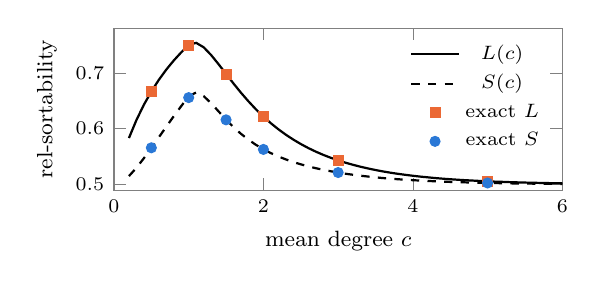
\begin{tikzpicture}
\begin{axis}[width=0.6\textwidth, height=0.3\textwidth, xmin=0, xmax=6, ymin=0.49, ymax=0.78,
  xlabel={mean degree $c$}, ylabel={rel-sortability},
  tick label style={font=\scriptsize}, label style={font=\footnotesize},
  legend style={font=\scriptsize, draw=none, fill=none, at={(0.98,0.97)}, anchor=north east},
  axis line style={gray}, tick style={gray}]
\addplot[thick,black] coordinates {(0.2,0.5833) (0.3,0.6154) (0.4,0.6429) (0.5,0.6667) (0.6,0.6875) (0.7,0.7059) (0.8,0.7222) (0.9,0.7368) (1.0,0.7500) (1.1,0.7538) (1.2,0.7459) (1.3,0.7320) (1.4,0.7155) (1.5,0.6981) (1.6,0.6809) (1.7,0.6644) (1.8,0.6490) (1.9,0.6347) (2.0,0.6217) (2.1,0.6098) (2.2,0.5990) (2.3,0.5893) (2.4,0.5805) (2.5,0.5726) (2.6,0.5654) (2.7,0.5590) (2.8,0.5532) (2.9,0.5480) (3.0,0.5433) (3.1,0.5391) (3.2,0.5353) (3.3,0.5319) (3.4,0.5288) (3.5,0.5260) (3.6,0.5235) (3.7,0.5212) (3.8,0.5192) (3.9,0.5174) (4.0,0.5157) (4.1,0.5142) (4.2,0.5129) (4.3,0.5116) (4.4,0.5105) (4.5,0.5095) (4.6,0.5086) (4.7,0.5078) (4.8,0.5071) (4.9,0.5064) (5.0,0.5058) (5.1,0.5052) (5.2,0.5048) (5.3,0.5043) (5.4,0.5039) (5.5,0.5035) (5.6,0.5032) (5.7,0.5029) (5.8,0.5026) (5.9,0.5024) (6.0,0.5022)};
\addplot[thick,black,dashed] coordinates {(0.2,0.5151) (0.3,0.5299) (0.4,0.5471) (0.5,0.5656) (0.6,0.5846) (0.7,0.6036) (0.8,0.6224) (0.9,0.6405) (1.0,0.6580) (1.1,0.6649) (1.2,0.6584) (1.3,0.6457) (1.4,0.6310) (1.5,0.6163) (1.6,0.6028) (1.7,0.5908) (1.8,0.5803) (1.9,0.5711) (2.0,0.5632) (2.1,0.5563) (2.2,0.5503) (2.3,0.5450) (2.4,0.5403) (2.5,0.5362) (2.6,0.5325) (2.7,0.5293) (2.8,0.5264) (2.9,0.5238) (3.0,0.5214) (3.1,0.5193) (3.2,0.5175) (3.3,0.5158) (3.4,0.5143) (3.5,0.5129) (3.6,0.5116) (3.7,0.5105) (3.8,0.5095) (3.9,0.5086) (4.0,0.5078) (4.1,0.5071) (4.2,0.5064) (4.3,0.5058) (4.4,0.5052) (4.5,0.5047) (4.6,0.5043) (4.7,0.5039) (4.8,0.5035) (4.9,0.5032) (5.0,0.5029) (5.1,0.5026) (5.2,0.5024) (5.3,0.5021) (5.4,0.5019) (5.5,0.5018) (5.6,0.5016) (5.7,0.5014) (5.8,0.5013) (5.9,0.5012) (6.0,0.5011)};

\addplot[only marks, mark=square*, mark size=1.8pt, color={rgb,255:red,235;green,104;blue,52}]
  coordinates {(0.5,0.6666) (1,0.7486) (1.5,0.6975) (2,0.6214) (3,0.5434) (5,0.5059)};
\addplot[only marks, mark=*, mark size=1.8pt, color={rgb,255:red,42;green,120;blue,214}]
  coordinates {(0.5,0.5658) (1,0.6557) (1.5,0.6159) (2,0.5629) (3,0.5215) (5,0.5028)};
\legend{$L(c)$,$S(c)$,exact $L$,exact $S$}
\end{axis}
\end{tikzpicture}
\caption{\cref{prop:er} (lines) against exact computation on seeded graphs
($p=2\cdot10^4$ to $10^5$; points, means over seeds). The standard deviations
over seeds are at most $0.0022$ (\cref{app:er}).}
\label{fig:er}
\end{figure}



\textbf{In-forests (proved identities).} Let the non-loop part be an in-forest
with $m$ edges and $n_1$ nodes with exactly one parent. By
\cref{cor:iff,cor:statiff},
$L=\tfrac12+\frac{m}{2(m+p)}$, $S=\tfrac12+\frac{m-n_1}{2(m+p)}$,
$L-S=\frac{n_1}{2(m+p)}$ (the last checked to machine precision on $18$ random
forests). For a sequence of in-forests with parent-count distribution $\pi$ and
mean $\mu$: $L\to\tfrac12+\frac\mu{2(1+\mu)}$ and
$S\to\tfrac12+\frac{\mu-\pi_1}{2(1+\mu)}$. Exact computation at $p=20{,}000$
(6 seeds each): uniform recursive in-tree ($\pi_1=1/4$, $S\to11/16=0.6875$,
measured $0.68739\pm0.00026$); preferential attachment (measured $\pi_1=0.1656$,
$S=0.70859\pm0.00028$); uniform random labelled tree rooted and oriented to the
root (Poisson(1) parents, $\pi_1\to e^{-1}$, $S\to\tfrac12+(1-e^{-1})/4=0.65803$,
measured $0.65783\pm0.00020$). In all three $L=0.74999$.

\textbf{Directed ER: summary.} $G(p,c/p)$, $m/p\to c$. The finite limit needs
the fraction of non-loop edges inside an SCC ($\to x^2$, the two endpoints lie in
the giant SCC iff the ancestor tree of $i$ and the descendant tree of $j$ are
infinite); the stationary value needs the fraction of up-edges
($\to F_\uparrow$). Both are proved in \cref{app:erproof} below. Large $c$:
$1-x\sim e^{-c}$, $L-\tfrac12\sim e^{-c}$, $S-\tfrac12\sim e^{-c}/2$.

\textbf{Layered DAG (sketch; $L$ proved given edge concentration).} $M$ layers of
width $w$, each node of layer $l+1$ receiving an edge from each node of layer $l$
with probability $c/w$; as $w\to\infty$ with $\mu=c(M-1)/M$,
$L\to\tfrac12+\frac\mu{2(1+\mu)}$ and
$S\to\tfrac12+\frac{\mu(1-e^{-c})}{2(1+\mu)}$. For fixed $w$ and deep $M$ the
stationary value falls below this (observed $0.7824$ against $0.7878$ at
$w=50$, $M=400$, $c=2$); this correction is not derived.

\begin{table}[h]
\caption{Exact computation (means $\pm$ s.d.\ over seeds; SCCs by scipy and source sets by bitsets) against the limits of \cref{prop:er}, proved in \cref{app:erproof}.}
\label{tab:er}
\centering
\begin{tabular}{rrcccc}
\toprule
$c$ & $p$ & $L$ exact & $L$ formula & $S$ exact & $S$ formula \\
\midrule
0.5 & 20000 & $0.6666\pm0.0011$ & $0.6667$ & $0.5658\pm0.0014$ & $0.5656$ \\
1.0 & 20000 & $0.7486\pm0.0008$ & $0.7500$ & $0.6557\pm0.0013$ & $0.6580$ \\
1.5 & 50000 & $0.6975\pm0.0020$ & $0.6981$ & $0.6159\pm0.0018$ & $0.6163$ \\
2.0 & 50000 & $0.6214\pm0.0022$ & $0.6217$ & $0.5629\pm0.0014$ & $0.5632$ \\
3.0 & 100000 & $0.5434\pm0.0010$ & $0.5433$ & $0.5215\pm0.0006$ & $0.5214$ \\
5.0 & 20000 & $0.5059\pm0.0005$ & $0.5058$ & $0.5028\pm0.0003$ & $0.5029$ \\
\bottomrule
\end{tabular}
\end{table}
At the critical point $c=1$, $S$ converges slowly in $p$: $0.65574\pm0.00126$ ($p=2\cdot10^4$, 6 seeds),
$0.65784\pm0.00043$ ($2\cdot10^5$, 6 seeds) and $0.65796$ ($10^6$, 1 seed) against $0.65803$, like $L$
($0.74857$, $0.74972$, $0.74989$ against $0.75$).

$L$ at $c=1$ converges as $p$ grows: $0.7466$ ($p=2000$), $0.7486$ ($2\cdot10^4$),
$0.74976$ ($2\cdot10^5$), $0.74992$ ($10^6$); at $c=2$, $0.62162\pm0.00023$ at
$p=10^6$ against $0.62170$. The giant-SCC fraction matches $x^2$ ($0.6353$ against
$0.6349$ at $c=2$). The second fixed point matters: with $d=1$ the formula would
give $S=0.6312$, $0.5766$, $0.5246$ at $c=1.5,2,3$, outside the error bars,
whereas the fixed points $d=0.485$, $0.221$, $0.061$ give $0.6163$, $0.5632$,
$0.5214$. Further exact rows: $c=1.5$, $p=10^5$, 32 graphs, $L=0.69819\pm0.00024$
(formula $0.69810$); $c=2$, $p=3.2\cdot10^5$, $L=0.62170\pm0.00012$ ($0.62170$).
The Barak--Erd\H{o}s phase-transition paper cited by \citet{reisach2026topological}
concerns monotone-path reachability at the dense scale $\log n/n$ and is not
used here.

\subsection{Directed Erd\H{o}s--R\'enyi summary graphs: full proof of \cref{prop:er}}
\label{app:erproof}

\textbf{Status.} Everything in this subsection is proved on paper. The only
inputs used without proof are textbook facts (F1)--(F3) below, checked against
the author's online version of \citet{hofstad2016random} (theorem numbers are
those of that version and may differ in print). Lemma~\ref{lem:er-local} is the
standard local-coupling argument for sparse random graphs and is written
concisely. The deterministic witness lemmas are machine-checked; no
probabilistic step is. No human probabilist has yet checked this subsection
(see the AI-use statement).

\textbf{Limits and their order.} For a fixed summary graph, \cref{thm:limit}
gives $\lim_{T\to\infty}\srho(\GT)=L(\GS)=\tfrac12+|\Ex|/(2|\Es|)$, and
\cref{thm:stat} gives $\srho^W=\tfrac12+|\Eu|/(2|\Es|)$ for every $T$. For
$\GS\sim D(p,c/p)$ we take the limit $T\to\infty$ at fixed $p$ first (this
defines $L(\GS)$) and then let $p\to\infty$; for the stationary value no
$T$-limit is needed. The regime of fixed $T$ with $p\to\infty$ is not covered
(the bound of \cref{thm:limit} is vacuous for $T\le p$).

\textbf{Model and notation.} $D(p,c/p)$: each ordered pair $(i,j)$, $i\ne j$,
is a non-loop edge independently with probability $q=c/p$, and every node has
a self-loop (loops change neither reachability nor $\Src$). $m$ is the number of
non-loop edges, $|\Es|=p+m$, $N$ the number of non-loop edges inside an SCC, so
$|\Ex|=m-N$. $\mathrm{out}(v)$, $\mathrm{in}(v)$ are the sets of nodes
reachable from $v$, resp.\ reaching $v$ ($v$ included), $T^{\mathrm{out}}_v$,
$T^{\mathrm{in}}_v$ their sizes; $v\leadsto w$ means $w\in\mathrm{out}(v)$.
$x=x(c)$ is the largest solution of $x=1-e^{-cx}$ (the survival probability of
a Poisson$(c)$ Galton--Watson tree), $\theta_K=\theta_K(c)$ the probability that
its total progeny is at least $K$ ($\theta_K\downarrow x$), and $d$ the smallest
fixed point in $[0,1]$ of $f(d)=1+e^{-c}-e^{-c(1-x)d}$. A node is
\emph{in-isolated} if it has no non-loop parent. $\mathcal G$ denotes the
\emph{edge-rooted Poisson tree}: an edge $(i,j)$; $i$ has Poisson$(c)$ parents
and Poisson$(c)$ further children, $j$ Poisson$(c)$ further parents and
Poisson$(c)$ children; every other node has Poisson$(c)$ parents and
Poisson$(c)$ children besides the edge through which it was reached; all
independent.

\textbf{Textbook facts.} (F1) Poisson coupling \citep[Thm.~2.10]{hofstad2016random}:
$d_{\mathrm{TV}}(\mathrm{Bin}(n,q),\mathrm{Poi}(c))\le nq^2+|nq-c|$.
(F2) Chernoff: for a sum $X$ of independent Bernoulli variables with mean
$\mu$ and $\delta\in(0,1)$, $P(X\le(1-\delta)\mu)\le e^{-\delta^2\mu/2}$. (From
$Ee^{-tX}\le\exp(\mu(e^{-t}-1))$ with $t=-\log(1-\delta)$, Markov's inequality,
and $(1-\delta)\log(1-\delta)\ge-\delta+\delta^2/2$; the upper-tail version
$P(X\ge\mu+s)\le e^{-s}$ for $s\ge e^2\mu$ follows in the same way.)
(F3) Galton--Watson facts \citep[Thms.~3.1, 3.16]{hofstad2016random}: the
extinction probability is the smallest root of $\eta=e^{c(\eta-1)}$, so the
survival probability is $x(c)$, positive iff $c>1$.

\textbf{Deterministic lemmas} (machine-checked, \lname{ErLemmas.lean}; no loop
hypothesis). A node $z$ is a \emph{source node} if every ancestor of $z$ is
reachable from $z$. By \cref{thm:stat}, $(i,j)\in\Eu$ iff some source node
reaches $j$ but not $i$.
\begin{itemize}
\item[(W1)] If $(i,j)\in\Eu$, there are $k\notin\{i,j\}$ with $k\to j$ and a
source node $z$ with $z\leadsto k$, $z\not\leadsto i$ (\lname{upEdge_witness}).
\item[(W2)] If $i\to j$, $k\to j$, and a source node reaches $k$ but not $i$,
then $(i,j)\in\Eu$ (\lname{mem_upEdges_of_witness}).
\item[(W3)] If $i\to j$, $k\to j$ and $\mathrm{in}(k)\cap\mathrm{in}(i)=\emptyset$,
then $(i,j)\in\Eu$ (\lname{mem_upEdges_of_disjoint_anc}).
\item[(W5)] A non-loop edge $(i,j)$ lies inside an SCC iff $j\leadsto i$. The
event $\{j\leadsto i\}$ and the set $\mathrm{out}(j)$ do not change when the
edge $(i,j)$ is added or removed (a simple path from $j$ to $i$ does not use
it). (Trivial; not formalised.)
\end{itemize}

\textbf{Explorations and forced edges.} Forward exploration of $\mathrm{out}(v)$
keeps explored, active and unseen sets $X_t,A_t,U_t$, $a_t=|A_t|$,
$\mathrm{disc}_t=t+a_t$, $X_0=\emptyset$, $A_0=\{v\}$. Step $t+1$ takes the
oldest active node $w$, reveals the pairs $(w,u)$, $u\in U_t$, and makes the
$\xi_{t+1}$ heads of present pairs active; it stops at $T=T^{\mathrm{out}}_v$.
Backward exploration of $\mathrm{in}(v)$ reveals the pairs $(u,w)$ instead.
Let $F$ be a set of at most three ordered pairs and $G^F$ the graph in which the
pairs of $F$ are present and all other pairs are independent Be$(q)$.
\emph{Bookkeeping.} In a forward exploration a pair is revealed only when its
tail is explored, and each node is explored once, so each pair is revealed at
most once; the pairs revealed at step $t+1$ are disjoint from those revealed
before and from all pairs whose tail is not in $X_{t+1}$. Hence, conditionally
on the history $\mathcal H_t$, the non-forced pairs revealed at step $t+1$ are
independent Be$(q)$, and
$\xi_{t+1}=\#\{u\in U_t:(w,u)\in F\}+\mathrm{Bin}(|U_t|-f_w,q)$ with
$f_w\le3$ the number of forced pairs from $w$ into $U_t$. Thus, given
$\mathcal H_t$, $\xi_{t+1}$ stochastically dominates $\mathrm{Bin}(|U_t|-3,q)$
and is dominated by $3+\mathrm{Bin}(p,q)$. The same holds for backward
explorations (with heads in place of tails), and, by the same argument, for a
backward exploration run after a forward one, conditionally on the forward
history, as long as it never discovers a node that the forward exploration
discovered (only pairs with tail outside $X_f$ and head explored backward are
revealed, and none of them was revealed forward).

Fix $c>1$ and $\varepsilon\in(0,1/5)$ with $\beta=c(1-4\varepsilon)>1$; put
$n'=\lceil(1-4\varepsilon)p\rceil$, $\kappa=(\beta-1)^2/(8\beta)$,
$\delta=(\beta-1)\varepsilon/(\beta+1)$, $t_0=C_3\log p$ with $C_3\kappa\ge8$.
Call an exploration \emph{admissible} if, conditionally on its history, every
offspring count $\xi_{t+1}$ taken while $\mathrm{disc}_t<\varepsilon p$
dominates $\mathrm{Bin}(n',q)$ and every offspring count is dominated by
$3+\mathrm{Bin}(p,q)$. By the bookkeeping, forward and backward explorations in
$G^F$ are admissible for large $p$ (since $|U_t|-3>(1-\varepsilon)p-3\ge n'$),
and so is the backward exploration of Lemma~\ref{lem:er-l2} below.

\begin{lemma}[dichotomy]\label{lem:er-l1}
There is $C$ (depending on $c,\varepsilon$) such that for large $p$ every
admissible exploration with final size $T$ satisfies
(a) $P(K\le T<\varepsilon p)\le Ce^{-\kappa K}$ for all $K\ge1$;
(b) $P\big(T\ge t_0$ and [$\mathrm{disc}_t<\varepsilon p$ for all $t$, or
$a_\tau<\delta p$ at $\tau=\min\{t:\mathrm{disc}_t\ge\varepsilon p\}$]$\big)\le Cp^{-8}$.
Consequently, with probability at least $1-Cp^{-7}$, every node $v$ of $G$ has, in
both directions, $T_v<t_0$ or ($T_v\ge\varepsilon p$ and $a_\tau\ge\delta p$).
\end{lemma}
\begin{proof}
Let $\xi'_t$ be independent $\mathrm{Bin}(n',q)$ variables coupled so that
$\xi_t\ge\xi'_t$ for $t\le\tau$ (admissibility; after $\tau$ or after the
exploration stops, $\xi'_t$ uses external randomness), and
$W_t=1+\sum_{s\le t}(\xi'_s-1)$. By induction $a_t\ge W_t$ for
$t\le\min(T,\tau)$. Since $tn'q\ge t\beta$ and
$(\beta+1)/2=(1-\frac{\beta-1}{2\beta})\beta$, (F2) gives
$P(W_t\le(\beta-1)t/2)\le P(\mathrm{Bin}(tn',q)\le t(\beta+1)/2)\le e^{-\kappa t}$,
so $\mathrm{Bad}(t_1)=\{\exists t\ge t_1:W_t\le(\beta-1)t/2\}$ has probability at
most $e^{-\kappa t_1}/(1-e^{-\kappa})$.
(a) If $T<\varepsilon p$ then $\tau=\infty$, so $0=a_T\ge W_T$, which is
$\mathrm{Bad}(K)$ when $T\ge K$.
(b) On $\mathrm{Bad}(t_0)^c$ with $T\ge t_0$: for $t_0\le t\le\min(T,\tau)$,
$a_t\ge W_t>0$, so the exploration cannot stop before $\tau$, hence
$\tau<\infty$. At $\tau$, $a_\tau+\tau\ge\varepsilon p$, and if $\tau\ge t_0$
also $a_\tau>(\beta-1)\tau/2$; minimising $\max((\beta-1)\tau/2,\varepsilon p-\tau)$
over $\tau$ gives $a_\tau\ge\delta p$; if $\tau<t_0$, $a_\tau\ge\varepsilon p-t_0\ge\delta p$.
$e^{-\kappa t_0}\le p^{-8}$. The consequence is a union bound over $p$ nodes and
two directions.
\end{proof}

\begin{lemma}[large out-sets reach large in-sets]\label{lem:er-l2}
With probability at least $1-Cp^{-5}$: for all $v,w$, $T^{\mathrm{out}}_v\ge t_0$
and $T^{\mathrm{in}}_w\ge t_0$ imply $v\leadsto w$.
\end{lemma}
\begin{proof}
Fix $(v,w)$. Explore $\mathrm{out}(v)$ forward up to $\tau_f$ (history $\mathcal H_f$,
discovered set $R_f=X_f\cup A_f$). Since every $\xi$ is dominated by
$3+\mathrm{Bin}(p,q)$, $P(\max_t\xi_t\ge\varepsilon p)\le e^{-\varepsilon p}$ for
large $p$ (F2, upper tail), so $|R_f|\le2\varepsilon p$ except on that event.
Then explore $\mathrm{in}(w)$ backward, stopping at $\tau_b$ or when a node of
$R_f\subseteq\mathrm{out}(v)$ is discovered; in the latter case $v\leadsto w$.
Otherwise the backward exploration is the true exploration of $\mathrm{in}(w)$,
its unseen set has at least $p-2\varepsilon p-\varepsilon p-3\ge n'$ usable
nodes while $\mathrm{disc}<\varepsilon p$, and by the bookkeeping it is admissible
conditionally on $\mathcal H_f$. By Lemma~\ref{lem:er-l1}(b) for both
explorations, outside probability $2Cp^{-8}$: if $T^{\mathrm{out}}_v,T^{\mathrm{in}}_w\ge t_0$
and no connection occurred, then $|A_f|,|A_b|\ge\delta p$. $A_f$ and $A_b$ are
disjoint, and every pair $(a,a')\in A_f\times A_b$ is unrevealed (its tail is not
in $X_f$, its head not in $X_b$), so given both histories these pairs are
independent Be$(q)$ (or forced present): $P(\text{no edge }A_f\to A_b)\le(1-q)^{\delta^2p^2-3}\le e^{-c\delta^2p/2}$.
An edge $a\to a'$ gives $v\leadsto a\to a'\leadsto w$. Union bound over $p^2$
pairs.
\end{proof}

Let $\Omega$ be the intersection of the events of Lemma~\ref{lem:er-l1}
(consequence) and Lemma~\ref{lem:er-l2}, $P(\Omega^c)\le Cp^{-5}$. Put
$\mathcal S=\{v:T^{\mathrm{out}}_v\ge t_0\}$, $\mathcal T=\{v:T^{\mathrm{in}}_v\ge t_0\}$.

\begin{corollary}[structure]\label{cor:er-struct}
On $\Omega$: $\mathcal S\times\mathcal T$ is contained in the reachability
relation; every SCC other than the one containing $\mathcal S\cap\mathcal T$ has
fewer than $t_0$ nodes; if $|\mathcal S\cap\mathcal T|\ge t_0$, this SCC equals
$\mathcal S\cap\mathcal T$.
\end{corollary}
\begin{proof}
The first claim is Lemma~\ref{lem:er-l2}. A node $u\notin\mathcal S\cap\mathcal T$
has $T^{\mathrm{out}}_u<t_0$ or $T^{\mathrm{in}}_u<t_0$, and its SCC lies in
$\mathrm{out}(u)\cap\mathrm{in}(u)$. If $u$ were in the SCC of
$\mathcal S\cap\mathcal T$, that SCC (of size $\ge t_0$) would lie in
$\mathrm{out}(u)\cap\mathrm{in}(u)$, a contradiction.
\end{proof}
(This re-proves the part of the Karp--{\L}uczak structure theorem we need; the
statement is recorded in the introduction of \citealp{dovgal2020birth}.)

\begin{lemma}[local concentration; standard coupling]\label{lem:er-local}
Fix $R$ and a function $\varphi$ of the isomorphism class of the radius-$R$
neighbourhood $B_R(e)$ of a non-loop edge $e$ (all edges incident to nodes at
undirected distance $<R$ from $e$, rooted at the oriented edge $e$), and let
$\Phi_p=p^{-1}\sum_e\varphi(B_R(e))$, the sum over non-loop edges.
(a) If $\varphi$ is bounded, $E\Phi_p\to cE_{\mathcal G}\varphi$ and
$\mathrm{Var}\,\Phi_p\to0$; the same holds for node-rooted functionals with the
node-rooted Poisson tree.
(b) If $\varphi\ge0$ and $\varphi(B_R(e))\le\mathrm{indeg}(j)$ for $e=(i,j)$, then
$\limsup_pE\Phi_p\le cE_{\mathcal G}[\min(\varphi,M)]+C/M$ for every $M$, with $C$
not depending on $p$ or $M$.
\end{lemma}
\begin{proof}
(a) First moment:
$E\sum_e\varphi(B_R(e))=\sum_{(i,j)}q\,E[\varphi(B_R((i,j);G\cup\{(i,j)\}))]$.
Explore the undirected neighbourhood of $(i,j)$ breadth first, revealing for
each explored node $w$ all pairs $(w,u)$ and $(u,w)$. On $\{|B_R|\le M\}$, each
explored node has $\mathrm{Bin}(|U|,q)$ new children and $\mathrm{Bin}(|U|,q)$
new parents among the unseen nodes, $|U|\ge p-M$, which (F1) couples with
Poisson$(c)$ up to an error $\le Mq^2p+cM/p$ per count, and the pairs between
already seen nodes are present with total probability $\le M^2q$. So the
truncated ball is within $C(M,R)/p$ in total variation of the truncated
$\mathcal G$. Tightness: each exploration step is dominated by
$\mathrm{Bin}(2p,q)$ (resp.\ Poisson$(2c)$), so $E|B_R|\le(1+2c+o(1))^R$ and
$P(|B_R|>M)\le C^R/M$ uniformly in $p$; let $p\to\infty$, then $M\to\infty$.
Second moment: $E\Phi_p^2=p^{-2}\big[\sum_e+\sum_{e,f\text{ sharing a node}}+\sum_{e,f\text{ node-disjoint}}\big]$.
The first two sums are $O(p)$ since $E\sum_vd(v)^2=O(p)$. For node-disjoint
$e,f$, explore both balls jointly in $G\cup\{e,f\}$: on $\{$both sizes $\le M\}$
they are disjoint and non-adjacent except with probability $\le C(M,R)/p$, and
then the two explorations are coupled with independent copies of $\mathcal G$.
Hence $p^{-2}\sum_{\text{disjoint}}\to(cE_{\mathcal G}\varphi)^2$ and
$\mathrm{Var}\,\Phi_p\to0$.
(b) Apply (a) to $\min(\varphi,M)$ and bound the rest by
$E\sum_{(i,j)}\mathrm{indeg}(j)\mathbf 1[\mathrm{indeg}(j)>M]=E\sum_j\mathrm{indeg}(j)^2\mathbf 1[\mathrm{indeg}(j)>M]\le p\,E[D^3]/M$,
$D\sim\mathrm{Bin}(p-1,q)$, and $E[D^3]\le c^3+3c^2+c$ for all $p$ (uniform
integrability).
\end{proof}

\textbf{Local functionals.} All of the following are functions of $B_{2K+1}(e)$
(a breadth-first search of the first $K$ nodes of a set stays within distance
$K-1$), are invariant under isomorphism, and count all qualifying nodes, so no
labelling enters.
$A^K_e=\mathbf 1[T^{\mathrm{out}}_j\ge K,\ T^{\mathrm{in}}_i\ge K]$, with
$E_{\mathcal G}A^K=\theta_K^2$ (the descendant tree of $j$ and the ancestor tree
of $i$ are independent Poisson Galton--Watson trees).
$\Psi_K(e)=\mathrm{cl}_1\vee\mathrm{cl}_2$, with
$\mathrm{cl}_1=[T^{\mathrm{in}}_i<K$ and $j$ has a parent $k\notin\{i,j\}]$ and
$\mathrm{cl}_2=[$some in-isolated $s$ has $T^{\mathrm{out}}_s<K$, $j\in\mathrm{out}(s)$, $i\notin\mathrm{out}(s)]$.
$\varphi^{\beta}_K(e)=\#\{k\notin\{i,j\}:k\to j,\ T^{\mathrm{in}}_k<K,\ T^{\mathrm{in}}_i<K,\ \mathrm{in}(k)\cap\mathrm{in}(i)\ne\emptyset\}\le\mathrm{indeg}(j)$,
with $E_{\mathcal G}\min(\varphi^\beta_K,M)=0$ (in $\mathcal G$ the ancestor trees
of $i$ and of another parent of $j$ are disjoint).

\begin{proposition}[$L$, $c>1$]\label{prop:er-N}
For $c>1$, $N/p\to cx^2$ in $L^1$ and in probability.
\end{proposition}
\begin{proof}
By (W5), $N=\sum_eZ_e$ with $Z_e=\mathbf 1[j\leadsto i]$; compare with
$\tilde N_K=\sum_eA^K_e$.
(i) $Z=1,A=0$: $j\leadsto i$ and ($T^{\mathrm{out}}_j<K$ or $T^{\mathrm{in}}_i<K$).
By (W5) these events do not depend on the presence of $e$, so the expected
number of such edges is $p(p-1)q\,P(i\in\mathrm{out}(j),T^{\mathrm{out}}_j<K)$ plus
the same with $\mathrm{in}(i)$, and by exchangeability of the $p-1$ nodes other
than $j$, $P(i\in\mathrm{out}(j),T^{\mathrm{out}}_j<K)=E[(T^{\mathrm{out}}_j-1)\mathbf 1(T^{\mathrm{out}}_j<K)]/(p-1)\le K/(p-1)$.
Total $\le2cK$.
(ii) $Z=0,A=1$: on $\Omega$, $T^{\mathrm{out}}_j\ge t_0$ and $T^{\mathrm{in}}_i\ge t_0$
would give $j\leadsto i$, so $T^{\mathrm{out}}_j$ or $T^{\mathrm{in}}_i$ lies in
$[K,t_0)\subseteq[K,\varepsilon p)$. The expected number of such edges is at
most $\sum_{(i,j)}q\,P_{G^{\{e\}}}(\cdot)\le cp\cdot2Ce^{-\kappa K}$ by
Lemma~\ref{lem:er-l1}(a) in $G^{\{e\}}$; on $\Omega^c$ the count is at most $m$
and $E[m\mathbf 1_{\Omega^c}]\le(Em^2)^{1/2}P(\Omega^c)^{1/2}=O(p\cdot p^{-5/2})$.
So $E|N-\tilde N_K|\le2cK+2cCpe^{-\kappa K}+o(1)$. By
Lemma~\ref{lem:er-local}(a), $\tilde N_K/p\to c\theta_K^2$ in $L^2$; hence
$\limsup_pE|N/p-cx^2|\le2cCe^{-\kappa K}+c|\theta_K^2-x^2|\to0$ as $K\to\infty$.
\end{proof}
The same argument for the node functional $\mathbf 1[T^{\mathrm{out}}_v\ge K,T^{\mathrm{in}}_v\ge K]$
gives $|\mathcal S\cap\mathcal T|/p\to x^2$, so by \cref{cor:er-struct} the giant
SCC has $(x^2+o_P(1))p$ nodes and all other SCCs fewer than $C_3\log p$, w.h.p.

\begin{proposition}[the tree computation]\label{prop:er-tree}
In $\mathcal G$, with $\Psi_\infty$ defined by $T^{\mathrm{in}}_i<\infty$ and
$T^{\mathrm{out}}_s<\infty$, $E_{\mathcal G}\Psi_K\uparrow P_{\mathcal G}(\Psi_\infty)=F_\uparrow$
as $K\to\infty$.
\end{proposition}
\begin{proof}
Both clauses increase in $K$ to their $K=\infty$ versions (monotone convergence).
Let $A(i)$ be the event that the ancestor tree of $i$ is infinite and $D(j)$ that
the descendant tree of $j$ is infinite (probability $x$ each, independent). The
other parents of $j$ are Poisson$(c)$ many.
(1) Not $A(i)$: $\Psi_\infty$ holds iff $j$ has another parent. Clause 1 needs
exactly that; clause 2 needs it too, since a path from $s$ to $j$ ends with an
edge $k\to j$ and $k=i$ would put $i$ into $\mathrm{out}(s)$. Probability
$(1-x)(1-e^{-c})$.
(2) $A(i)$: clause 1 fails. Clause 2 needs (a) not $D(j)$, since
$\mathrm{out}(s)$ contains the descendant tree of $j$ (probability $1-x$), and
(b) another parent $k$ of $j$ and a chain $k=u_0\leftarrow u_1\leftarrow\dots\leftarrow u_r=s$
ending at an in-isolated $s$, in which every $u_t$ has only finite descendant
trees below its children other than $u_{t-1}$ ($u_{-1}=j$); such an $s$ does not
reach $i$, because paths into $i$ stay in the ancestor tree of $i$. The
probability that all other children of a node have finite descendant trees is
$E[(1-x)^{\mathrm{Poi}(c)}]=e^{-cx}=1-x$. Let $Q(v)$ be the event that $v$ is
in-isolated or some parent $u$ of $v$ has all other children finite and $Q(u)$
holds, and $d^*=P(Q)$. Parents are Poisson$(c)$ many and each is \emph{good}
(other children finite and $Q$) independently with probability $(1-x)d^*$, so by
Poisson thinning $d^*=e^{-c}+1-e^{-c(1-x)d^*}=f(d^*)$. $Q$ is the increasing
union of its depth-$n$ truncations $Q_n$, with $P(Q_0)=e^{-c}=f(0)$ and
$P(Q_{n+1})=f(P(Q_n))$; as $f$ is increasing and continuous, $P(Q_n)=f^{n+1}(0)$
increases to the smallest fixed point $d$ of $f$ (if $d'$ is a fixed point,
$f^n(0)\le f^n(d')=d'$). So $d^*=d$. The number of good other parents of $j$ is
Poisson$(c(1-x)d)$, so (b) has probability $1-e^{-c(1-x)d}$, independently of
$A(i)$ and $D(j)$. Adding (1) and (2) gives $F_\uparrow$.
\end{proof}
(An independent Monte Carlo of the event itself, not of the closed form, gives
$0.38756\pm0.00077$ against $0.38773$ at $c=1.5$ and $0.19049\pm0.00062$ against
$0.18962$ at $c=2$.)

\begin{proposition}[reduction of $\Eu$ to $\Psi_K$, $c>1$]\label{prop:er-red}
$E\sum_e|\mathbf 1[e\in\Eu]-\Psi_K(e)|\le(\delta_1(K)+o(1))p$ with
$\delta_1(K)=C(c^2+K^2)e^{-\kappa K}+o_K(1)$, where $o_K(1)\to0$ as $K\to\infty$
and $C$ does not depend on $K$ or $p$.
\end{proposition}
\begin{proof}
Let $e=(i,j)$ be a non-loop edge. \emph{Clause 2 never errs}: an in-isolated $s$
is a source node, so $j\in\mathrm{out}(s)$, $i\notin\mathrm{out}(s)$ give
$e\in\Eu$. \emph{Case I: $T^{\mathrm{in}}_i<K$.} (I-a) If $e\in\Eu$, (W1) gives
another parent of $j$, so clause 1 holds: no error. (I-b) Clause 1 holds and
$e\notin\Eu$. Then
$\mathbf 1[\text{I-b}]\le\sum_{k\notin\{i,j\}}\mathbf 1[e,(k,j)\text{ present},\ T^{\mathrm{in}}_i<K,\ e\notin\Eu]$
(a union over \emph{all} other parents; no parent is singled out). Fix the
triple $(i,j,k)$ and force $F=\{(i,j),(k,j)\}$. By (W3), $e\notin\Eu$ forces
$\mathrm{in}(k)\cap\mathrm{in}(i)\ne\emptyset$, and by (W2) every source node
reaching $k$ reaches $i$. Split on $T^{\mathrm{in}}_k$:
($\alpha_1$) $K\le T^{\mathrm{in}}_k<\varepsilon p$: probability $\le Ce^{-\kappa K}$
(Lemma~\ref{lem:er-l1}(a), backward, in $G^F$).
($\alpha_2$) $T^{\mathrm{in}}_k\ge\varepsilon p$: the backward exploration of
$\mathrm{in}(k)$ explores at least $\varepsilon p/2$ nodes. When a node $y\ne j$ is
explored, the pairs $(u,y)$ with $u$ unseen are revealed (all absent with
conditional probability $\ge(1-q)^p$), and the pairs $(u,y)$ with $u$ already
seen are never revealed by this exploration and are independent of it and of
each other (distinct heads); so, given the history, $y$ is in-isolated with
probability $\ge(1-q)^p\ge e^{-c}/2$, and the number of in-isolated nodes among
the first $\varepsilon p/2$ explored nodes dominates
$\mathrm{Bin}(\varepsilon p/2-1,e^{-c}/2)$. By (F2) at least $K$ of them are
in-isolated except with probability $e^{-\Omega(p)}$. Each in-isolated node of
$\mathrm{in}(k)$ is a source node reaching $k$, hence reaches $i$, so lies in
$\mathrm{in}(i)$; but $|\mathrm{in}(i)|<K$. So ($\alpha_2$) has probability
$e^{-\Omega(p)}$.
($\beta$) $T^{\mathrm{in}}_k<K$ and $\mathrm{in}(k)\cap\mathrm{in}(i)\ne\emptyset$.
Summed over $k$ this is $\varphi^\beta_K(e)$.
The number of triples is $p^3$ and each has both pairs present with probability
$q^2$, so cases ($\alpha_1$), ($\alpha_2$) contribute at most
$c^2p(Ce^{-\kappa K}+e^{-\Omega(p)})$; case ($\beta$) contributes
$E\sum_e\varphi^\beta_K(e)\le(C/M+o(1))p$ for every $M$ by
Lemma~\ref{lem:er-local}(b), i.e.\ $o(p)$.
\emph{Case II: $T^{\mathrm{in}}_i\ge K$.} Clause 1 fails.
(II-0) $K\le T^{\mathrm{in}}_i<\varepsilon p$: at most $cpCe^{-\kappa K}$ such
edges in expectation (Lemma~\ref{lem:er-l1}(a) in $G^{\{e\}}$).
(II-1) $T^{\mathrm{in}}_i\ge\varepsilon p$, so $i\in\mathcal T$. Work on
$\Omega'=\Omega\cap\{\max_v\mathrm{indeg}(v)\le C\log p\}$; $P(\Omega'^c)\le Cp^{-2}$,
and the edges counted on $\Omega'^c$ contribute at most
$E[m\mathbf 1_{\Omega'^c}]\le(Em^2)^{1/2}P(\Omega'^c)^{1/2}=O(1)$. An error here is
an edge $e\in\Eu$ with $\Psi_K(e)=0$. Take a witness source node $z$ of (W1),
in a source SCC $\sigma$. On $\Omega$, $z\in\mathcal S$ would give $z\leadsto i$
(Lemma~\ref{lem:er-l2}), so $T^{\mathrm{out}}_z<t_0$.
(A) $\sigma=\{z\}$ (i.e.\ $z$ in-isolated) and $T^{\mathrm{out}}_z<K$: clause 2
holds with $s=z$; no error.
(B1) $z$ in-isolated and $K\le T^{\mathrm{out}}_z<t_0$. The number of such edges
is at most $\sum_z\mathbf 1[K\le T^{\mathrm{out}}_z<t_0]\sum_{j\in\mathrm{out}(z)}\mathrm{indeg}(j)$.
Given $\mathrm{out}(z)=O$ with $|O|=r$ (a completed forward exploration), the
pairs with tail outside $O$ and head in $O$ are unrevealed, so the expected
number of edges into $O$ is at most $r^2+rpq=r^2+cr$. With
$P(T^{\mathrm{out}}_z=r)\le Ce^{-\kappa r}$ (Lemma~\ref{lem:er-l1}(a)), the
expectation is at most $p\sum_{r\ge K}Ce^{-\kappa r}(r^2+cr)\le C'pK^2e^{-\kappa K}$.
(B2) $|\sigma|\ge2$. Then $|\sigma|<t_0$ (as $\sigma\subseteq\mathrm{out}(z)$),
every node of $\sigma$ has out-set $\mathrm{out}(z)$ of size $<t_0$, and the
number of edges with head in $\mathrm{out}(z)$ is at most $t_0\cdot C\log p$ on
$\Omega'$. Let $N_\sigma$ be the number of source SCCs with $2\le|\sigma|<t_0$.
For a set $R$ of size $r$, ``$R$ strongly connected'' and ``no edge enters $R$''
depend on disjoint sets of pairs; the first requires every node of $R$ to have
a parent in $R$ (probability $\le(rq)^r$, distinct heads), the second has
probability $(1-q)^{r(p-r)}$. Hence
$EN_\sigma\le\sum_{r=2}^{t_0}\binom pr(rq)^r(1-q)^{r(p-r)}\le\sum_{r\ge2}\big(ce^{1-c}e^{cr/p}\big)^r=O(1)$,
using $\binom pr\le p^r/r!$, $r^r/r!\le e^r$, $r\le t_0=O(\log p)$ and
$ce^{1-c}<1$ for $c\ne1$. So the (B2) errors have expectation
$O(1)\cdot t_0C\log p=O(\log^2p)=o(p)$: an expectation on the event $\Omega'$ plus
the Cauchy--Schwarz bound for $\Omega'^c$ above.
Adding all cases gives the claim.
\end{proof}

\begin{theorem}[$S$, $c>1$]\label{thm:er-S}
For $c>1$, $|\Eu|/p\to cF_\uparrow$, and therefore
$S=\tfrac12+|\Eu|/(2(p+m))\to\tfrac12+cF_\uparrow/(2(1+c))$, in $L^1$ and in
probability.
\end{theorem}
\begin{proof}
$E\big||\Eu|/p-cF_\uparrow\big|\le E\sum_e|\mathbf 1[e\in\Eu]-\Psi_K(e)|/p+E|\Phi^{\Psi_K}_p-cE_{\mathcal G}\Psi_K|+c|E_{\mathcal G}\Psi_K-F_\uparrow|$;
the terms are bounded by Prop.~\ref{prop:er-red}, Lemma~\ref{lem:er-local}(a) and
Prop.~\ref{prop:er-tree}; let $p\to\infty$, then $K\to\infty$. $m/p\to c$ in
$L^2$ ($m\sim\mathrm{Bin}(p(p-1),q)$), and $S$ and $L$ are bounded continuous
functions of $(|\Eu|/p,m/p)$ and $(N/p,m/p)$ on $[0,\infty)^2$.
\end{proof}

\begin{proposition}[$c\le1$]\label{prop:er-sub}
(a) For $c<1$, $EN\le c^2/(1-c)$. (b) For $c\le1$, $N/p\to0$ in $L^1$, so
$L\to\tfrac12+\frac{c}{2(1+c)}$ ($L(1)=3/4$). (c) For $c\le1$,
$|\Eu|/p\to c(1-e^{-c})$ in $L^1$, so $S\to\tfrac12+\frac{c(1-e^{-c})}{2(1+c)}$
($S(1)=0.65803$); this is $F_\uparrow$ at $x=0$.
\end{proposition}
\begin{proof}
(a) A non-loop edge inside an SCC lies on a simple directed cycle, and the
expected number of pairs (simple cycle of length $k$, edge on it) is
$k\cdot\frac{(p)_k}{k}q^k\le c^k$; sum over $k\ge2$.
(b) $c<1$ from (a). $c=1$: $D(p,1/p)$ is a subgraph of $D(p,c'/p)$ for every
$c'>1$ under the monotone coupling, and an edge inside an SCC of the subgraph is
inside an SCC of the larger graph, so $\limsup_pEN/p\le c'x(c')^2\to0$ as
$c'\downarrow1$ (Prop.~\ref{prop:er-N}).
(c) Let $\Psi^1_K=\mathrm{cl}_1$. Case I ($T^{\mathrm{in}}_i<K$): (I-a) as before,
no error; (I-b) with the same union over other parents $k$ and forced
$F=\{(i,j),(k,j)\}$, (W3) forces $\mathrm{in}(k)\cap\mathrm{in}(i)\ne\emptyset$,
so either $T^{\mathrm{in}}_k\ge K$ or the event of $\varphi^\beta_K$ holds. The
expected number of triples with $T^{\mathrm{in}}_k\ge K$ is
$E\sum_e\#\{k\notin\{i,j\}:k\to j,\ T^{\mathrm{in}}_k\ge K\}$, a local functional
dominated by $\mathrm{indeg}(j)$, so by Lemma~\ref{lem:er-local}(b) it is at most
$(c\cdot c\,\theta_K+C/M+o(1))p$; the $\varphi^\beta_K$ part is $o(p)$ as before.
Case II ($T^{\mathrm{in}}_i\ge K$): at most $E\sum_e\mathbf 1[T^{\mathrm{in}}_i\ge K]=(c\theta_K+o(1))p$
(Lemma~\ref{lem:er-local}(a)). Hence
$\limsup_pE\sum_e|\mathbf 1[e\in\Eu]-\Psi^1_K(e)|/p\le c^2\theta_K+c\theta_K+C/M$, which
tends to $0$ as $K,M\to\infty$ because $\theta_K\to x(c)=0$ for $c\le1$ (F3).
Finally $E_{\mathcal G}\Psi^1_K=(1-\theta_K)(1-e^{-c})\to1-e^{-c}$.
\end{proof}

\textbf{What is not proved.} Rates of convergence; the critical window
$c=1+\lambda p^{-1/3}$ (\L{}uczak and Seierstad, recorded in
\citealp{dovgal2020birth}; not used); almost sure convergence; the regime of
fixed $T$ with $p\to\infty$. The proof does not use the structure theorems of
Karp and of \L{}uczak (not opened by us); it re-proves the part it needs.

\textbf{Numerical checks of the intermediate claims} (fixed seeds, exact
computation; supplement \texttt{x1proof/verify}). (W4) $\Eu\subseteq$ edges into
confluences: 0 violations in 48 graphs. Dichotomy (Lemma~\ref{lem:er-l1}): at
$c=2$, $p=10^5$, the mass of $K\le T<0.02p$ is $0.0097$, $0.0008$, $0$ for
$K=5,10,20$; at $c=1$ it is $0.37$, $0.25$, $0.17$ (critical, no dichotomy, as
expected). Structure (\cref{cor:er-struct}): for $c\ge1.5$ the second-largest
SCC never had more than 2 nodes; giant fraction $0.63439$ ($p=10^6$, $c=2$)
against $x^2=0.63491$. Prop.~\ref{prop:er-red} edge by edge: at $c=2$,
$p=2\cdot10^5$, $|\Eu|=76{,}220$ and $\sum_e\Psi_{40}(e)=76{,}220$ with no edge
in either difference; clause 2 never erred in any run. Concentration: the
standard deviation of $N/p$ times $\sqrt p$ is $2.88$--$3.07$ for
$p=5\cdot10^3$ to $3.2\cdot10^5$ ($c=2$), as Lemma~\ref{lem:er-local} requires.

%=============================================================================
\section{Accuracy Interpretation of $\srho$}
\label{app:x3}

An edge $\{x,y\}$ of a DAG is shown in a uniformly random order together with
$(\rho_{\mathrm{first}},\rho_{\mathrm{second}})$. A \emph{pairwise count rule} is
$f(a,b)\in[0,1]$, the probability of declaring ``first is the tail''; the
\emph{sort rule} is $f_{\mathrm{sort}}=1,\tfrac12,0$ for $a<,=,>b$. For the true
edge $x\to y$ the accuracy is $\tfrac12f(\rho_x,\rho_y)+\tfrac12(1-f(\rho_y,\rho_x))$.

\begin{proposition}[elementary]\label{prop:x3}
On every DAG, (i) the accuracy of $f_{\mathrm{sort}}$ is exactly $\srho$;
(ii) every pairwise count rule has accuracy at most $\srho$; (iii)
$f_{\mathrm{sort}}$ never errs on an edge with $\rho_x\ne\rho_y$.
\lean{\lname{accRule_sortRule}, \lname{accRule_sortRule_rho}, \lname{accRule_le_sOf}, \lname{accRule_le_sRho}, \lname{edgeAcc_sortRule_strict}, \lname{rho_not_gt_of_edge}.}
\end{proposition}
\begin{proof}
By Reisach et al.'s Theorem~1, $\rho_x\le\rho_y$ on an edge $x\to y$. If
$\rho_x<\rho_y$ the accuracy is at most $1$, attained by the sort rule; if
$\rho_x=\rho_y=a$ it is $\tfrac12f(a,a)+\tfrac12(1-f(a,a))=\tfrac12$ for every
$f$, because the random order forces the tie decision to $1/2$. These are the edge
scores. (i) restates the definition of $\srho$; (ii) is a three-line consequence of
their Theorem~1.
\end{proof}
Combined with \cref{thm:stat}, the best accuracy of any pairwise count rule on the
stationary unrolled DAG is $\tfrac12+|\Eu|/(2|\Es|)$, at most $0.665$ for ER
summary graphs and $0.75$ for river-like in-forests ($\mu\le1$). The restriction
to counts is necessary (exhaustive enumeration over labelled DAGs, not proved):

\begin{center}\small
\begin{tabular}{lcccc}
\toprule
nodes $p$ & 2 & 3 & 4 & 5 \\
\midrule
Bayes rule on the two counts (= edge-pooled $\srho$) & 0.5 & 0.5625 & 0.592262 & 0.605547 \\
Bayes rule on counts and the two node degrees & 0.5 & 0.625 & 0.660714 & 0.669238 \\
\bottomrule
\end{tabular}
\end{center}
For the skeleton $a-c-b$ the collider has counts $(2,2,3)$ (all edges strict)
while the chain and the fork have all counts equal to $3$; among the tied graphs the
centre $c$ is the tail with probability $2/3$ under a uniform prior, so a
degree-aware rule beats the coin. So $\srho$ is the Bayes accuracy of pairwise
count rules only. This section is interpretive, not a new theorem.

\section{Benchmark Experiment B1: Design, Results and Deviations}
\label{app:b1}


\textbf{Process.} The analysis plan (\texttt{b1/PLAN.md}) was committed before
any simulation that produced an algorithm score; only graph-only exact values
were computed before it. Two deviations were recorded in the plan after the
validation run (seeds 9000--9004, used only for debugging and timing) and
before the test run: D1, the burn-in was raised from 50 to 100 steps because
the validation mixing check failed (error $2.8\cdot10^{-3}$, threshold
$10^{-3}$; $1.4\cdot10^{-10}$ after the change); D2, SID is undefined when PC
returns a cyclic directed part, so PC is dropped from the SID comparison in
those cells (930 instead of 1{,}190 tests). D3: a container restart killed the
first test run after about half of one shard; no results file had been
written and no partial score was inspected. The test run was redone from
scratch with the same deterministic seeds. No threshold or hypothesis was
changed. As with the other studies, the plan is internally time-stamped and
agent-executed (\cref{app:prereg}).

\textbf{Design.} Summary graphs with a self-loop at every node, $p\in\{5,10\}$,
30 test graphs (seeds 1000--1029) per family: symmetrised ER (expected degree
2) and the directed ring (strongly connected), the chain, random recursive
out- and in-trees, and directed ER $G(p,c/p)$ with $c\in\{1,2\}$. Linear
Gaussian VAR(1) with every weight $\sim\mathrm{Unif}(0.5,1)$, rescaled to
spectral radius $0.8$ if larger, so relatives in the population equal graph
relatives; noise s.d.\ $\sim\mathrm{Unif}(0.5,1)$ per node (R-het, primary),
equal noise (R-eq), and R-het standardised (R-std). G1: $x_1$ is noise, then
$T-1$ steps, truth $\GT$. G2: 100 latent burn-in steps, then the window of
$T$ slices, truth the window copy of $\GT$; the burn-in makes slice-$B$ nodes
latent common parents of the first window slice, so we also report SHD
excluding pairs inside the first slice. G2s: exact stationary start via the
discrete Lyapunov equation (replication of G2). Methods with columns shuffled:
rel-SortnRegress (Reisach et al.\ Algorithms 1--2, $\alpha=0.05$),
$R^2$-SortnRegress, Var-SortnRegress, a random order followed by the same
regression step, FLOP (\texttt{flopsearch} 0.3.0, BIC penalty 2, 10 restarts),
PC (causal-learn, Fisher $z$, $\alpha=0.01$; not run at $p=10$, $T=10$ for
time), and a labels-visible reference that sorts by time. DAGMA, NOTEARS and
GOLEM were run in the separately planned extension of \cref{app:b1x}. SID by
\texttt{gadjid}.

\textbf{Pre-specified hypotheses and verdicts.}
H1 (start helps rel-SortnRegress on non-strongly-connected families; at least
4/5 Holm-significant and pooled mean $\ge0.02$): supported, 5/5, pooled
$+0.125$ $[0.116,0.134]$; tracking (Spearman of cell means against the exact
gap $\ge0.5$): $0.80$; the plan's $p=1.2\cdot10^{-10}$ treated the 42 cells as
independent, and a graph-cluster permutation gives $p\le10^{-4}$ (post hoc,
\cref{app:b1x}); OLS $d=0.53\,\text{gap}-0.027$.
H2a (gain below $0.03$ in every strongly connected cell with $T\ge p$, the
review's expectation): fails, as the exact gaps predicted before the run
(e.g.\ ring $p=5$, $T=5$: $+0.217$; only symER $p=5$, $T=10$ is small,
$+0.019$). H2b (non-negligible gain at $T<p$): holds, $+0.13$ to $+0.31$ in all
six cells. H2c (symER gain decreases with $T$): holds, $+0.195$,
$p=1.2\cdot10^{-11}$. H3 (some Holm-significant SHD rank swap): supported, 11
swaps: rel- vs $R^2$-SortnRegress on chains ($p=10$, $T=3,5$), Var-SortnRegress
vs FLOP (3 cells) and vs PC (5 cells) on in-trees, and $R^2$-SortnRegress vs the
random order on one ring cell. SID: 9 swaps; orientation score: 9; SHD without
first-slice pairs: 9. Swap counting is a crude summary: the post hoc
interaction analysis of \cref{app:b1x} finds Holm-significant G1$\times$G2
interactions in 294 of 595 pair$\times$cell SHD tests. Median Kendall $\tau$ between the G1 and G2 rankings:
$0.73$. FLOP is best on average under both generators (normalised SHD $0.27$
vs $0.46$).

\textbf{Two artefacts.} Pooled G1$-$G2 order accuracy over all seven
families: rel-SortnRegress $+0.133$ (the H1 value $+0.125$ is over the five
non-strongly-connected families; unchanged by standardisation, since it is scale invariant);
Var-SortnRegress $+0.202$ raw, $+0.244$ with equal noise, $+0.002$
standardised. Variance accumulates from the noise-only first slice, so the
fixed start is var-sortable; standardising removes this but not the relatives
artefact. Only the rel- vs $R^2$-SortnRegress swaps follow the mechanism of
\cref{thm:limit,thm:stat}.

\textbf{Cost of the burn-in.} The labels-visible reference has normalised SHD
$0.044$ (G1) and $0.273$ (G2), but $0.041$ vs $0.048$ without first-slice pairs
(G2s identical): stationary-start benchmarks should score the window without
first-slice pairs or as an ADMG.

\textbf{Exact curves and the $\Delta$ bound.} \Cref{fig:srhoT} shows exact
$\srho(\GT)$ for $T=2,\dots,20$. At $T=3$ it lies between $0.81$ and $1.00$; at
$T=20$ symER is still at $0.55$--$0.57$ and the ring with $p=10$ at $0.74$. The
$\Delta$ form of \cref{thm:limit} was checked against brute-force relatives
enumeration on 3{,}000 random summary graphs $\times$ 7 horizons: no violation
of either bound, equality in 3{,}164 cases, strictly sharper than the $p-1$
bound in 10{,}186. For \cref{thm:stat}, $B=\Delta$ gave the stationary value in
726 of 726 graphs and $B=\Delta-1$ did not in 445, so $\Delta$ cannot be
lowered in general.

\begin{figure}[h]
\centering
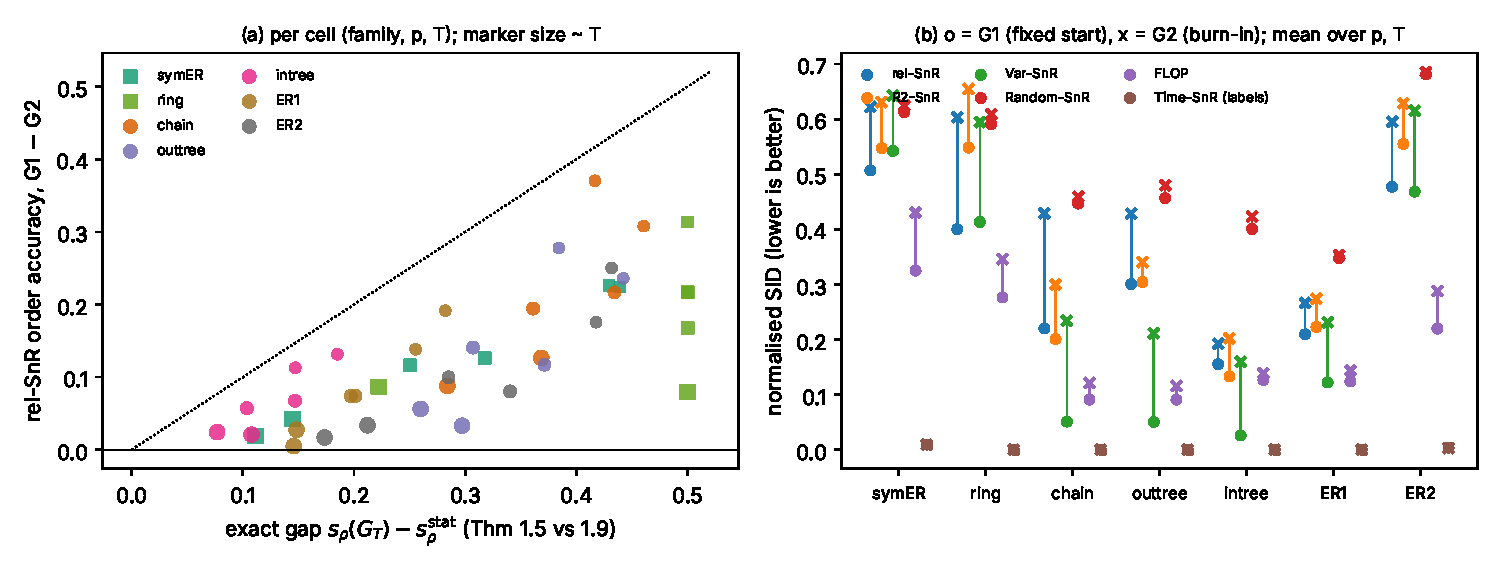
\includegraphics[width=0.48\linewidth]{figs/fig_b1.pdf}\hfill
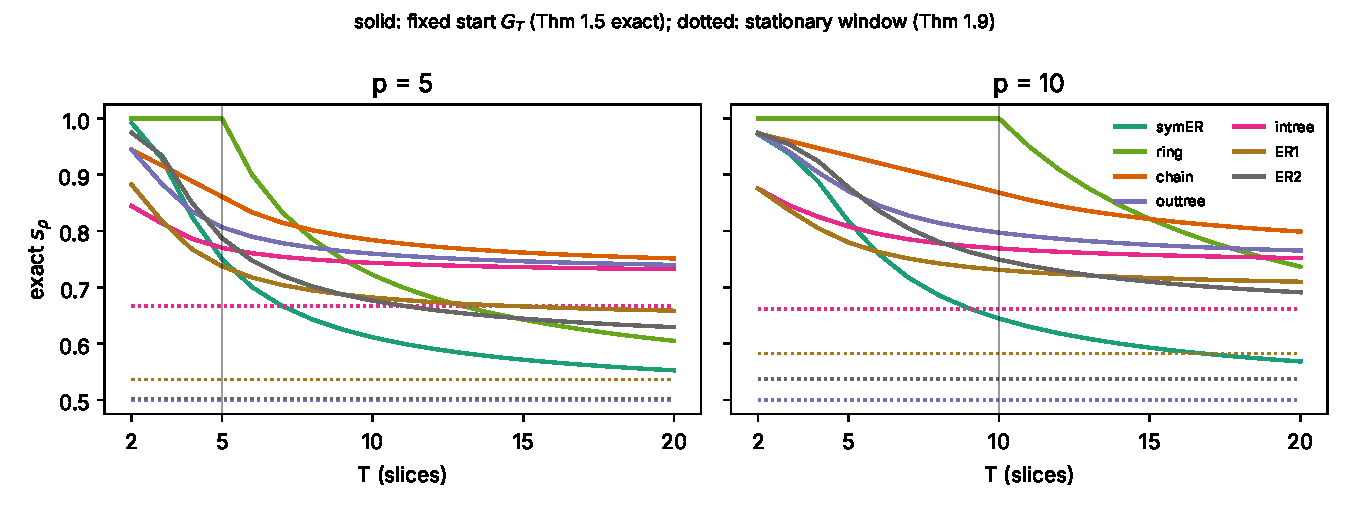
\includegraphics[width=0.48\linewidth]{figs/fig_srho_vs_T.pdf}
\caption{Left: per-cell G1$-$G2 gain in rel-SortnRegress order accuracy
against the exact population gap (all 42 cells below the diagonal and above
0), and normalised SID per method under G1 and G2. Right: exact
$\srho(\GT)$ against $T$, mean over the 30 test graphs per family and $p$.}
\label{fig:srhoT}
\end{figure}

\section{B1-NL: Replication under Nonlinear Dynamics, Signed Weights and Uniform Noise}
\label{app:b1nl}

\textbf{Process.} A separate plan (\texttt{b1nl/PLAN.md}) was committed before
any algorithm score; two notes (a faster but output-identical diagnostic, and
the limited power of sanity rule S1) were added after the validation run and
before the test run. No threshold, hypothesis or seed changed. The test run
(5{,}040 data sets) was run once.

\textbf{Design.} As B1 (\cref{app:b1}) with the B1 code imported unchanged:
seven families, $p\in\{5,10\}$, $T\in\{3,5,10\}$, $n=1000$, G1 against G2
(burn-in 100), R-het and R-std. Three parametrisations. NL: additive VAR with a
linear self-loop and cross terms $w\,g(x)$, $g$ drawn from $\tanh$, $\sin$ and
$(x+x^2/2)/(1+x^2/4)$, positive $w$, stability by scaling the Lipschitz-bound
matrix to spectral radius at most $0.8$. SGN: linear, all weights
$\pm\mathrm{Unif}(0.5,1)$. SGNU: SGN with uniform noise. New seeds (25 graphs per
family and $p$ for NL and SGN, 10 for SGNU); PC and R-eq dropped and G2s
replaced by a 500-step burn-in, to fit one core (stated in the plan).

\textbf{Results.} H1 (same rule as B1) supported in all three: 5/5 families
Holm-significant ($p\le1.4\cdot10^{-9}$); pooled gain $+0.108$ $[0.100,0.116]$
(NL), $+0.137$ $[0.128,0.146]$ (SGN), $+0.137$ $[0.123,0.152]$ (SGNU); positive in
all 126 cells. Tracking: Spearman $0.68$, $0.82$, $0.78$ (slopes $0.34$, $0.56$,
$0.56$). Under NL the correlation-count estimator recovers about $65\%$ of the
graph relatives (recall $0.67$ under G1, $0.62$ under G2), which explains the
smaller slope, as stated before the run. Under signed weights sample relatives
can deviate from graph relatives (out-trees under G2: estimated
rel-sortability $0.455$), yet the gain is as large as in B1. H3: one
Holm-significant SHD swap under NL ($R^2$-SortnRegress against the random order,
chains, $p=10$, $T=10$), none under SGN, not testable for SGNU (10 seeds, stated
in the plan). By the plan's rule H3 is therefore supported under NL, but on a
substantively minor swap, and we do not count it as a replication of B1's
swaps; B1's rel- against $R^2$-SortnRegress chain swap was not detected on SHD
at this replication's power, although the interaction replicates
(\cref{app:b1x}). Without PC, 5 of B1's 11 swap types cannot occur. FLOP is the
best label-free method run there under both generators in every configuration. The
var/rel split holds: Var-SortnRegress gains $+0.19$, $+0.24$, $+0.24$ raw and
about $0$ standardised; rel-SortnRegress $+0.11$, $+0.15$, $+0.14$. Sanity rules
pass (S1 at most $0.015$; mixing error at most $5.6\cdot10^{-5}$).

\begin{figure}[h]
\centering
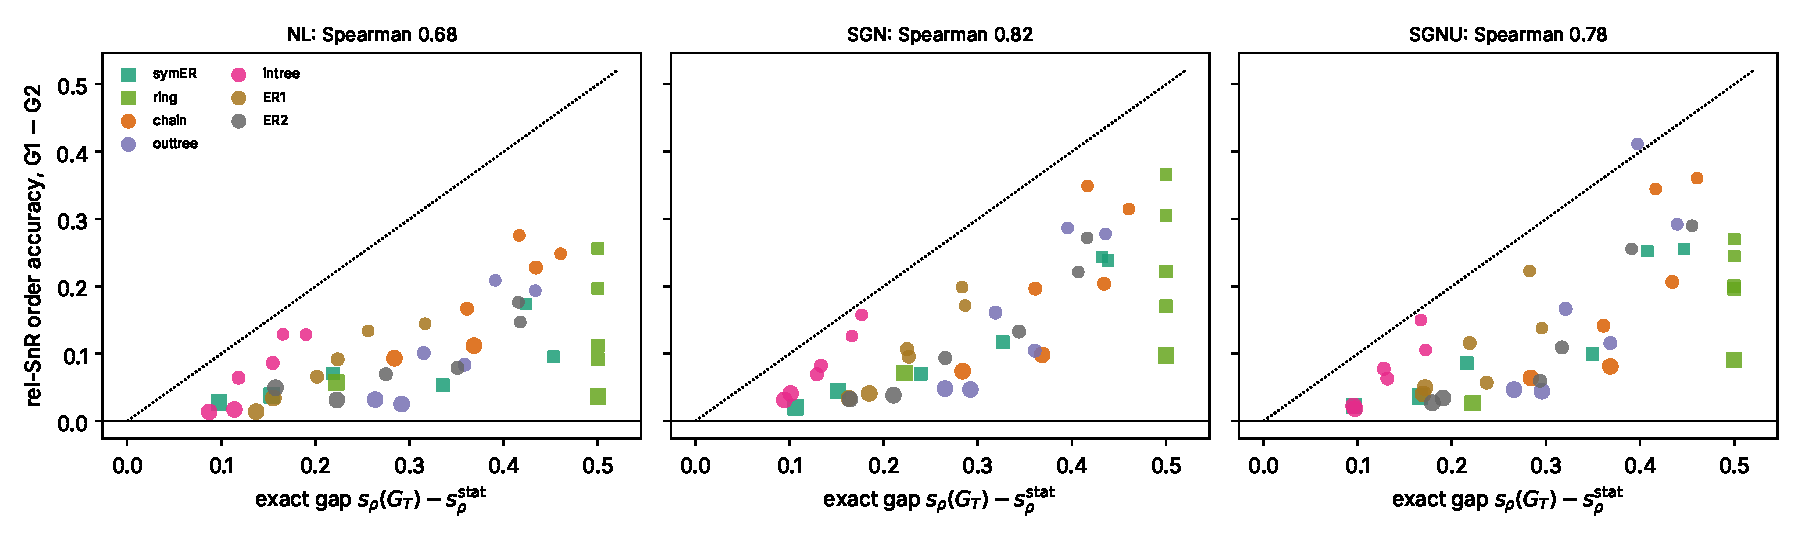
\includegraphics[width=0.7\linewidth]{figs/fig_b1nl.pdf}
\caption{B1-NL: per-cell G1$-$G2 gain in rel-SortnRegress order accuracy
against the exact population gap, for NL, SGN and SGNU.}
\label{fig:b1nl}
\end{figure}

\section{Competitive Learners, Re-Analysis, Detectability Oracle and Generator Survey}
\label{app:b1x}

Material in \texttt{b1x/} and \texttt{lit3/} of the supplement. The learner
extension is a planned experiment; the re-analysis and the oracle are post hoc
and use no new data.

\textbf{Learner extension: process and design.} The plan (\texttt{b1x/PLAN.md}),
code and a validation timing were committed and pushed before any score
(\cref{app:prereg}); the test run took 4.21\,h on one core and was analysed
once, with no deviation (the size rule kept 12 seeds after a projected 4.35\,h).
B1's generators and SEM, new seeds: families ring, chain, in-tree and
ER($c{=}2$), $p\in\{5,10\}$, $T\in\{3,5\}$, 12 graphs per (family, $p$), i.e.\ 96
summary graphs and 384 data sets (G1 and G2), each analysed raw and
standardised with time labels hidden. DAGMA linear (\texttt{dagma} 1.1.1,
$\lambda=0.03$), NOTEARS linear (the authors' reference code, $\lambda=0.1$),
GOLEM-EV/NV (a numpy port of the authors' code with the same score, optimiser,
defaults and post-processing, gradient-checked; $p=5$ only, as planned), all
thresholded at $0.3$; FLOP, the SortnRegress baselines and the empty graph as
comparators; PCMCI+ (tigramite, ParCorr, $\tau_{\max}=1$) on the time-indexed
data as a labels-using reference. Metrics: SHD$/|E|$ (empty graph $=1$),
normalised SID, ancestral order accuracy; unit of inference the summary graph.
T$=10$ and the families symER, out-tree and ER($c{=}1$) were excluded for run time.

\textbf{Verdicts.} HX1 (some raw continuous method Holm-significantly favoured
by the fixed start): supported; all four raw variants improve on all three
metrics (DAGMA SHD$/|E|$ $-0.548$ $[-0.663,-0.438]$, SID $-0.147$, order
accuracy $+0.197$; NOTEARS $-0.419$, $-0.127$, $+0.156$; GOLEM-EV $-0.491$,
$-0.182$, $+0.225$; GOLEM-NV $-0.409$, $-0.193$, $+0.232$; Holm $\le4\cdot10^{-8}$).
HX2 (opposite-sign, both Holm-significant rank change against FLOP on
SHD$/|E|$, 64 tests): supported, two changes, both on in-trees: DAGMA$-$FLOP
$-0.218$ under G1 (Holm $0.012$) and $+0.306$ under G2 ($1.4\cdot10^{-5}$);
NOTEARS$-$FLOP $-0.176$ ($0.0011$) and $+0.193$ ($0.020$); the same two appear on
SID and order accuracy, and DAGMA's persists without first-slice pairs ($0.08$ /
$0.73$ against FLOP's $0.30$ / $0.37$). HX3 (standardisation removes the gain):
DAGMA's SHD gain removed ($-0.005$ $[-0.027,0.016]$), all other pairs reduced
but not removed by the plan's rule; on order accuracy the standardised effect is
significantly negative for DAGMA ($-0.064$), GOLEM-EV ($-0.093$) and GOLEM-NV
($-0.097$), and NOTEARS keeps $+0.036$. rel-SortnRegress replicates ($+0.187$
$[0.169,0.205]$), and B1's chain swap of rel- against $R^2$-SortnRegress recurs
on the new seeds. No fit failed; NOTEARS on standardised data returned a cyclic
graph in $15.6\%$ of data sets (SID missing for 60 of 384). Best label-free
method by mean SHD$/|E|$ per (family, $p$): FLOP in 8/8 cells under G2; under G1
DAGMA on chains with $p=5$ ($0.09$ vs $0.10$) and on in-trees with $p=10$ ($0.06$ vs
$0.33$), NOTEARS on in-trees with $p=5$ ($0.09$ vs $0.27$). Raw continuous methods
beat the empty graph on average under both generators but are worse than it
on chains under G2 ($1.14$--$1.25$). Standardised DAGMA and GOLEM orient most
tree edges backwards under G1 (order accuracy $0.26$--$0.27$). The gains and
the reversals are largest on chains and in-trees, where G1 makes the window
almost perfectly var-sortable (Var-SortnRegress $0.95$--$0.96$), and absent or
reversed on rings and ER($c{=}2$). This is consistent with a var-sortability
effect, but the experiment does not establish it.

\textbf{Predictions of the plan and what the attribution rests on.} The plan
stated three predictions. For HX1 it predicted favourable effects on raw data
for all continuous methods; this held. For HX2 it predicted no rank change
against FLOP on SHD$/|E|$; this failed (two changes). For HX3 it predicted
``reduced, not removed'' for DAGMA and NOTEARS on order accuracy, because some
scale-free gain should survive standardisation. By the plan's rule both were
labelled ``reduced, not removed'', but for DAGMA the standardised effect is
negative ($-0.064$), so no gain survives; for NOTEARS a gain survives
($+0.036$ order accuracy, $-0.077$ SHD$/|E|$, $-0.073$ SID, all
Holm-significant). The standardised runs are a weak test of the attribution
to var-sortability. Standardised DAGMA and GOLEM have order accuracy below
$1/2$ under both generators (DAGMA $0.35$ / $0.41$, GOLEM $0.31$--$0.33$ /
$0.41$--$0.42$), so they cannot show a scale-free effect of either sign.
NOTEARS's remaining gain is a scale-free start effect on a competitive
method. The fixed start also raises $R^2$-sortability, which is scale free
and outside our theory, and we did not separate it. In B1 the gain in
Var-SortnRegress order accuracy is the same on rings ($+0.224$) and chains
($+0.231$), while the learners gain on chains and not on rings; the
explanation by levels ($0.73$ against $0.93$ under G1) was made after the
results. A control that rescales each data set to the other generator's
marginal variances would test the attribution; it has not been run. GOLEM
did not overtake FLOP on in-trees (G1 differences $-0.011$ and $-0.042$, Holm
$1$ and $0.46$). \Cref{tab:b1x} omits GOLEM-EV (SHD$/|E|$ $0.44$ / $0.93$ raw)
and standardised GOLEM ($0.97$ / $1.30$ EV, $0.95$ / $0.99$ NV).

\textbf{Re-analysis of B1 and B1-NL (post hoc).} Graph-cluster bootstrap CIs
(10{,}000 resamples, the three horizons of a graph kept together) are narrower
than data-set bootstrap CIs, because $T$ is a fixed design
factor; they are used in \cref{tab:b1}. Tracking: cell-level Spearman $0.80$
$[0.76,0.82]$, unit-level $0.62$ $[0.59,0.64]$, slope $0.53$ $[0.50,0.56]$ in B1;
$0.68$/$0.44$/$0.34$ (NL), $0.82$/$0.64$/$0.56$ (SGN), $0.78$/$0.62$/$0.56$ (SGNU);
graph-cluster permutation $p\le10^{-4}$ in all four (the floor). Interactions
$I=[m_1-m_2](\mathrm{G1})-[m_1-m_2](\mathrm{G2})$ per graph: Holm-significant in
294/595 (B1), 113/420 (NL), 232/420 (SGN) pair$\times$cell SHD tests and 0 for
SGNU (10 graphs cannot pass Holm). In-tree Var-SortnRegress$-$FLOP on SHD:
$-68.4$ $[-77.0,-60.4]$ (B1), $-49.9$ (NL), $-75.5$ (SGN), $-75.5$ (SGNU); SID
$-0.12$ in all four. Chain rel-$-R^2$-SortnRegress: SID and orientation
interactions replicate at $60$--$80\%$ of B1's size; the family-pooled SHD
interaction is about $0$ in B1-NL, but in B1's swap cell ($p=10$, $T=3$) it keeps
its sign ($-52$, $-16$, $-32$). Empty-graph reference (B1, all families, G1 / G2,
SHD$/|E|$): rel- $1.05$/$1.70$, $R^2$- $1.33$/$1.96$, Var- $0.61$/$1.39$,
random $1.72$/$2.04$, FLOP $0.27$/$0.46$, PC $0.40$/$0.64$; the empty graph has
normalised SID $0.50$. Order accuracy without edges leaving the first window
slice (non-SC families): rel-SortnRegress $+0.089$ $[0.079,0.100]$ (B1), $+0.067$
(NL), $+0.087$ (SGN), $+0.095$ (SGNU). Multiplicity: each claim of
B1, B1-NL, B3 and the extension gets one claim-level $p$ (the $k$-th smallest
Holm $p$ for ``$k$ of $m$ families'' rules, the best swap for swap rules, the
cluster permutation for tracking, the plan's Holm $p$ for B3); Holm over the 21
claims at family-wise $0.05$ keeps all but B1-NL H3-SGN ($p=0.108$); the closest
survivors are B1 H3 (Holm $0.0079$), B1-NL H3-NL and HX2 (both $0.033$). Several
claim $p$ are at resolution floors ($10^{-4}$ for permutations, $10^{-5}$ for
B3's sign flips).

\textbf{Detectability calculation (``oracle''; post hoc).} For every B1 test graph, parameter set
and horizon we propagated the exact window covariance (G1:
$\Sigma_{t+1}=A^\top\Sigma_tA+D$ from $\Sigma_1=D$; G2: after the same 100
burn-in steps). Population relatives ($|\rho|>10^{-20}$) reproduce the exact
$\srho$ of \cref{thm:limit,thm:stat} in all 2{,}520 cases. The oracle replaces
each sample correlation in rel-SortnRegress's count by the probability that
the Fisher-$z$ statistic at $n=1000$ exceeds the algorithm's threshold
($\varepsilon=0.062$) and predicts each edge's order accuracy as
$P(c_i<c_j)+\tfrac12P(c_i=c_j)$, treating the indicators as independent. It uses
no simulated data. Against the observed G1$-$G2 gain: cell level Spearman
$0.99$, $R^2=0.97$, slope $1.03$, intercept $-0.010$; unit level $R^2=0.61$
against $0.34$ for the exact gap (difference $+0.27$ $[0.23,0.30]$); in a joint
regression the gap's coefficient is $-0.063$ over cells and $-0.039$ over graph--horizon units. Predicted G1 / G2 levels: chain
$0.756$/$0.528$ (observed $0.749$/$0.532$), ring $0.702$/$0.503$ ($0.687$/$0.507$),
in-tree $0.746$/$0.677$ ($0.743$/$0.673$). Without slice-1 edges the non-SC gain
is predicted to fall from $+0.130$ to $+0.096$ (observed $+0.125$ to $+0.089$).
What this shows and does not show: the calculation is the expectation of
rel-SortnRegress under the exact covariances of each generator, so the
agreement says that the simulated gain has the size those covariances imply
and that the independence approximation is adequate. It uses the full
start-dependent covariances, so it includes every way in which the start
changes pairwise correlations: pairs that are relatives under the fixed start
only (the mechanism of \cref{sec:exact}) and pairs that are relatives under
both starts but differ in correlation strength (a transient that needs no
graph argument). We did not decompose the predicted gain into these two
parts, so the calculation does not show that the gain is due to the first.
The exact gap therefore gives a ranking and a rough scale; all 42 cells have the same sign, so the sign tests nothing.

\textbf{Generator survey.} We read the source code of tigramite 5.2.10.1
(\texttt{structural\_causal\_process}: zeros plus noise, burn-in
$\lfloor0.2T\rfloor$; \texttt{var\_process}: i.i.d.\ $N(0,1)$ start, no burn-in),
the CDML generator \citep{lawrence2021dgp} (zeros, $2\tau_{\max}$ steps dropped),
CausalTime \citep{cheng2024causaltime} (rollouts of 20 steps from a real-data
window, no burn-in, in the demo), UUMCdata \citep{herman2025unitless} (exact
stationary start), causalnex 0.12.1 (zeros, burn-in 100 or more; data with lag
labels), the Neural-GC VAR and Lorenz-96 simulators \citep{tank2021neural}
(burn-in 100 and 1000) and gCastle 1.0.4 (no continuous time-series
simulator; its Hawkes simulator starts with an empty history). cdt, causaldag,
causal-learn and lingam ship no time-series benchmark generator.
\citet{lohse2025sortability} state a burn-in without its length. The
time-unrolled construction of \citet{reisach2026topological} starts at $t=1$
and gives every slice to an i.i.d.\ method as a separate variable; its code is
not public, so only the graph-level start is verified. CauseMe's documentation
could not be opened with TLS verification, so we make no claim about it. File
and line references are in \texttt{lit3/GENERATOR\_SURVEY.md}. Reading of
exposure: the burn-in lengths above can be compared with
$\Delta\tau_{\max}$, which concerns the graph artefact only. The variance
artefact needs the start to be far from the stationary distribution relative
to the mixing time of the process, which depends on the spectral radius of
the generated coefficients; we computed no mixing time for any of these
generators, so we do not grade them on it. All of them except the
time-unrolled construction produce a single record with time order for
time-series methods, so neither artefact applies to them as shipped; they
would be exposed only if windows from their first steps were given to a
method that ignores time order.

\section{B3: Discriminating Test of the Source-SCC Rule on Held-Out Data}
\label{app:b3}

\textbf{Process.} The plan (\texttt{b3/PLAN.md}, with an OSF-formatted copy) was
pushed before any byte of the held-out data was read; zip CRC-32 values were
taken from the remote archive directory before the plan and SHA-256 hashes at
download. The plan is internally time-stamped only: it was not posted to an
external registry before data access, and results were committed 3--4 minutes
after the plan. A disclosed development check on study-3 data from the same
device had shown every colour edge to be detectable, so the primary outcome
was expected.

\textbf{Data.} Causal Chambers experiments not previously downloaded by the
project. H1 (primary): \texttt{lt\_camera\_walks\_v1}, experiments
\texttt{ar\_1\_uniform\_\{ref, pol\_1\_90, pol\_12\_30\}}: five independent
stationary AR(1) actuators drive the light sensors, so the colour block is
one weak component with three source SCCs; $3\times30{,}000$ steps, 30 units of
3{,}000. H2 (co-primary): \texttt{lt\_camera\_v1/scm\_5\_red} and
\texttt{scm\_5\_blue}, i.i.d.\ data from the collider R$\to$G$\leftarrow$B, 20
units. Secondary: \texttt{scm\_5\_green}, \texttt{scm\_4\_green},
\texttt{scm\_4\_blue}, and \texttt{scm\_4\_red} as a single-source control.

\textbf{Test.} E1's estimator unchanged. Competitors: constant $1/2$, the
weak-component-size rule, the theorem on the design graph $G_D$, and E1's
eight naive rules. Primary set $D^*$: instances where the theorem and the
weak-component rule disagree ($56\%$ of instances for H1, $47\%$ for H2, from
graph-only computation before the plan); on $D^*$ the prediction is the same
on $G_{\mathrm{lin}}$ and $G_D$. Failure of the estimator pushes observed values
towards the tie rules, so a pass on $D^*$ cannot come from ties. Sign-flip
tests over units, Holm, family $\alpha=0.025$; pass requires $\Delta\le-0.10$
against every competitor that disagrees on $D^*$.

\textbf{Results.} H1: on 2{,}361 instances, counts sorted as predicted in
2{,}356; $\Delta=-0.498$ against both tie rules, 30/30 units, $p\approx10^{-5}$;
non-relatives declared dependent $0.054$, relatives detected $0.990$. H2:
$\Delta=-0.50$ against the tie rules and the sensor indicator, 20/20 units;
R$\to$G sorted 264/264 when B is observed and tied 123/123 when not. S1
(predicted tie, detected edge; 1{,}251 instances): theorem beats the eight
naive rules ($\Delta=-0.43$, 30/30 units) and the theorem on $G_D$ narrowly
($\Delta=-0.21$, 21/30 units, Holm $p=0.021$). No stop condition met.

\textbf{Failures.} \texttt{scm\_4\_blue}: the tie rule is significantly better
($\Delta=+0.115$, 0/10 units, reverse $p=0.001$); post hoc, the intervened blue
channel ranges over 1--13 of 255 levels, so none of its edges is detected, and
the pooled detection prerequisite ($0.837$) did not catch this. The pooled
secondary analysis still passes, in 20/30 units. In
\texttt{ar\_1\_uniform\_pol\_1\_90} the polariser linear-zero refinement of
\cref{app:e1} fails (polarisers correlate with ir$_3$, vis$_3$ at
$|r|\approx0.2$--$0.28$; $G_D$ matches $0.959$ against $0.041$ for
$G_{\mathrm{lin}}$); H1 does not depend on it. Deviations: the inputs of two
experiments do not reproduce from the published generator seeds (ranges
match; not gating).


%=============================================================================
\section{Proofs for Sections~\ref{sec:labels} and~\ref{sec:ident}}
\label{app:ident}

\Cref{prop:nogain} is proved in the main text. The proofs below are paper
proofs; none is machine-checked. Notation as in \cref{sec:ident}.

\begin{proof}[Proof of \cref{prop:slices}]
(a) Every edge of $\GT$ goes from a slice $t$ to slice $t+1$, so a directed
path ending in $v(t)$ has at most $t-1$ edges, and the self-chain
$v(1)\to\dots\to v(t)$ has exactly $t-1$. Graph isomorphisms preserve height,
so two labellings of the same column DAG as unrollings with self-loops put the
same columns in slice $t$, and $T$ is the largest height and $p$ the number of
columns of height one.
(b) The column DAG of the ring $i\to i+1$ with self-loops has the edges
$(i,t)\to(i,t{+}1)$ and $(i,t)\to(i{+}1,t{+}1)$. With the new unit label
$i'=i-t \pmod p$ the first family reads $i'\to i'-1$ and the second
$i'\to i'$, which is the unrolling of the reversed ring with self-loops.
(c) Without loops the unrolling of $0\to1$ has the edges $0(t)\to1(t{+}1)$,
$t<T$, which are pairwise disjoint; every one of them has a tail of height one
and a head of height two.
\end{proof}

\begin{proof}[Proof of \cref{prop:mec}]
Two parents $i(t)$ and $k(t)$ of a node $j(t{+}1)$ lie in the same slice and
are not adjacent, so every node with at least two parents is an unshielded
collider, and all its incoming edges have the same direction in every member
of the class. The remaining edges are those into nodes with exactly one
parent; since every node $j(t{+}1)$ has the parent $j(t)$, these are the
self-chain edges of loop-only units. Fix such a unit $j$ and a member of the
class. On the chain $j(1),\dots,j(T)$ the member has no collider (a collider
at a chain node would be unshielded, as chain neighbours at distance two are
not adjacent, and $\GT$ has none there), so the chain is oriented away from
one of its nodes $j(s)$. Conversely, re-rooting the chain at any $j(s)$ keeps
the skeleton, creates no collider (every chain node still has at most one
parent, because a loop-only unit has no parent outside its chain), removes
none, and creates no cycle (a directed cycle would have to enter the chain
from outside, and no edge does). The chains of different loop-only units are
disjoint and can be re-rooted independently, which gives $T^{m_0}$ members.
\end{proof}

\begin{proof}[Proof of \cref{prop:fixident}]
(a) Let $G'$ be the column DAG of a sparsest representation. $\Sigma$ is
Markov to $G'$, because the representation is a linear structural equation
model on $G'$ with independent noise terms (the start covariance is diagonal
under the fixed-start law). $G'$ has $(T-1)|\mathrm{supp}\,A'|$ edges, at most
as many as $\GT$, because the true parameter is itself a representation. As
the distribution is faithful to $\GT$, a DAG to which it is Markov has at
least as many edges as $\GT$, with equality only if it is Markov equivalent
to $\GT$ \citep[Theorem~4]{chickering2002optimal}. By \cref{prop:mec}, $G'$ is
$\GT$ with the chains of some loop-only units re-rooted. $G'$ is also an
unrolling with self-loops, so by \cref{prop:slices}(a) every edge of $G'$
joins consecutive heights, and every node of height at least two has a
self-parent, with different nodes having different self-parents. Re-root the
chain of a loop-only unit $j$ at $j(s)$. If $1<s<T$, then $j(s)$ has no parent
in $G'$, and $j(s{-}1)$ and $j(s{+}1)$ both have $j(s)$ as their only parent,
so both would have the self-parent $j(s)$: impossible. If $s=T$, then $j(1)$
has height $T$ in $G'$; if $j$ has a child $k\ne j$ in $\GS$, the edge
$j(1)\to k(2)$ is an edge of $G'$ (it enters a node with two parents or more,
namely $j(1)$ and $k(1)$), which gives $k(2)$ the height $T+1$: impossible. So
only isolated units can be reversed, and only as a whole.
(b) Let $v_t$ be the variance of $x_j(t)$, $v_{t+1}=a^2v_t+d$. The reversed
chain is a representation iff the regression of $x_j(t)$ on $x_j(t{+}1)$ has
the same coefficient $a v_t/v_{t+1}$ and the same residual variance
$d\,v_t/v_{t+1}$ for all $t\in\{1,\dots,T-1\}$, i.e.\ iff $v_t/v_{t+1}=r$ does
not depend on $t$. For $T=2$ there is one transition and nothing to compare.
For $T\ge3$, $v_3-v_2=a^2(v_2-v_1)$ gives
$\tfrac1r(\tfrac1r-1)=a^2(\tfrac1r-1)$, so $r=1$, which is stationarity, or
$1/r=a^2$, which forces $d=0$ and is excluded. If $r=1$ for the first two
transitions then $v_t$ is constant for all $t$.
(c) follows from (a) and (b).
\end{proof}

\begin{proof}[Proof of \cref{prop:nonident}]
(a) In the truth, $a_2=\alpha a_1+\varepsilon_a$ and
$b_2=\beta a_1+\gamma b_1+\varepsilon_b$, with an arbitrary covariance of
$(a_1,b_1)$. Take the units $a'=(a_1,a_2)$ and $b'=(b_2,b_1)$, i.e.\ the first
slice $\{a_1,b_2\}$ and the second slice $\{a_2,b_1\}$. Then
$a_2=\alpha a_1+0\cdot b_2+\varepsilon_a$ and $b_1=\beta'a_1+\gamma'b_2+\eta$,
where $\eta$ is the residual of the linear regression of $b_1$ on
$(a_1,b_2)$. By construction $\eta$ is uncorrelated with the new first slice;
it is a linear function of $(a_1,b_1,\varepsilon_b)$ and therefore
uncorrelated with $\varepsilon_a$, and $\varepsilon_a$ is uncorrelated with
$(a_1,b_2)$. So the new innovation covariance is diagonal and uncorrelated
with the new first slice, whose covariance is free. The new self-loop
coefficients are $\alpha\ne0$ and $\gamma'$, which is non-zero whenever
$\gamma\ne0$ (the partial correlation of $b_1$ and $b_2$ given $a_1$ is
non-zero); the support of the new transition matrix has three entries when
$\beta'\ne0$ and two otherwise, so the new representation has no more edges
than the truth.
(b) A stationary Gaussian AR(1) process has a symmetric autocovariance, so
the reversed window has the same covariance, and an isolated unit is
uncorrelated with all other columns.
(c) $\Gamma=\sigma^2(I-A^2)^{-1}$ solves $\Gamma=A\Gamma A^\top+\sigma^2I$ and
commutes with $A$. The time-reversed stationary process has transition matrix
$\Gamma A^\top\Gamma^{-1}=A$ and innovation covariance
$\Gamma-A\Gamma A^\top=\sigma^2I$, so the reversed window is a representation
with the same support.
\end{proof}

\textbf{On \cref{conj:window}.} Let $H$ be $\GT$ plus a complete DAG on the
first slice. Under the stated faithfulness, the argument of
\cref{prop:fixident}(a) shows that the DAG of a sparsest representation (its
unrolling plus a complete DAG on its first slice) is Markov equivalent to $H$,
hence has the same skeleton $U$. In $H$ the edges between slices 1 and 2 are
not fixed by colliders, because the parents of a slice-2 node lie in the
first-slice clique. If the only partition of the nodes of $U$ into $T$ layers
of size $p$, with edges inside layer 1 or between consecutive layers and a
perfect matching between consecutive layers, is the true one, the conjecture
follows; the reversed layering is excluded when slice $T$ is an independent
set of $U$ and slice 1 is not. We checked uniqueness by hand for the summary
edge $a\to b$ with self-loops and $T=3$; \cref{prop:nonident}(a) shows that it
fails for $T=2$. We have no proof for general graphs, and the case in which
the first slice is not a clique in $U$ is not covered.

\end{appendices}

\bibliography{refs}

\end{document}
